% Magic comments - Informa ao compilador algumas regras de execução, como tipo de compilação ou codificação do texto
% !TeX root = monografia-online-petri-net-simulator.tex
% !TeX encoding = UTF-8
% !BIB TS-program = XeLaTex
% !backend = biber

%% abtex2-modelo-trabalho-academico.tex, v-1.9.2 laurocesar
%% Copyright 2012-2014 by abnTeX2 group at http://abntex2.googlecode.com/
%%
%% This work may be distributed and/or modified under the
%% conditions of the LaTeX Project Public License, either version 1.3 of this license or (at your option) any later version.
%%
%% This work has the LPPL maintenance status `maintained'.
%%
%% INÍCIO DAS CUSTOMIZAÇÕES PARA A UNIVERSIDADE FEDERAL DE OURO PRETO%%

%% 2022.3.30 13h15 Danny Tonidandel
%% Altera as definições de capa, alterando  o comando, inserindo figuras próprias da Universidade e alterando a disposição dos elementos na contra-capa
%% Remove itens de abstract em francês
%% Altera disposição dos elementos na folha de aprovação
%% Altera o conteudo dos capítulos para um arquivo único.
%% Personalização do estilo biblatex-abnt para adequação à normaABNT 6023:2018
% Reseta contadores das notas de rodapé em cada capítulo
% Insere comandos para exibir uma caixa colorida de fundo cinza para notas explicativas, à escolha do autor

%% 2017.5.31 21h13 Danny Tonidandel
%% Altera nome de arquivo de logomarca
%% remove resumos em espanhol e italiano
%% Insere exemplos para elaboração de tabelas
%% Insere tabela de cronograma de atividades (para projeto de pesquisa)

%% FIM DAS CUSTOMIZAÇÕES PARA A UNIVERSIDADE FEDERAL DE OURO PRETO

%% This work consists of the files
% monografia-online-petri-net-simulator.tex
% referencias.bib
%%
% --------------------------------------------
% ----------------------------------------------
% abnTeX2: Modelo de trabalho Academico (tese de doutorado, dissertacao de

% mestrado e trabalhos monograficos em geral) em conformidade com
% ABNT NBR 14724:2011: Informacao e documentacao - Trabalhos academicos -
% Apresentacao
% ------------------------------------------------------------------------
% ------------------------------------------------------------------------

\documentclass[
	% -- opções da classe memoir --
	12pt,				% tamanho da fonte
	openright,			% capítulos começam em pág ímpar (insere página vazia caso preciso)
	oneside,			% p/ impressão verso e anverso: twoside
	a4paper,			% tamanho do papel.
	% -- opções da classe abntex2 --
	%chapter=TITLE,		% títulos de capítulos convertidos em letras maiúsculas
	%section=TITLE,		% títulos de seções convertidos em letras maiúsculas
	%subsection=TITLE,	% títulos de subseções convertidos em letras maiúsculas
	%subsubsection=TITLE,% títulos de subsubseções convertidos em letras maiúsculas
	% -- opções do pacote babel --
	english,			% idioma adicional para hifenização
	brazil				% o último idioma é o principal do documento
	]{abntex2}

% ---
% Pacotes básicos
% ---

\usepackage{graphicx} 	% gráficos
\usepackage[table,xcdraw]{xcolor}	% tabelas
\graphicspath{{figuras/}} % pasta para figuras
\DeclareGraphicsExtensions{.pdf,.eps,.svg,.png,.jpg,.bmp}

\usepackage{indentfirst} % para identação no primeiro parágrafo
\usepackage{booktabs}
\usepackage{microtype} 	% justificação
\usepackage{verbatim}
\usepackage{placeins}
\usepackage{listings} % pacote para inserção de código

\lstdefinelanguage{JavaScript}{
    keywords={break, case, catch, continue, debugger, default, delete, do, else, finally, for, function, if, in, instanceof, new, return, switch, this, throw, try, typeof, var, void, while, with, let, const},
    sensitive=true,
    comment=[l]{//},
    morecomment=[s]{/*}{*/},
    morestring=[b]',
    morestring=[b]"
}

\lstset{
    language=JavaScript,          % Define a linguagem como JavaScript
   	backgroundcolor=\color{gray!10},
    basicstyle=\ttfamily\footnotesize,         % Fonte básica do código
    keywordstyle=\color{blue},    % Cor das palavras-chave
    commentstyle=\color{gray},    % Cor dos comentários
    stringstyle=\color{red},      % Cor das strings
    breaklines=true,              % Quebra linhas longas automaticamente
    frame=single,                 % Coloca o código em uma caixa
    numbers=left,                 % Adiciona números de linha à esquerda
    numberstyle=\tiny\color{gray} % Estilo dos números de linha
}

\renewcommand{\lstlistingname}{Código} % Altera "Listing" para "Código"



\usepackage{tikz}
\usetikzlibrary{shapes.geometric, arrows}

\tikzset{
	startstop/.style={rectangle, rounded corners, minimum width=3cm, minimum height=1cm, text centered, draw=black, fill=red!30},
	process/.style={rectangle, minimum width=3cm, minimum height=1cm, text centered, draw=black, fill=orange!30},
	arrow/.style={thick,->,>=stealth}
}

\usetikzlibrary{positioning}

% Pacotes de escrita matemática
\usepackage{amsmath,amssymb,unicode-math}


\usepackage{pdfpages} %  anexar pdf diretamente no documento
\usepackage{csquotes}

% Citações


% Opção 2: notas explicativas no sistema autor-data
\usepackage[backend=biber,
% % configuracoes do estilo abnt
 style=abnt,
 sccite, % sobrenomes em caixa alta
 ittitles, % Titulos em italico
 citecount, % contar o número de citações
 scbib, % biliografia em caixa alta
 justify, % alinhamento justificado
 noslsn,
 repeatfields,
 sorting=nty, % ordem alfabetica
 ]{biblatex}

% ARQUIVO COM AS REFERÊNCIAS BIBLIOGRAFICAS
\addbibresource{referencias.bib}

% ---
% Personalização do estilo biblatex-abnt
%Danny A. V. Tonidandel

% Adequa as urls de acordo com normas 6023:2018
\DeclareFieldFormat{url}{\bibstring{urlfrom}\addcolon\addspace \url{#1}}%
\DeclareFieldFormat{urldate}{\bibstring{urlseen}\addcolon\addspace #1}%

% Reseta contadores das notas de rodapé em cada capítulo
\makeatletter
\@addtoreset{footnote}{chapter}
\makeatother

% Pacotes adicionais - podem ser comentados
\usepackage{lipsum}	% para geração de texto aleatório
% ---

%Criação de Teoremas

% buscar documentação no CTAN
\newtheorem{exemplo}{Exemplo}
%\theoremstyle{break}

% ---
% Informações de dados para CAPA e FOLHA DE ROSTO
% ---
\titulo{DESENVOLVIMENTO DE UMA APLICAÇÃO WEB COM O OBJETIVO DE CONSTRUIR E SIMULAR REDES DE PETRI}
\autor{Douglas Meneses Barbosa}
\local{Ouro Preto}
\data{\the\year} % imprime o ano corrente no campo data
\orientador{Prof. Dr. Danny Augusto Vieira Tonidandel}
\coorientador{\color{red}Não definido}
\instituicao{Universidade Federal de Ouro Preto}
\tipotrabalho{Monografia de Graduação}
\preambulo{Trabalho apresentado ao Colegiado do Curso de Engenharia de Controle e Automação da Universidade Federal de Ouro Preto como parte dos requisitos para a obtenção do Grau de Engenheiro de Controle e Automação.}
% ---


% ---
% Aparência do PDF final

% alterando o aspecto da cor azul
\definecolor{blue}{RGB}{41,5,195}

% informações do PDF
\makeatletter
\hypersetup{
     	%pagebackref=true,
		pdftitle={\@title},
		pdfauthor={\@author},
    	pdfsubject={\imprimirpreambulo},
	    pdfcreator={LaTeX with abnTeX2},
		pdfkeywords={ufop}{latex}{decat}{monografia},
		colorlinks=true,   % opções: false, true
    	linkcolor=blue,    % cor de links internos
    	citecolor=blue,    % cor de links na bibliografia
    	filecolor=magenta, % color de links para arquivos
		urlcolor=blue,     % cor de hiperlinks (urls)
}
\makeatother
% ---

% ---
% Espaçamentos entre linhas e parágrafos
% ---

\setlength{\parindent}{1.3cm} % Tamanho do parágrafo


\setlength{\parskip}{0.2cm} % Espaçamento entre parágrafos
% tente também \onelineskip


\makeindex % compila o indice


\begin{document} % Início do documento

\frenchspacing % Retira espaço obsoleto

% Pré-TextualEXTUAIS
% \pretextual

% Capa - obrigatório

\begin{capa}
	\thispagestyle{empty}
		\centering
	\begin{center}
		\begin{minipage}{1\linewidth}
			\centering
			\begin{tabular}{ccc}
				\begin{tabular}{c}
					\\
					
\includegraphics[width=0.9cm]{logo-universidade.jpg}
				\end{tabular}
				&
				\begin{tabular}{c}
					\\
					{\large \imprimirinstituicao} \\
					{\large Escola de Minas} \\
					{\large CECAU - Colegiado do Curso de } \\
					{\large Engenharia de Controle e Automação}
				\end{tabular}
				&
				\begin{tabular}{c}
					\\
					
\includegraphics[width=2.1cm]{logo-unidade-2.jpg}
				\end{tabular}
			\end{tabular}
		\end{minipage}

\centering
\vspace*{1cm}
{\ABNTEXchapterfont\large\imprimirautor}
\vspace*{\fill}

{\ABNTEXchapterfont\bfseries \large \imprimirtitulo}
\vspace*{\fill}

{\large\imprimirtipotrabalho}
\vspace*{\fill}

{\large\imprimirlocal}, {\large \the\year}
%\par
\vspace*{1cm}
	\end{center}
\end{capa}



% Folha de rosto [OBRIGATÓRIO]
\imprimirfolhaderosto
% \imprimirfolhaderosto* se quiser ficha catalográfica

% Ficha bibliográfica [OPCIONAL,segundo determinação CECAU  e DECAT, 29/03/2023]
% \begin{fichacatalografica}
%     \includepdf{fig_ficha_catalografica.pdf}
% \end{fichacatalografica}


% Folha de aprovação - Obrigatório NBR 14724/2011
\begin{folhadeaprovacao}
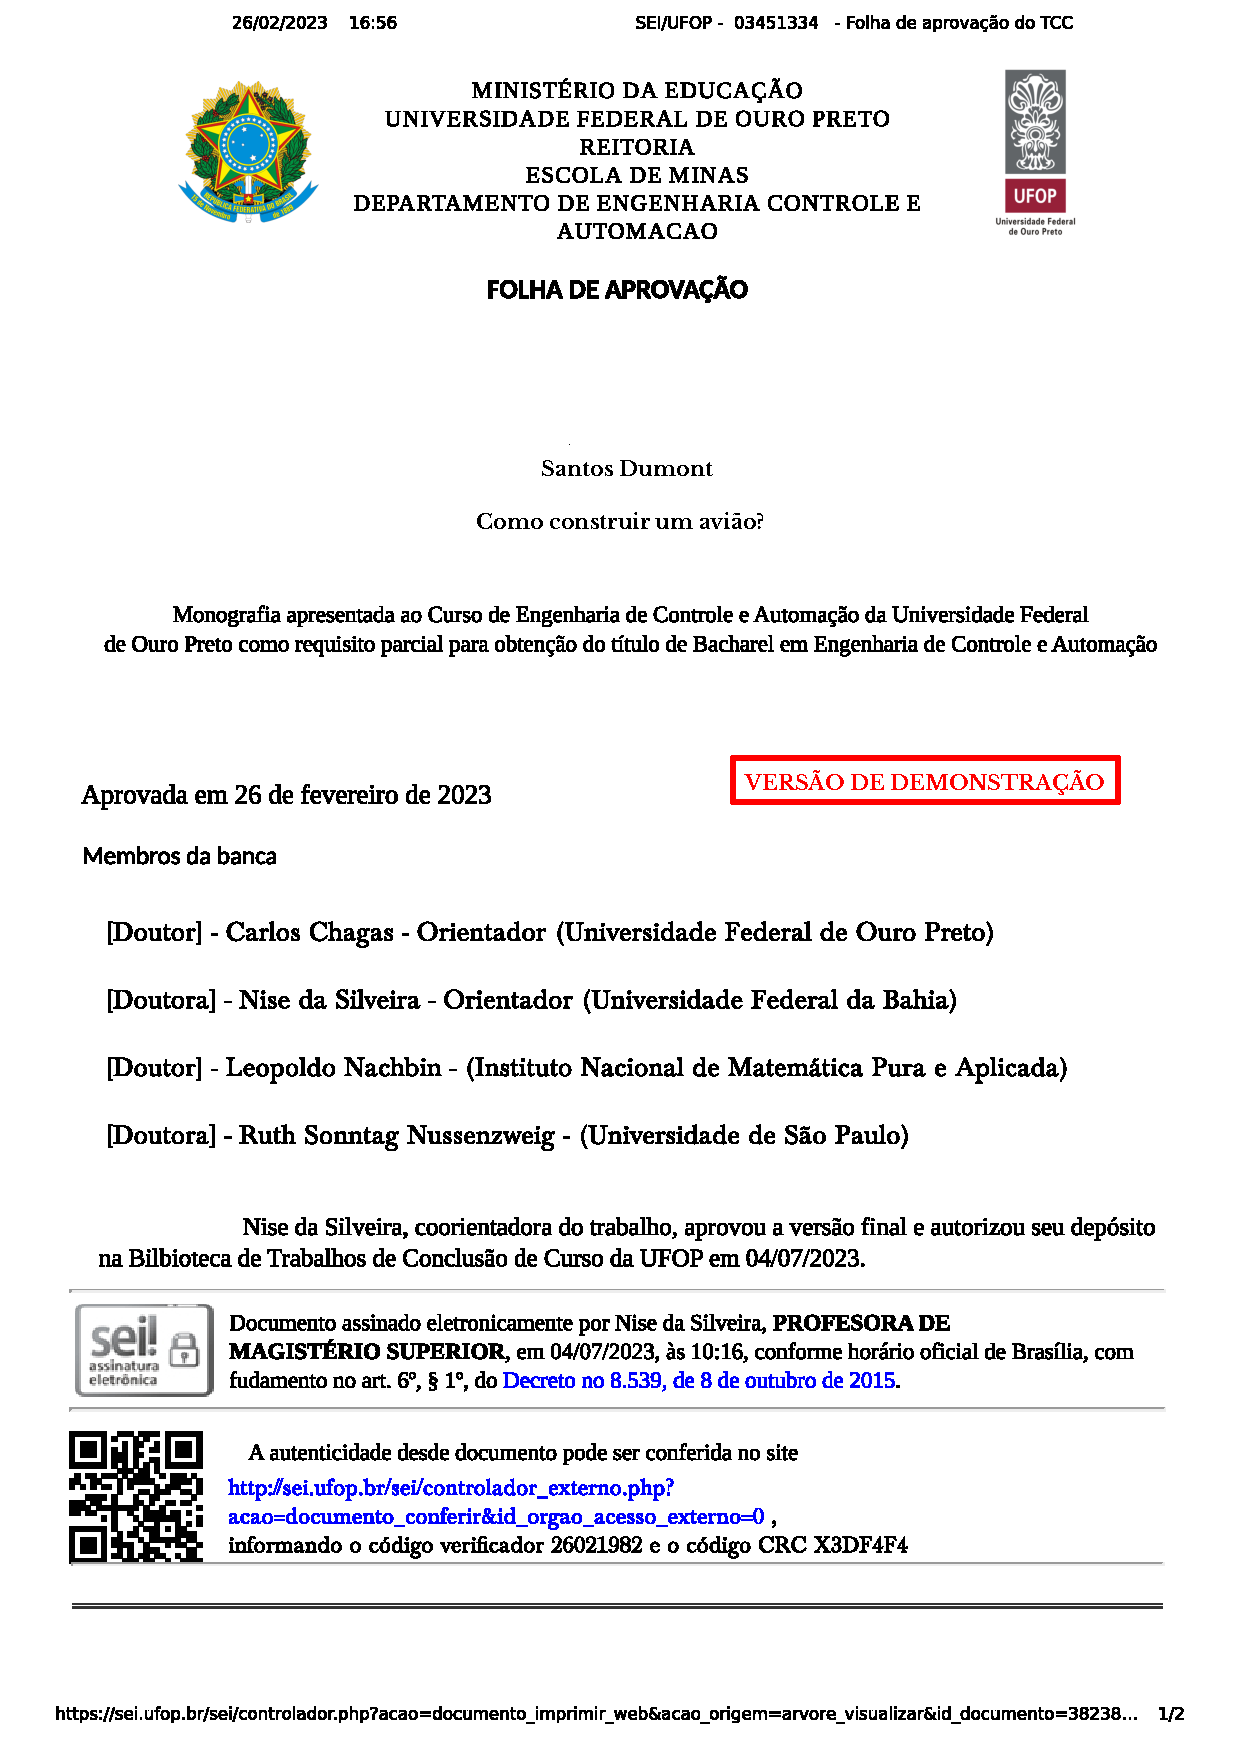
\includepdf{folha-de-aprovacao.pdf}
\end{folhadeaprovacao}


% Agradecimentos - opcional
\begin{agradecimentos}
\noindent Os agradecimentos [são opcionais, e] vem aqui... 
\end{agradecimentos}

% Epígrafe - Opcional
\begin{epigrafe}
    \vspace*{\fill}
\epigraph{\textsl{Júpiter leva 4332 dias para fazer uma revolução.}}{---~Oliver Lodge.}
\end{epigrafe}
% ---

% ---
% RESUMOS
% ---

% resumo em português
\setlength{\absparsep}{18pt} % ajusta o espaçamento dos parágrafos do resumo
\begin{resumo}
 \noindent O resumo deve ressaltar o objetivo, o método, os resultados e as conclusões do documento. A ordem e a extensão
 destes itens dependem do tipo de resumo (informativo ou indicativo) e do tratamento que cada item recebe no documento original. O resumo deve ser precedido da referência do documento, com exceção do resumo inserido no
 próprio documento. (\ldots) As palavras-chave devem figurar logo abaixo do resumo, antecedidas da expressão Palavras-chave:, separadas entre si por
 ponto e finalizadas também por ponto.

 \textbf{Palavras-chaves}: latex. abntex. editoração de texto.
\end{resumo}

% resumo em inglês
\begin{resumo}[Abstract]
 \begin{otherlanguage*}{english}

\noindent This is the english abstract.

   \vspace{\onelineskip}

   \noindent
   \textbf{Key-words}: latex. abntex. text editoration.
 \end{otherlanguage*}
\end{resumo}


% Lista de ilustrações
\pdfbookmark[0]{\listfigurename}{lof}
\listoffigures*
\cleardoublepage
% ---

% % inserir lista de tabelas
% \pdfbookmark[0]{\listtablename}{lot}
% \listoftables*
% \cleardoublepage
% % ---

% % ---
% % Lista de abreviaturas e siglas [OPCIONAL]
% % ---

% \begin{siglas}
%   \item[ABNT] Associação Brasileira de Normas Técnicas
%   \item[abnTeX] ABsurdas Normas para TeX
% \end{siglas}
% % ---

%---
% Lista de símbolos [OPCIONAL]
%---
% \begin{simbolos}
%   \item[$ \Gamma $] Letra grega Gama
%   \item[$ \Lambda $] Lambda
%   \item[$ \zeta $] Letra grega minúscula zeta
%   \item[$ \in $] Pertence
% \end{simbolos}
% ---

% ---
% Sumário
% ---
\pdfbookmark[0]{\contentsname}{toc}
\tableofcontents*
\cleardoublepage


% Reinicia contadores das notas de rodapé
\makeatletter
\@addtoreset{footnote}{chapter}
\makeatother



% ELEMENTOS TEXTUAIS

\textual

% Modelo de capitulo com a introducao, objetivos e estrutura do texto

% --
\chapter[Introdução]{Introdução}

nome da aplicação: Online Petri Net Simulator

Em 1962, Carl Adam Petri, por meio de sua dissertação, mostrou para o mundo a sua criação, as redes de Petri \cite{petri1962kommunikation}. Podemos definir uma rede de Petri como sendo uma ferramenta matemática para modelagem de sistemas concorrentes. Além da modelagem matemática, as redes de Petri podem ser ilustradas graficamente por meio de seus elementos, os lugares, as transições e os arcos. Além disso, com a evolução da industria e da tecnologia, as redes de Petri ganharam ainda mais relevância, uma vez que elas permitem a modelagem de diversos tipos de sistemas, em diferentes áreas. 

A evolução da industria e da tecnologia também culminou com a popularização da internet \cite{lins2013evoluccao}. O surgimento do World Wide Web, em 1990, por Tim Berners-Lee, permitiu aos primeiros usuários da internet, como conhecemos hoje, a interação com um sistema de hipertexto. Com o passar dos anos, as aplicações web se tornaram cada vez mais comuns e sofisticadas. O que antes começou com páginas estáticas evoluiu para aplicações dinâmicas, interativas e de fácil acesso para a maioria das pessoas. Atualmente, se consegue ter uma experiência muito próxima as funcionalidades de um computador pessoal, com aplicações desktop, apenas manipulando abas em um navegador.

Diante da facilidade de acesso a aplicativos web por meio dos navegadores, como Google Chrome, Firefox, Safari, Edge, entre outros, surge a seguinte ideia: desenvolver uma aplicação web que possibilite aos usuários a criação e simulação do comportamento de redes de Petri, de forma simples e intuitiva. Para tal, torna-se necessário o conhecimento de tecnologias voltadas para o desenvolvimento web, como HTML5, CSS3 e Javascript.

Além do conhecimento em desenvolvimento, será necessário  compreender os conceitos e práticas de infraestrutura, viabilizando a disponibilidade e o acesso contínuo à aplicação web. Uma vez desenvolvida, a aplicação pode ser disponibilizada para acesso por qualquer usuário que possua conexão com a internet, facilitando a modelagem de redes de Petri.

% \textcolor{red}{Abordar mais argumentos e concatenar melhor as ideias trazidas nos parágrafos}


% Este documento e seu código-fonte são exemplos de referência de uso da classe \textsf{abntex2} e do pacote \textsf{biblatex-abnt}. O documento exemplifica uma realização possível entre as opções existentes na norma ABNT NBR 10520:2018 \emph{Citações em documentos -- Apresentação} e da norma ABNT NBR 6023:2018 \emph{Referências -- Elaboração}, cientes de que existe uma distância entre as ``normas'' e a interpretação das normas. Assim, antes de tudo, converse com seu orientador ou representantes do programa de pós-graduação de sua universidade, mostre uma cópia do documento PDF gerado por este arquivo e certifique-se de que não terá problemas futuros com relação à aceitação ou não do modelo.

\section{Justificativas e Relevância}

As redes de Petri representam uma poderosa ferramenta gráfica e matemática para a modelagem e análise de sistemas concorrentes e distribuídos. No entanto, o seu entendimento pode ser um desafio, especialmente para aqueles sem familiaridade com os conceitos e experiência matemática.

Atualmente, existem algumas ferramentas capazes de construir e simular redes de Petri. Entretanto, muitas delas requerem um conhecimento mínimo de computação, para que possam ser instaladas em sistemas operacionais como Linux, Windows e MacOS. Além disso, algumas delas não são multiplataforma, restringindo o acesso dessas ferramentas pelas pessoas.

Nesse contexto, uma aplicação web, simples e intuitiva, atenderia as necessidades, tanto de usuários comuns, como o de estudantes e pesquisadores interessados em entender o funcionamento das redes de Petri. Através de uma aplicação web, o acesso é simplificado e facilitado, pois elimina a necessidade de instalações complicadas e pré-conhecimento técnico avançado.



% Um exemplo de citação em linha pode ser visto como em \textcite{Einstein1920}.

% Um exemplo de citação do tipo autor-data pode também ser elaborado \cite{Einstein1920}.

% Um exemplo de citação em nota de de rodapé, com notas explicativas pode ser visto aqui.\footcite[Esta nota vem antes.][p.~22]{descartes-carta-mersene}

% Um outra outra forma de citação em nota explicativa pode ser elaborada\footnote{Escreva sua nota explicativa aqui, conforme \textcite{boyle1772}.}

% \section{Materiais e Métodos}
% Uma estrutura de tópicos é muito comum em metodologias. Uma forma de fazê-lo é utilizando o comando ``itemize'':

% \begin{itemize}
% 	\item Tópico 1;
% 	\item Tópico 2;
% 	\item etc.
% \end{itemize}

% Se preferir itens numerados, utilizar o ambiente ``Enumerate'':
%     \begin{enumerate}
% 	\item Tópico 1;
% 	\item Tópico 2.
%     \end{enumerate}

\section{Objetivo Geral}

O desenvolvimento de uma aplicação web capaz de criar e simular o comportamento de redes de Petri.

\section{Objetivos Específicos} \label{cap:objEspecifico}

\begin{itemize}
        \item Desenvolvimento de um motor de simulação, capaz de simular o comportamento das redes de Petri criadas, possibilitando a visualização, por parte do usuário, do comportamento em diferentes cenários;
        \item Desenvolvimento de uma interface simples e intuitiva; 
	\item Aprendizado de tecnologias voltadas para o desenvolvimento web; 
	\item Criação de uma alternativa simples e de fácil acesso para o aprendizado de redes de Petri;
        \item Alocação da aplicação em um servidor, permitindo o acesso público.
\end{itemize}


\section{Metodologia}

% \textcolor{red}{Explicação sobre o ciclo de desenvolvimento de software: requisitos, design, desenvolver, testar e implementar}

Inicialmente, para o desenvolvimento da aplicação web, capaz de construir e simular o comportamento de redes de Petri, será necessário entender os requisitos e características mínimas para o funcionamento da aplicação. Analisando softwares já existentes que cumprem essa função, serão desenvolvidas as seguintes funcionalidades básicas:

\begin{itemize}
        \item Área da tela em que a rede de Petri será renderizada;
        \item Botões para inserção de lugares, arcos, tokens e transições;
        \item Botão de simulação em que, ao ser acionado, irá permitir a análise do comportamento da rede de Petri criada;
        \item Opção de definir labels para os lugares, arcos e posições;
        \item Alteração de cor da transição quando houver os requisitos mínimos satisfeitos;
        \item Opção de importação e exportação de projetos.
\end{itemize}

Com as características básicas da aplicação definidas, será desenvolvido um diagrama de fluxo, ilustrado na figura \ref{fig:diagrama_fluxo}, evidenciando o passo a passo de funcionamento da aplicação. 

\begin{figure}[ht] 
	\centering
	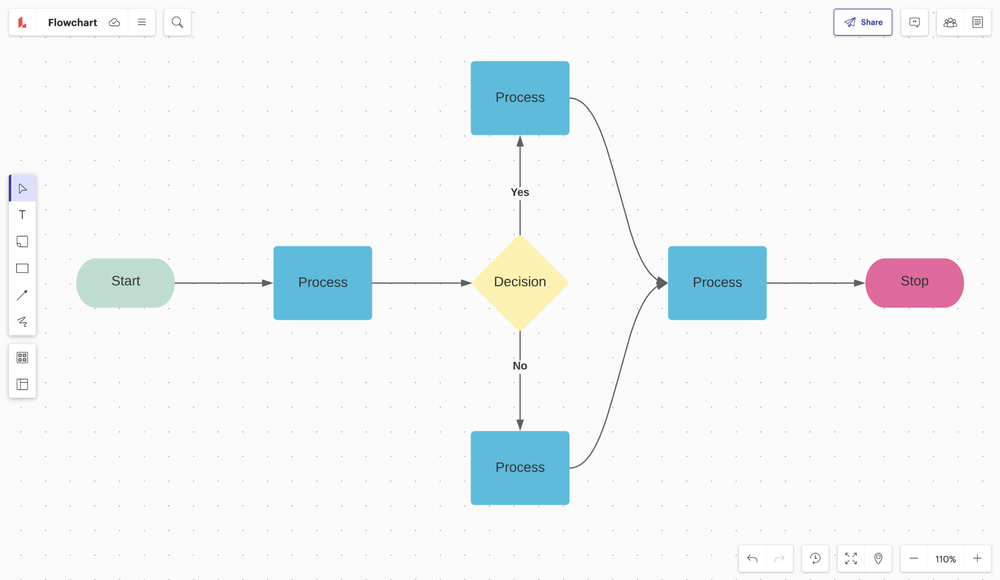
\includegraphics[scale=0.4]{exemplo_diagrama_de_fluxo.png}
	\caption[Exemplo de diagrama de fluxo]{Diagrama de fluxo. Fonte: \textcite{boyle1772}.}
	\label{fig:diagrama_fluxo}
\end{figure}

Paralelamente ao desenvolvimento do diagrama de fluxo, será criado um diagrama de classe \ref{fig:diagrama_classe}, definindo as diferentes classes de objetos que serão utilizados.

\begin{figure}[ht] 
	\centering
	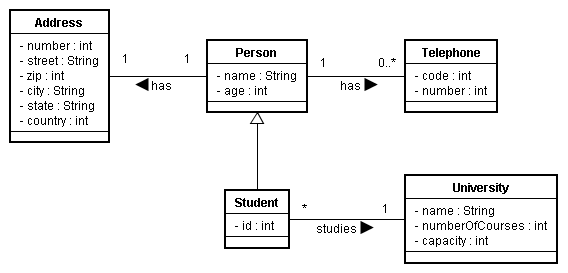
\includegraphics[scale=0.6]{exemplo_diagrama_de_classe.png}
	\caption[Exemplo de diagrama de classe]{Diagrama de classe. Fonte: \textcite{boyle1772}.}
	\label{fig:diagrama_classe}
\end{figure}

\newpage

Após a definição do design, com a criação do diagrama de fluxo e do diagrama de classe, inicia-se o processo de programação. A linguagem de programação Javascript será utilizada, juntamente com HTML e CSS. O desenvolvimento acompanhará o design pré-estabelecido. Com isso, espera-se a criação de um MVP (Minimum Viable Product).

Com a criação do MVP, em um ambiente local, a aplicação será hospedada em um servidor on-premisse da Universidade Federal de Ouro Preto. Após a hospedagem, espera-se que a aplicação esteja disponível para acesso público por meio da internet.


%link da imagem diagrama de fluxo: https://cdn-cashy-static-assets.lucidchart.com/marketing/pages/lucidspark/consideration/brainstorm-to-identify-each-part-of-your-workflow@2x@2x.png

% \textcolor{red}{Criar diagrama de fluxo com redes de Petri}

% Além do diagrama de fluxo, é necessária a criação de um diagrama de classe \ref{fig:diagrama_classe}. No diagrama de classe, define-se as diferentes classes de objeto que serão utilizados na aplicação. 

%Link da imagem diagrama de classe: https://www.researchgate.net/publication/228951230/figure/fig10/AS:349293408997379@1460289446190/Figura-11-Diagrama-de-classes-da-aplicacao-O-modelo-exibido-na-Figura-11-pode-ser-criado.png

% \textcolor{red}{Caso seja criado um banco de dados, explicar o seu funcionamento aqui}

% \textcolor{red}{Figuras de exemplo, substituir por imagem de melhor qualidade. Se possível, criar as próprias imagens}

%Falar sobre manuntenção da aplicação
%Falar sobre o estudo de softwares já existem

% \textcolor{red}{Novos tópicos serão abordados na metodologia. Muitas abordagens ainda não foram definidas. Ao longo do desenvolvimento, elas se tornarão mais claras }


% \section{Organização e estrutura}

% A estrutura e organização deve apresentar os assuntos abordados ao longo do seu texto. Por exemplo, no capítulo \ref{cap:revisao-de-literatura} são apresentados e discutidos os principais trabalhos neste campo de pesquisa. Já no capítulo \ref{cap:desenvolvimento}, que, por acaso, começa na página \pageref{cap:desenvolvimento}, o trabalho é desenvolvido.

% Um exemplo de tabela é apresentada na tabela~\ref{tab:001}. Você pode elaborar também tabelas online ou a partir de qualquer planilha eletrônica, inclusive em outros estilos, gerando o código em \LaTeX. Após isso, basta copiar e colar o código aqui. Um exemplo de site é o ``Tables Generator'': \url{http://www.tablesgenerator.com/}.

% % Please add the following required packages to your document preamble:
% % If you use beamer only pass "xcolor=table" option, i.e. \documentclass[xcolor=table]{beamer}
% \begin{table}[h]
% \centering
% \caption{Uma tabela}
% \label{tab:001}
% \resizebox{0.5\textwidth}{!}{%
% \begin{tabular}{|l|llllllllll|}
% \hline
%                                    & \multicolumn{10}{l|}{\cellcolor[HTML]{FF0000}\textbf{Meses}}                                                                                                                                                                         \\ \hline
% \cellcolor[HTML]{5EB91E}           & \multicolumn{1}{l|}{1} & \multicolumn{1}{l|}{2} & \multicolumn{1}{l|}{3} & \multicolumn{1}{l|}{4} & \multicolumn{1}{l|}{5} & \multicolumn{1}{l|}{6} & \multicolumn{1}{l|}{7}  & \multicolumn{1}{l|}{8} & \multicolumn{1}{l|}{9} & 10 \\ \hline
% \cellcolor[HTML]{5EB91E}\textbf{1} & \multicolumn{1}{l|}{}  & \multicolumn{1}{l|}{x} & \multicolumn{1}{l|}{}  & \multicolumn{1}{l|}{}  & \multicolumn{1}{l|}{}  & \multicolumn{1}{l|}{}  & \multicolumn{1}{l|}{}   & \multicolumn{1}{l|}{}  & \multicolumn{1}{l|}{}  &    \\ \hline
% \cellcolor[HTML]{5EB91E}\textbf{2} & \multicolumn{1}{l|}{x} & \multicolumn{1}{l|}{x} & \multicolumn{1}{l|}{}  & \multicolumn{1}{l|}{}  & \multicolumn{1}{l|}{}  & \multicolumn{1}{l|}{}  & \multicolumn{1}{l|}{xx} & \multicolumn{1}{l|}{}  & \multicolumn{1}{l|}{}  & x  \\ \hline
% \cellcolor[HTML]{5EB91E}\textbf{3} & \multicolumn{1}{l|}{}  & \multicolumn{1}{l|}{x} & \multicolumn{1}{l|}{}  & \multicolumn{1}{l|}{x} & \multicolumn{1}{l|}{}  & \multicolumn{1}{l|}{}  & \multicolumn{1}{l|}{}   & \multicolumn{1}{l|}{}  & \multicolumn{1}{l|}{}  &    \\ \hline
% \cellcolor[HTML]{5EB91E}\textbf{4} & \multicolumn{1}{l|}{}  & \multicolumn{1}{l|}{}  & \multicolumn{1}{l|}{}  & \multicolumn{1}{l|}{x} & \multicolumn{1}{l|}{}  & \multicolumn{1}{l|}{}  & \multicolumn{1}{l|}{xx} & \multicolumn{1}{l|}{}  & \multicolumn{1}{l|}{}  &    \\ \hline
% \cellcolor[HTML]{5EB91E}\textbf{5} & \multicolumn{1}{l|}{}  & \multicolumn{1}{l|}{}  & \multicolumn{1}{l|}{}  & \multicolumn{1}{l|}{}  & \multicolumn{1}{l|}{}  & \multicolumn{1}{l|}{}  & \multicolumn{1}{l|}{}   & \multicolumn{1}{l|}{}  & \multicolumn{1}{l|}{}  &    \\ \hline
% \cellcolor[HTML]{5EB91E}\textbf{6} & \multicolumn{1}{l|}{}  & \multicolumn{1}{l|}{}  & \multicolumn{1}{l|}{}  & \multicolumn{1}{l|}{}  & \multicolumn{1}{l|}{}  & \multicolumn{1}{l|}{}  & \multicolumn{1}{l|}{xx} & \multicolumn{1}{l|}{}  & \multicolumn{1}{l|}{}  &    \\ \hline
% \end{tabular}%
% }
% \end{table}

% Capitulo de revisão de literatura

\chapter{Fundamentação teórica} \label{cap:revisao-de-literatura}

% Um capítulo de revisão de literatura, também chamado de revisão teórica ou bibliográfica pode ser desenvolvido aqui. Procure dissertar sobre os autores e trabalhos mais relevantes em seu campo de estudo, em um diálogo com sua proposta. Um exemplo de citação em linha pode ser visto como em \textcite{Einstein1920}. 

% Um exemplo de citação do tipo autor-data pode também ser elaborado \cite{Einstein1920}. 

% Um exemplo de citação em nota de de rodapé, com notas explicativas pode ser visto aqui.\footcite[Esta nota vem antes.][p.~22]{descartes-carta-mersene} 

% Um outra outra forma de citação em nota explicativa pode ser elaborada\footnote{Escreva sua nota explicativa aqui, conforme \textcite{boyle1772}.}

% Um exemplo de citação direta pode ser feito. Conforme aconselha \textcite{boyle1772-a}:

% \begin{citacao}
% 	(...) Nam dui ligula, fringilla a, euismod sodales, sollicitudin vel, wisi. Morbi auctor lorem non justo. Nam lacus libero, pretium at, lobortis vitae, ultricies et, tellus. Donec aliquet, tortor sed accumsan bibendum, erat ligula aliquet magna, vitae ornare odio metus a mi. Morbi ac orci et nisl hendrerit mollis. Suspendisse ut massa. Cras nec ante. Pellentesque a nulla. Cum sociis natoque penatibus et magnis dis parturient montes, nascetur ridiculus mus. Aliquam tincidunt urna. Nulla ullamcorper vestibulum turpis. Pellentesque cursus luctus mauris.(...)
% \end{citacao}

\section{Redes de Petri}

As redes de Petri surgiram por volta da década de 1960 pela mente de Carl Adam Petri. Em 1962, Petri apresentou sua tese intitulada ``Kommunikation mit Automaten'', em que descreveu pela primeira vez a estrutura e funcionamento das redes de Petri. Esse nova ideia de representar sistemas permitiu a análise de sistemas concorrentes e paralelos.

Com o passar dos anos, a evolução tecnológica durante a terceira revolução industrial \cite{coutinho1992terceira} evidenciou os benefícios das redes de Petri, e sua aplicabilidade foi ampliada para além da modelagem de processos industriais, sendo adotada também para descrever processos dentro das áreas de Ciência da Computação e Engenharia de Software. Sendo assim, a partir dos anos de 1980, com o crescimento da automação industrial, as redes de Petri começaram a ser adaptadas para atender as necessidades de diferentes áreas. Com isso, surgiram as redes de Petri coloridas, as redes de Petri temporizadas e as redes de Petri estocásticas, como principais exemplos. 

\subsection*{O básico de redes de Petri}

Segundo \cite{CassandrasLafortune08}, uma rede de Petri clássica é representada graficamente por lugares, transições e arcos. Os lugares representam os estados do sistema, as transições indicam os eventos ou ações que podem ocorrer durante o funcionamento do sistema. Os arcos direcionados conectam os lugares as transições e as transições aos lugares. Essa estrutura permite a análise de propriedades importantes dos sistemas, como alcançabilidade, vivacidade, deadlock, reversibilidade, entre outras propriedades fundamentais para analise do comportamento de sistemas complexos. 

As redes de Petri seguem uma lógica matemática. Sendo assim, seus elementos são definidos como sendo:

\begin{equation*}
    \centering
    \left( P, T, A, w \right) \,,
    \label{elementos_rede_petri}
\end{equation*}
em que 

\textbf{$P = \left \{ p_{1},p_{2},...,p_{n} \right \}$} é o conjunto de lugares;

$T = \left \{ t_{1},t_{2},...,t_{n} \right \}$ é o conjunto de transições;

$A \subseteq \left ( P \times T \right ) \cup \left ( T \times P \right )$ representa os arcos de lugares para transições, e transições para lugares;

$w: A \rightarrow \left \{ 1,2,3,... \right \}$ é a função de peso dos arcos.

% Nas redes de Petri, pode-se ter diferentes formas de se interpretar os significados de seus elementos. Porém, de maneira geral, os lugares $P$ indicam os estados da representação. As transições $T$ indicam os eventos e, consequentemente, a mudança de estado da representação. Os pesos $w$ representam a condição necessária para o disparo de uma transição, ou seja, para a mudança de estado. Para isso, a quantidade mínima de tokens presentes em um lugar $P$ necessita ser igual, ou superior, ao peso do arco. E os tokens, por fim, representam a quantidade de elementos presentes em um lugar $P$.

Com tais elementos torna-se possível a criação e modelagem de redes de Petri para a representação de sistemas concorrentes. Conforme o exemplo \ref{exemplo_rede_petri_simples} é possível evidenciar uma rede de Petri simples, permitindo a compreensão de sua estrutura e funcionamento das redes de Petri em um âmbito geral.

\begin{exemplo}[Uma rede de Petri simples]
\label{exemplo_rede_petri_simples}]

Inicialmente, define-se os conjuntos $P, T, A, w$. 
\begin{eqnarray*}
P &=& \left \{ p_{1},p_{2}\right \} \\
T &=& \left \{ t_{1}\right \} \\
A &=& \left \{ \left (p_{1},t_{1}\right ),\left (t_{1},p_{2}\right ) \right \} \\
w\left ( p_{1},t_{1} \right ) &=& 2 \\
w\left ( t_{1},p_{2} \right ) &=& 1 \\
\end{eqnarray*}
\end{exemplo}
%
Para esse exemplo, tem-se os lugares $p_{1}$ e $p_{2}$. O arco $\left ( p_{1},t_{1} \right )$ conecta o lugar $p_{1}$ a transição $t_{1}$, e seu peso $w\left ( p_{1},t_{1} \right )$ é igual a 2.O arco $\left ( t_{1},p_{2} \right )$ conecta a transição  $t_{1}$ ao lugar $p_{2}$, e seu peso $w\left ( t_{1},p_{2} \right )$ é igual a 1. 

Tendo a lógica matemática definida, pode-se ilustrar graficamente a mesma rede de Petri, conforme a figura \ref{fig:rede_petri_simples_ex_01}.

\begin{figure}[ht] 
	\centering
	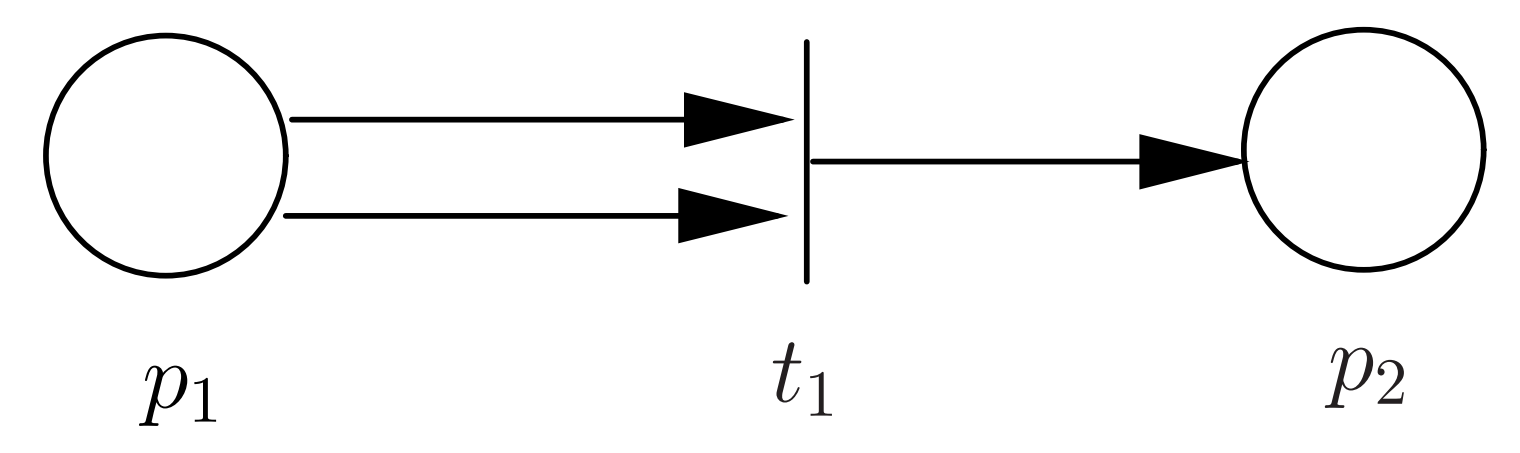
\includegraphics[scale=0.3]{exemplo_simples_rede_petri.png}
	\caption[Rede de Petri Simples]{Rede de Petri Simples. Fonte: \textcite{CassandrasLafortune08}.}
	\label{fig:rede_petri_simples_ex_01}
\end{figure} 

Para a mudança de estado dessa representação é necessário, no mínimo, duas marcações no lugar $p_{1}$. Com essa condição satisfeita, a transição $t_{1}$ passa a estar habilitada, tornando possível a mudança de estado, como ilustrado na figura \ref{fig:rede_petri_simples_ex_02}.

\newpage

\begin{figure}[ht] 
	\centering
	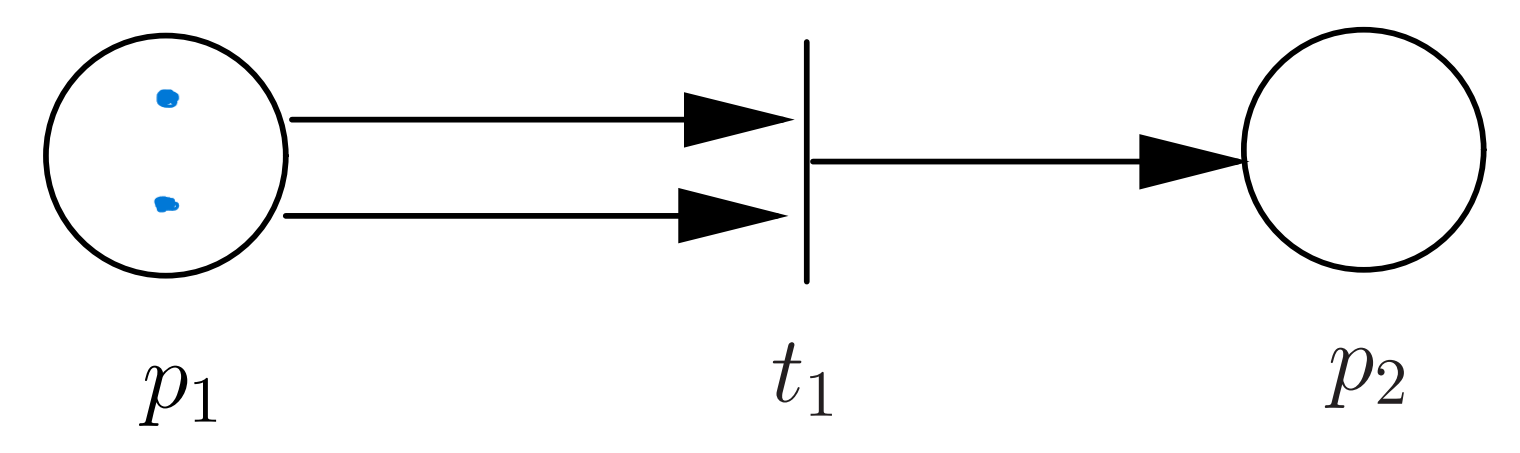
\includegraphics[scale=0.3]{exemplo_simples_rede_petri_marcacao_p1.png}
	\caption[Rede de Petri Simples]{Transição $t_{1}$ habilitada. Fonte: \textcite{CassandrasLafortune08}.}
	\label{fig:rede_petri_simples_ex_02}
\end{figure}

Após a execução da transição $t_{1}$, as duas marcações em $p_{1}$ somem, e uma marcação em $p_{2}$ surge. Essa lógica se dá por meio do peso dos arcos. O arco $(p_{1},t_{1})$, anterior a transição $t_{1}$ possui peso 2, logo o lugar $p_{1}$ cede duas marcações para a transição $t_{1}$ ocorrer. De forma análoga, o lugar $p_{2}$ ganha uma marcação, pois o arco $(t_{1},p_{2})$, posterior a transição $t_{1}$, tem peso igual a 1. Essa lógica é ilustrada pela figura \ref{fig:rede_petri_simples_ex_03}.

\begin{figure}[ht] 
	\centering
	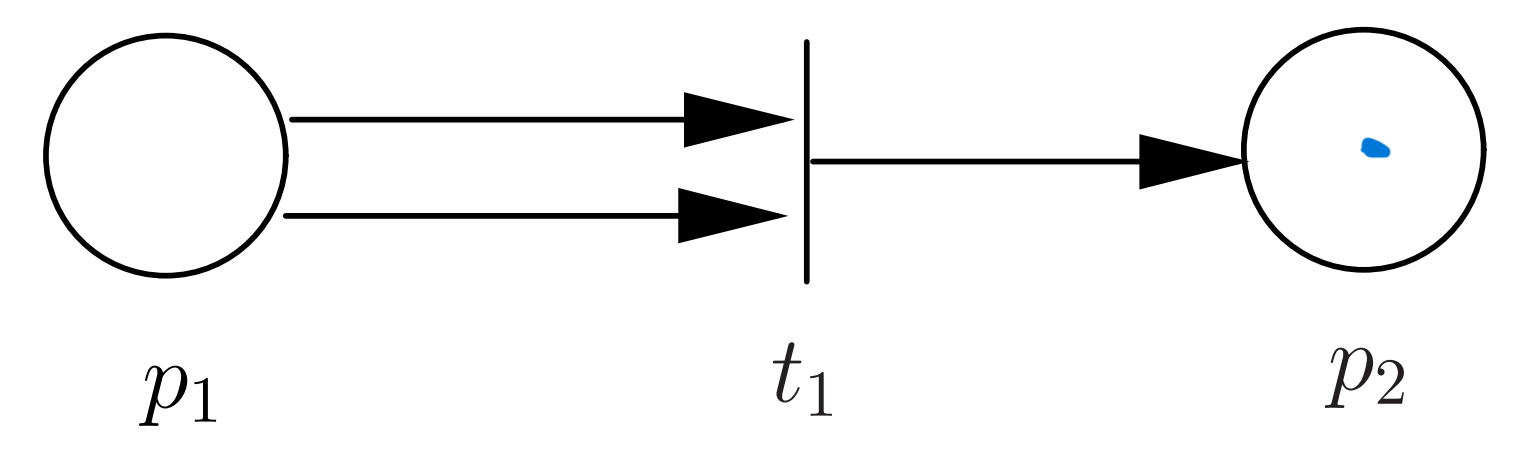
\includegraphics[scale=0.3]{exemplo_simples_rede_petri_marcacao_p2.png}
	\caption[Rede de Petri Simples]{Rede de Petri após a transição $t_{1}$ ter sido executada. Fonte: \textcite{CassandrasLafortune08}.}
	\label{fig:rede_petri_simples_ex_03}
\end{figure}

%\end{exemplo}

Com o exemplo \ref{exemplo_rede_petri_simples}, é possível entender o princípio básico de funcionamento das redes de Petri. Dessa forma, tem-se que:

 \begin{enumerate}[label=(\alph*)]
    \item \textbf{habilitação de uma transição:} para a habilitação de uma transição $t_{i}$ é necessário que o número de marcações associados ao lugar $p_{i}$, anterior a transição, seja igual, ou superior, ao peso do arco que conecta o lugar $p_{i}$ a transição $t_{i}$;
    \item \textbf{peso dos arcos:} ...;
    \item \textbf{movimentação das marcações:} ....
\end{enumerate}


\begin{exemplo} \textbf{Uma rede de Petri mais desenvolvida}
\label{exemplo_rede_petri_desenvolvidada}

\end{exemplo}

A lógica utilizada nas redes de Petri podem facilmente ser traduzidas para os modelos utilizados na lógica de programação Ladder, uma vez que as redes de Petri também se utilizam da álgebra booleana. 

%\begin{exemplo} \textbf{A mesma representação em rede de Petri e Lader}
    
%\end{exemplo}

% \textcolor{red}{Trocar imagens das redes de Petri por imagens retiradas da minha própria aplicação.}

\subsection*{Variantes das redes de Petri clássica}

Além da rede de Petri clássica, com o passar dos anos, e com o avanço da tecnologia, houve a necessidade de se adaptar as redes de Petri para atender cenários mais realistas e completos. A partir dessas variações, três delas se destacam, sendo elas as redes de Petri Temporizadas \ref{exemplo_temporarizada}, Coloridas \ref{exemplo_colorida} e Estocásticas \ref{exemplo_estocastica}. Cada uma delas, permite uma representação mais abrangente dos sistemas do mundo real, pois permitem o desenvolvimento de aspectos como tempo, características distintas e incertezas que compõem os diversos tipos de sistemas.


\subsubsection*{Temporizada}

\textcolor{red}{referenciar o artigo dcce.ibilce.unesp.br/~aleardo/cursos/str/cap3.pdf }

As redes de Petri Temporizadas surgiram a partir da necessidade de se atribuir uma propriedade temporal a certos atributos de um sistema. Ao contrário das redes de Petri clássicas, que consideram as transições como instantâneas, as redes de Petri Temporizadas reconhecem que uma vasta quantidade de sistemas do mundo real estão intrinsecamente ligados a variáveis de tempo. Tal fato é extremamente relevante, já que a maiorias dos eventos nesses sistemas demanda certo período de tempo para sua execução completa.

Nas redes de Petri Temporizadas, pode-se considerar dois cenários para a associação de variáveis de tempo. No primeiro cenário, se tem a associação de tempo $C_{i}$ a duração de uma certa transição $t_{i}$. Ou seja, o evento representado pela transição terá um intervalo de tempo para ser executado. No segundo cenário, associa-se a variável de tempo $C_{i}$ aos lugares $p_{i}$. Dessa forma, as marcações tornam-se disponíveis apenas após o intervalo de tempo. Define-se assim: 

\begin{itemize}
        \item Tempo $C_{i}$ associado a transição $t_{i}$;
        \item Tempo $C_{i}$ associado ao lugar $p_{i}$.
\end{itemize}

As transições temporizadas, nos modelos gráficos, para se diferenciar das transições instantâneas, possuem uma cor associada diferente, e isso pode ser evidenciado na maioria dos softwares já disponíveis. Enquanto as transições instantâneas possuem fundo preto, as transições temporárias possuem fundo branco. Além disso, quando uma transição estiver disponível para o disparo, ela possuirá fundo vermelho, conforme a figura \ref{fig:cores_transição}. 

\begin{figure}[ht] 
	\centering
	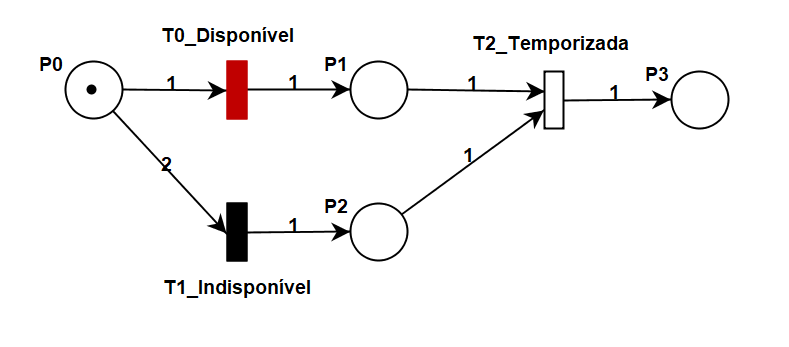
\includegraphics[scale=0.75]{figuras/exemplo_cores_transicao.png}
	\caption[Cores dos tipos de transição]{Cores dos tipos de transição. Fonte: Pipe.}
	\label{fig:cores_transição}
\end{figure}

No exemplo \ref{exemplo_temporarizada} há uma transição fonte $t_{0}$, que está sempre habilitada, ligada a posição $p_{0}$. O lugar $p_{0}$ está ligado a uma transição temporizada $t_{1}$, por meio de um arco $w(p_{0},t_{1})$ de peso 2. Além disso, a transição $t_{1}$ possui um tempo $C_{1}$ associado. Ou seja, após o disparo da transição $t_{1}$, haverá um tempo $C_{1}$ de espera, indicando o tempo de execução do evento associado a transição. Após a decorrência desse tempo, duas marcações, associadas ao lugar $p_{0}$, se transformarão em apenas uma marcação no lugar $p_{1}$.  

\begin{exemplo} \textbf{Temporizada}
\label{exemplo_temporarizada}

\begin{figure}[ht] 
	\centering
	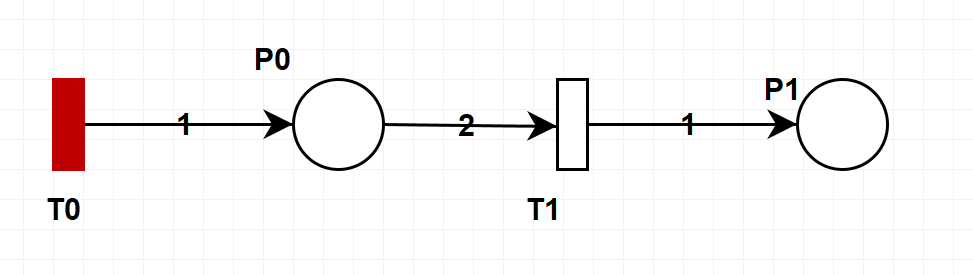
\includegraphics[scale=0.55]{figuras/exemplo_rede_petri_temporizada_1.png}
	\caption[Rede de Petri Temporizada - Estágio 1]{Rede de Petri Temporizada - Estágio 1. Fonte: Pipe.}
	\label{fig:rede_petri_temporizada_ex_01}
\end{figure}

\begin{figure}[ht] 
	\centering
	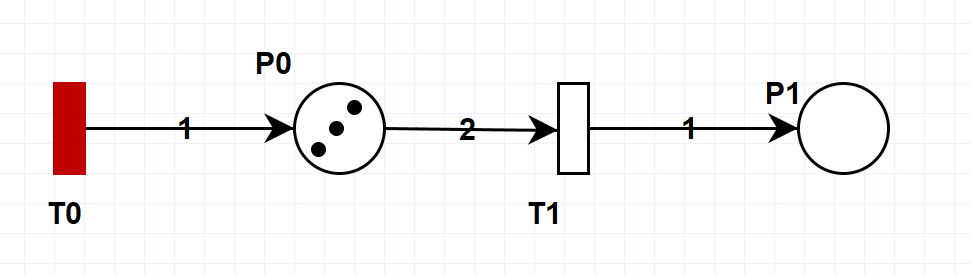
\includegraphics[scale=0.55]{figuras/exemplo_rede_petri_temporizada_2.png}
	\caption[Rede de Petri Temporizada - Estágio 2]{Rede de Petri Temporizada - Estágio 2. Fonte: Pipe.}
	\label{fig:rede_petri_temporizada_ex_02}
\end{figure}

\begin{figure}[ht] 
	\centering
	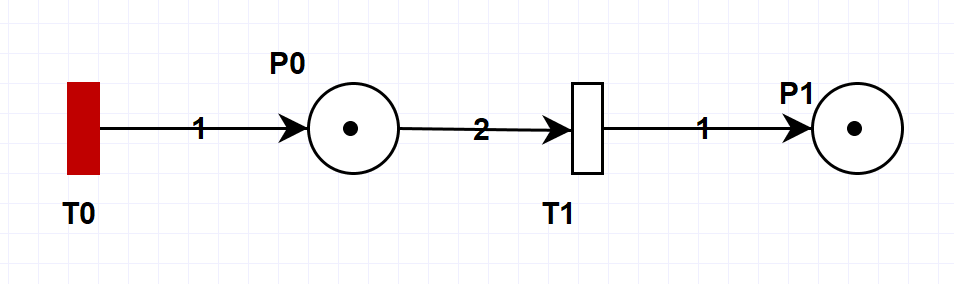
\includegraphics[scale=0.55]{figuras/exemplo_rede_petri_temporizada_3.png}
	\caption[Rede de Petri Temporizada - Estágio 3]{Rede de Petri Temporizada - Estágio 3. Fonte: Pipe.}
	\label{fig:rede_petri_temporizada_ex_03}
\end{figure}

\end{exemplo}

\subsubsection*{Colorida}

As redes de Petri Coloridas surgiram com a ideia de diminuir o tamanho das representações \cite{frances2003introduccao}, uma vez que muitas representações contam com ideias semelhantes. Através da individualização das marcações, os processos e recursos de um sistema podem agora representar diferentes ideias em uma mesma rede, ou parte dela. O termo "colorida" surge da ideia de termos marcações, com diferentes cores, representando diferentes recursos. Essa forma de representação tem como principal benefício reduzir o tamanho e, consequentemente, a complexidade da representação em uma rede de Petri. Comparando os exemplos, consegue-se analisar tal propriedade. Ambas as redes representam a mesma ideia, porém na segunda representação temos uma quantidade menor de elementos, o que facilita o entendimento. 

Uma vez que se consegue representar as marcações com diferentes cores, torna-se mais simples a representação de sistemas complexos, diminuindo a complexidade das análises. Nas redes de Petri tradicionais, cada lugar representa um único estado do sistema representado. As redes de Petri coloridas deixam de forma mais intuitiva e clara a representação de múltiplos estados ou recursos. 

\begin{exemplo} \textbf{Colorida}
\label{exemplo_colorida}

\end{exemplo}

\subsubsection*{Estocásticas}

Uma rede de Petri estocástica é mais uma variação das redes de Petri clássicas. Enquanto as redes de Petri clássicas são frequentemente usadas para representar sistemas discretos e determinísticos, as redes de Petri estocásticas permitem incorporar a aleatoriedade e a incerteza na representação.

Nas redes de Petri estocásticas, os elementos básicos, como lugares, transições e arcos, são semelhantes aos das redes de Petri convencionais. No entanto, a principal diferença é que as transições não são ativadas de forma determinística, mas sim com base em probabilidades. Isso significa que a ocorrência de uma transição é governada por um processo estocástico, como um processo de Poisson, e a escolha de qual transição ocorre em um determinado momento é determinada por probabilidades.

Essa abordagem estocástica é especialmente útil para modelar sistemas onde eventos ocorrem de maneira aleatória, como sistemas de comunicação, sistemas biológicos e sistemas de manufatura com variações de tempo e recursos. As redes de Petri estocásticas permitem a análise de propriedades estatísticas do sistema, como a probabilidade de estados específicos serem alcançados ou a distribuição de tempo entre eventos.

Conforme o exemplo \ref{exemplo_estocastica} é possível analisar o funcionamento de uma rede de Petri estocástica.

\textcolor{red}{Criar exemplo de Rede de Petri estocástica}

\begin{exemplo} \textbf{Estocásticas}
\label{exemplo_estocastica}

\end{exemplo}

%\section{Linguagens de marcação de texto}

\section{Tecnologias para o desenvolvimento web} \label{cap:tecnologiaweb}

O desenvolvimento de aplicações web interativas e eficientes requer a utilização de um conjunto de tecnologias modernas que, utilizadas juntas, fornecem os recursos necessários para a construção de interfaces gráficas, implementação de lógicas, estilização visual e versionamento de código. Para tais necessidades, tem-se as principais ferramentas utilizadas para tais finalidades, sendo elas o HTML, CSS, Javascript e Git. 

\subsection*{HTML}

O \textbf{HTML} (\textit{HyperText Markup Language}) é a linguagem de marcação padrão para a criação e estruturação de conteúdo na internet \cite{mdn_html}. Sua função principal é definir a estrutura semântica de uma página web, organizando elementos como títulos, parágrafos, imagens, links, botões, formulários e vários outros elementos. No desenvolvimento de uma aplicação web para construção e simulação de redes de Petri, o HTML atua como esqueleto da interface, definindo todas as funcionalidades com as quais o usuário teria acesso. 
  
Dessa forma, o HTML é composto por uma série de elementos conhecidos como \textit{tags}, os quais são utilizados para estruturar e identificar semanticamente o conteúdo de uma página web. Cada {\textit{tag}} possui uma função específica e pode conter atributos que modificam seu comportamento ou aparência.

A estrutura básica de um documento HTML é hierárquica e inicia com a \textit{tag} \textbf{<!DOCTYPE html>}, seguida pelas \textit{tags} \textbf{<html>}, \textbf{<head>} e \textbf{<body>}, que organizam o conteúdo e os metadados da página. O conteúdo visual e interativo apresentado ao usuário reside, predominantemente, dentro da \textit{tag} \textbf{<body>}, enquanto elementos de configuração, definição de estilos e \textit{scripts} são alocados na \textit{tag} \textbf{<head>}. 

Por fim, através do arquivo HTML faz-se a junção de outras tecnologias, tais como o CSS e o Javascript. 

\subsection*{CSS}

O \textbf{CSS} (\textit{Cascading Style Sheets}) é a linguagem responsável pela definição da aparência dos elementos HTML \cite{mdn_css}. Através do CSS, é possível personalizar cores, tamanhos, posicionamentos, margens, fontes e efeitos visuais. A estilização também contribuiu para a experiência do usuário ao proporcionar \textit{feedback} visual em interações, como a mudança de cor de um botão ao clicar e a exibição de mensagens de alerta. 

Para a aplicação de construção e simulação de redes de Petri, o CSS é fundamental para estilizar os elementos gráficos, os lugares, transições e arcos, definindo as cores e tamanhos, e organizando o layout da área de desenho e dos painéis de controle, garantindo uma experiência de usuário intuitiva e esteticamente agradável. 

\subsection*{Javascript}

O \textbf{Javascript} é uma linguagem de programação interpretada, executada no lado do navegador do usuário, e é responsável por implementar comportamentos dinâmicos nas páginas web \cite{mdn_css}. Trata-se de uma linguagem orientada a eventos, que permite responder a interações do usuário, manipular o \textit{DOM} em tempo real, controlar estados da aplicação e realizar operações lógicas e matemáticas.

Enquanto o HTML é responsável pela estrutura da página e o CSS pela sua apresentação visual, o Javascript permite a implementação de comportamentos dinâmicos, como respostas a eventos de usuários, manipulação do conteúdo da página em tempo real, validação de formulários, animações, chamadas assíncronas, entre outros. 

Na aplicação proposta, o Javascript desempenha papel central no funcionamento do simulador. Toda a lógica de construção e simulação da rede de Petri foi implementada em Javascript, permitindo o desenvolvimento de diversas funcionalidades para a aplicação e para o cumprimento dos objetivos específicos do projeto \ref{cap:objEspecifico}. 

\subsection*{Git} \label{cap:git}

O \textbf{Git} é um sistema de controle de versão distribuído amplamente utilizado em projetos de desenvolvimento de software \cite{git_docs}. Seu principal objetivo é registrar e gerenciar o histórico de alterações feitas no código-fonte, permitindo o acompanhamento da evolução do projeto, reversão de modificações e colaboração de forma eficiente.

Para o desenvolvimento do projeto, o controle de versão é essencial. O Git, em conjunto com a plataforma GitHub, permitem não apenas o versionamento contínuo do código-fonte, mas também a criação de ramificações para o desenvolvimento simultâneo de diferentes funcionalidades, sem comprometer a integridade da versão principal do projeto. Além disso, o GitHub viabiliza a disponibilização pública do repositório, favorecendo a transparência, a colaboração e o acesso ao código por terceiros. A utilização de ambas ferramentas garantem a preservação do histórico de alterações, facilitando o rastreamento de modificações, a identificação de regressões e a reversão de mudanças indesejadas, contribuindo significativamente para a organização e segurança do desenvolvimento.

\section{Simuladores Conhecidos}

\subsection*{Pipe}

O \textbf{PIPE} (Plataform Independent Petri Net Editor) é uma ferramenta de software de código aberto para simulação e análise de redes de Petri \cite{Dingle2009PIPE2}. Desenvolvido em linguagem Java, o PIPE se destaca por ser uma ferramenta multiplataforma, operando  em diversos sistemas operacionais, como Windows, MacOS e Linux, facilitando sua acessibilidade e disseminação na comunidade acadêmica e de pesquisa. Entretanto, o projeto aparenta não estar mais em desenvolvimento, visto que, não há mais contribuições no repositório do projeto no Github \cite{PIPEGitHub}. 

\begin{figure}[ht] 
	\centering
	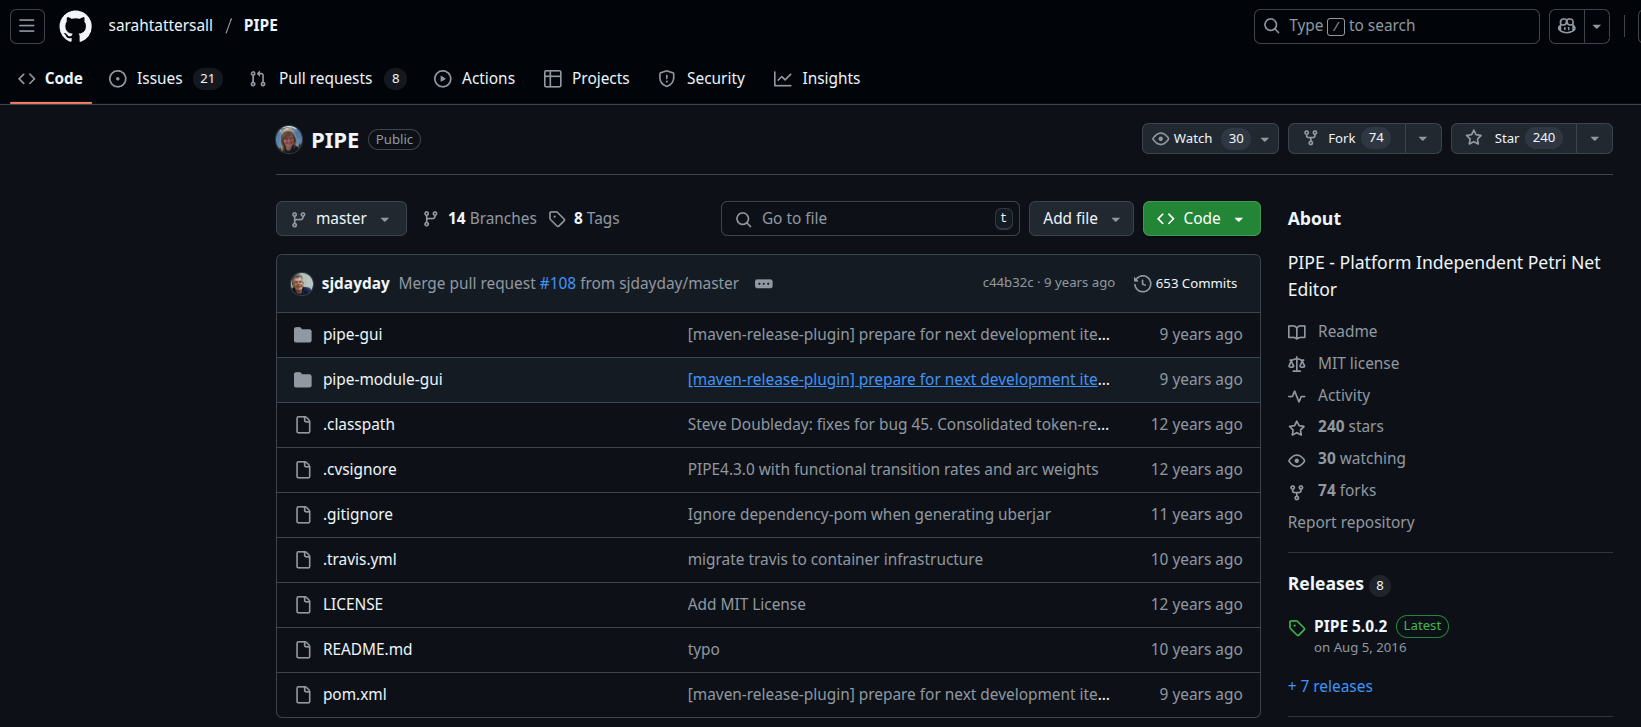
\includegraphics[scale=0.30]{figuras/pipeRepo.png}
	\caption[Repositório no Github do PIPE]{Repositório no Github do PIPE}
	\label{fig:pipeRepo}
\end{figure}
\FloatBarrier

\begin{figure}[ht] 
	\centering
	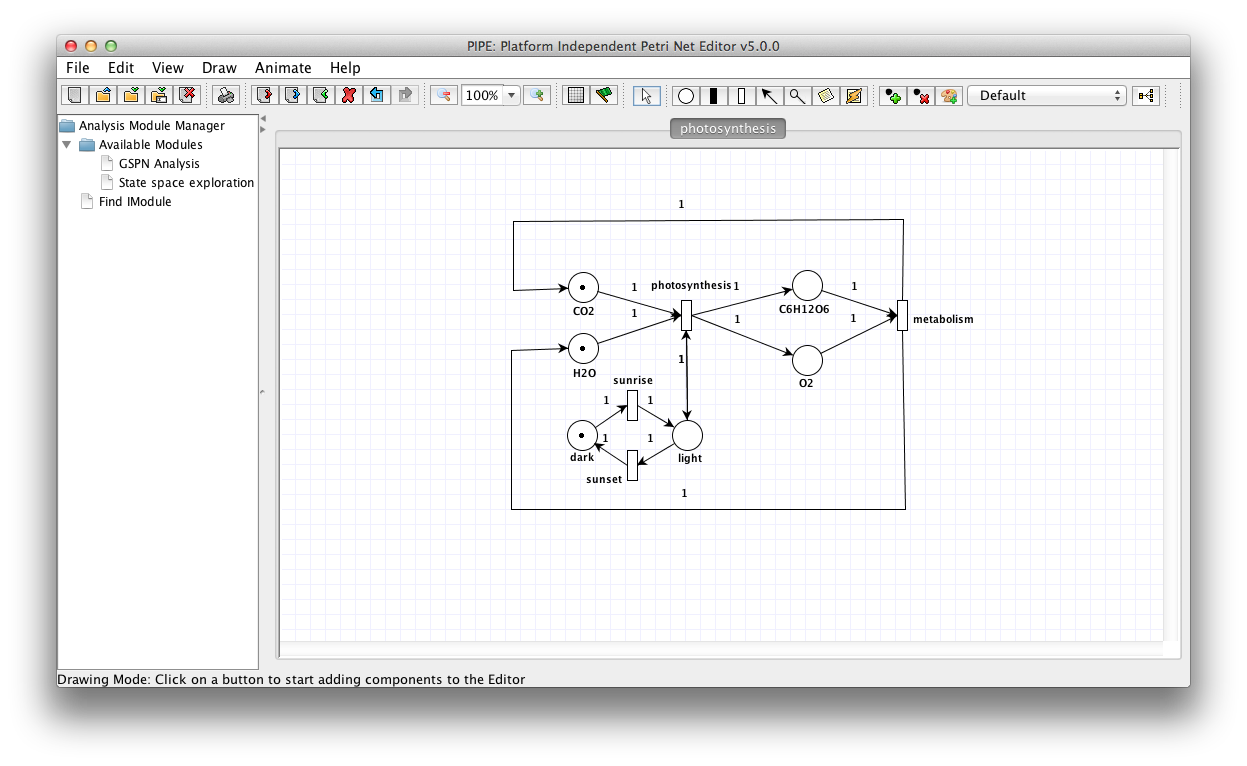
\includegraphics[scale=0.30]{figuras/pipe.png}
	\caption[Interface do simulador PIPE]{Interface do simulador PIPE}
	\label{fig:interfacePipe}
\end{figure}
\FloatBarrier

Apesar do PIPE ser uma excelente ferramenta para modelagem e simulação de redes de Petri, seu projeto aparenta não ter mais atualizações, e sua instalação requer conhecimento técnico em Java, podendo ser impeditivo para alguns usuários. Além disso, sua última versão apresenta \textit{bugs}, dificultando a sua utilização. 

\subsection*{APO}

A ferramenta APO (Accessible Petri Net Operations) consiste em uma interface web desenvolvida para facilitar o uso do APT (Analysis of Petri Nets and Transition Systems), um software robusto voltado à análise e síntese de redes de Petri e Sistemas de Transição \cite{apoGithub}. 

\begin{figure}[ht] 
	\centering
	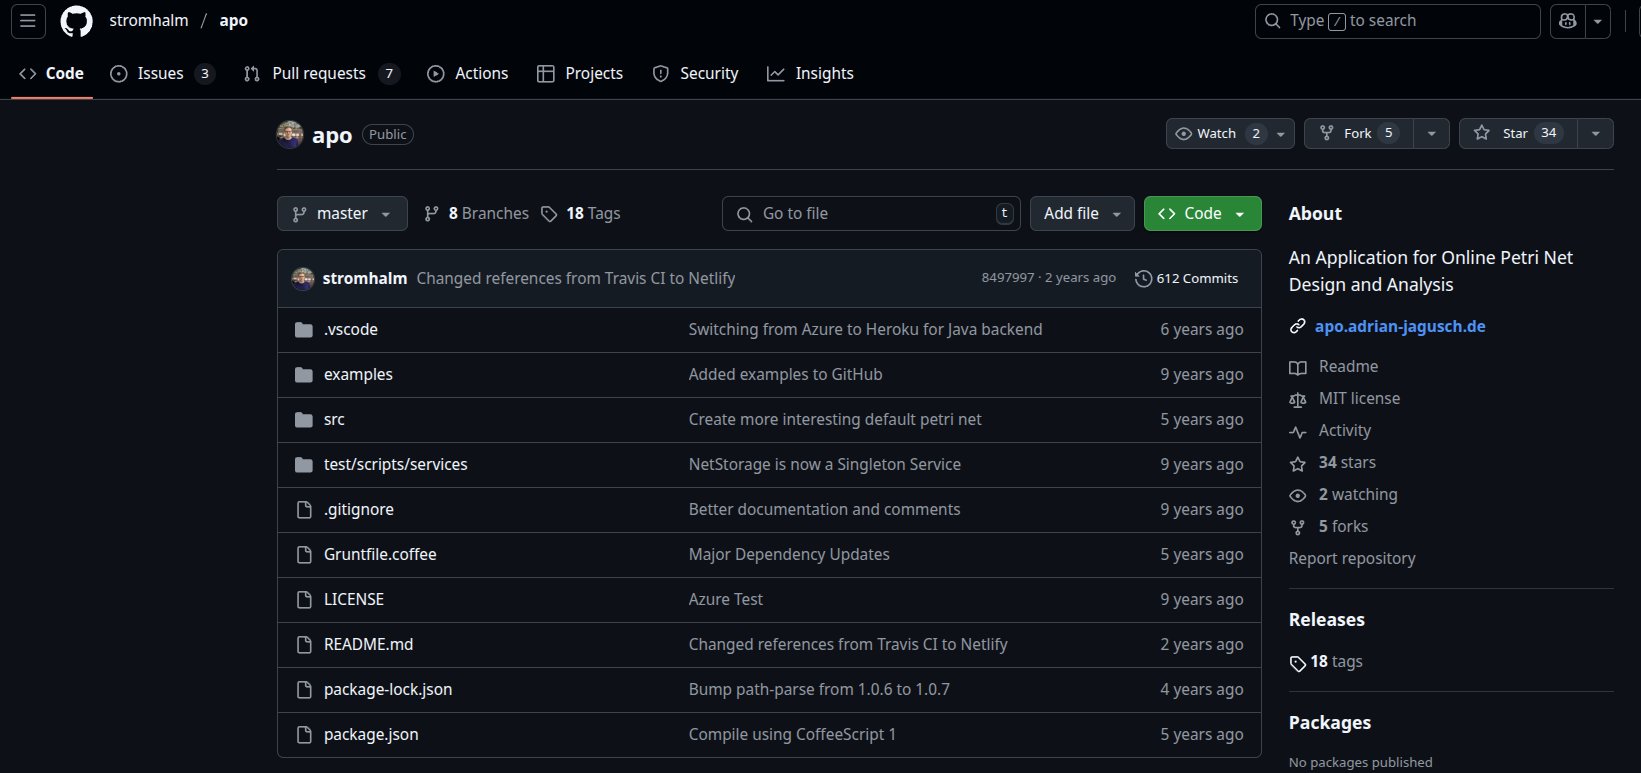
\includegraphics[scale=0.30]{figuras/apoRepo.png}
	\caption[Repositório no Github do APO]{Repositório no Github do APO}
	\label{fig:pipeAPO}
\end{figure}
\FloatBarrier

\begin{figure}[ht] 
	\centering
	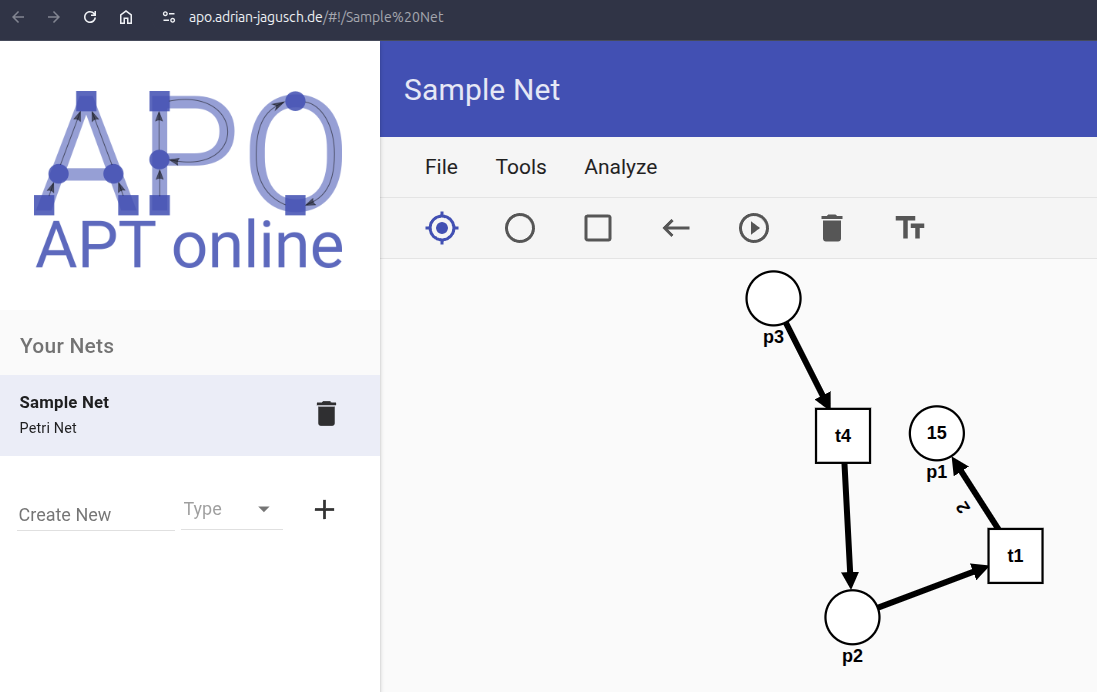
\includegraphics[scale=0.30]{figuras/apoInterface.png}
	\caption[Interface do simulador APO]{Interface do simulador APO}
	\label{fig:interfaceAPO}
\end{figure}
\FloatBarrier

A construção das redes é feita de maneira interativa, por meio de uma barra de ferramentas intuitiva, que permite a criação de lugares, transições e arcos. Após a modelagem da rede, é possível realizar análises automáticas utilizando os algoritmos integrados ao APT, diretamente acessíveis por meio da barra de menu. 

\subsection*{TryRdP}

O \textbf{TryRdP} é uma ferramenta web gratuita e interativa desenvolvida com o objetivo de apoiar o ensino e a aprendizagem significativa das redes de Petri \cite{educomp}. Diante da dificuldade que muitos estudantes enfrentam com o ensino tradicional, muitas vezes excessivamente teórico e abstrato, o TryRdP surge como uma alternativa mais prática e acessível, oferecendo uma abordagem baseada em exemplos reais de aplicação. 

A ferramenta é organizada em três seções principais: introdução, modelagem básica e modelagem avançada, cada uma com explicações detalhadas dos conceitos e exercícios que aumentam progressivamente em complexidade. Essa estrutura favorece o aprendizado gradual e autônomo, permitindo que os usuários desenvolvam suas habilidades de forma prática e contextualizada. Além disso, a ferramenta TryRdP foi desenvolvida utilizando-se de tecnologias web modernas, como HTML, CSS e JavaScript, além de outros \textit{frameworks} para desenvolvimento web.

\begin{figure}[ht] 
	\centering
	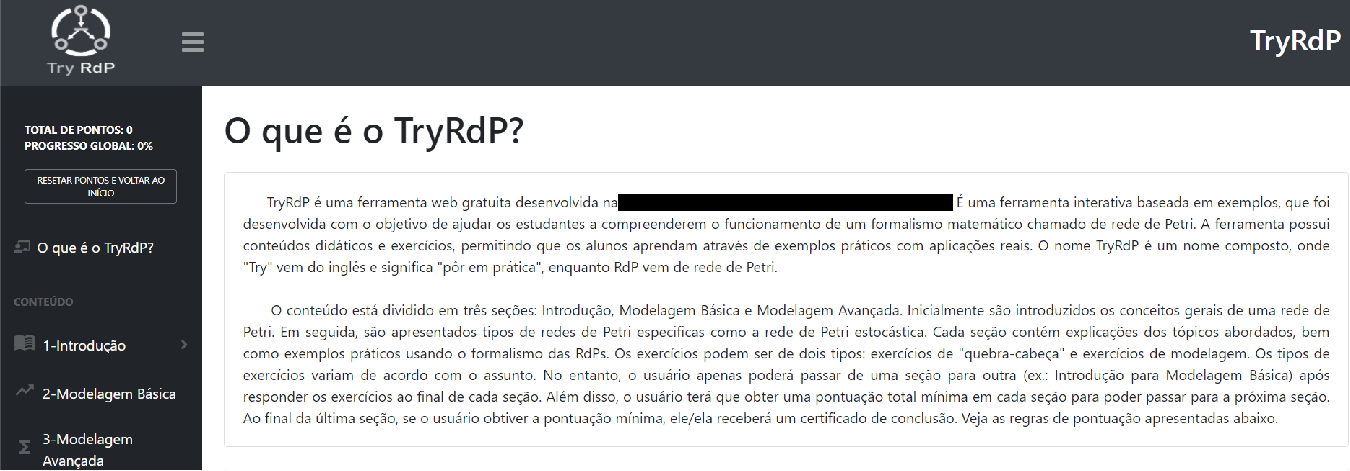
\includegraphics[scale=0.40]{figuras/tryrdpInterface.png}
	\caption[Interface do simulador TryRdP]{Interface do simulador TryRdP}
	\label{fig:interfaceTryRdP}
\end{figure}
\FloatBarrier

O TryRDP configura-se como uma ferramenta bastante eficaz para fins educacionais, especialmente no processo de aprendizagem sobre redes de Petri. Sua proposta se destaca pela disponibilização de exercícios com níveis de dificuldade progressivos, além de fornecer mensagens de \textit{feedback} e correção sempre que o usuário comete erros, o que contribui significativamente para o aprendizado ativo. No entanto, a acessibilidade da ferramenta ainda representa uma limitação, uma vez que a localização do endereço \textit{URL} para acesso externo não é intuitiva nem prontamente disponível, dificultando seu uso por novos usuários.

% ---
\chapter{Desenvolvimento} \label{cap:desenvolvimento}

O desenvolvimento deste projeto iniciou-se com uma análise geral das funcionalidades centrais que a aplicação web deveria atender para alcançar seus objetivos. Desde o princípio, buscou-se criar uma ferramenta funcional e intuitiva que permitisse aos usuários construir, visualizar e simular redes de Petri. Essas funcionalidades formam a espinha dorsal da aplicação, garantindo não apenas o cumprimento do objetivo principal, mas também estabelecendo uma base sólida para futuras expansões e melhorias. Dessa forma, o sistema foi pensado para ser escalável, possibilitando a adição de novas funcionalidades e o aprimoramento contínuo da interface e da experiência do usuário. Essas funciolidades buscam cumprir os seguintes requisitos: 

\begin{enumerate}
	\item Definição de um espaço na tela para a criação de uma rede Petri;
	\item Capacidade de adição dos elementos que compõem uma rede de Petri;
	\item Capacidade de renderização dos elementos na tela;
	\item Capacidade de movimentação dos elementos adicionados a área destinada ao desenvolvimento da rede de Petri;
	\item Uma vez criado um elemento, ser possível modificar suas propriedades;
	\item Possibilidade de exclusão dos elementos, tanto de forma individidual, quanto de modo geral;
	\item Possibilidade de salvar e carregar as redes de Petri criadas;
	\item Possibilidade de simular a rede de Petri desenvolvida;
	\item Forma de hospedar a aplicação de modo online para acesso via navegador de internet.
\end{enumerate}

Com os requisitos em mente, criou-se a base de arquivos que seriam utilizados para o desenvolvimento da aplicação web, sendo eles: 

\begin{enumerate}
	\item index.hmtl;
	\item style.css;
	\item script.js.
\end{enumerate}

Através do arquivo \textbf{index.html} estruturou-se toda a interface da aplicação. É nele em que se define todos os elementos que vão fazer parte da interface apresentada ao usuário final. O arquivo \textbf{sytle.css} define as principais propriedades visuais que foram estabelicidas anteriormente no arquivo \textbf{index.html}. Por fim, no arquivo \textbf{script.js} se define toda a lógica da aplicação. Através da liguagem de programação Javascript se desenvolveu todas as funcionalidades que foram estabelicidas anteriormente. 

No arquivo \textbf{index.hmtl} inicialmente foi criado o título da página denominado \textbf{Online Petri Net Simulator} e seu posicionamento foi definido no topo e ao centro da tela, conforme imagem abaixo:

\begin{figure}[ht] 
	\centering
	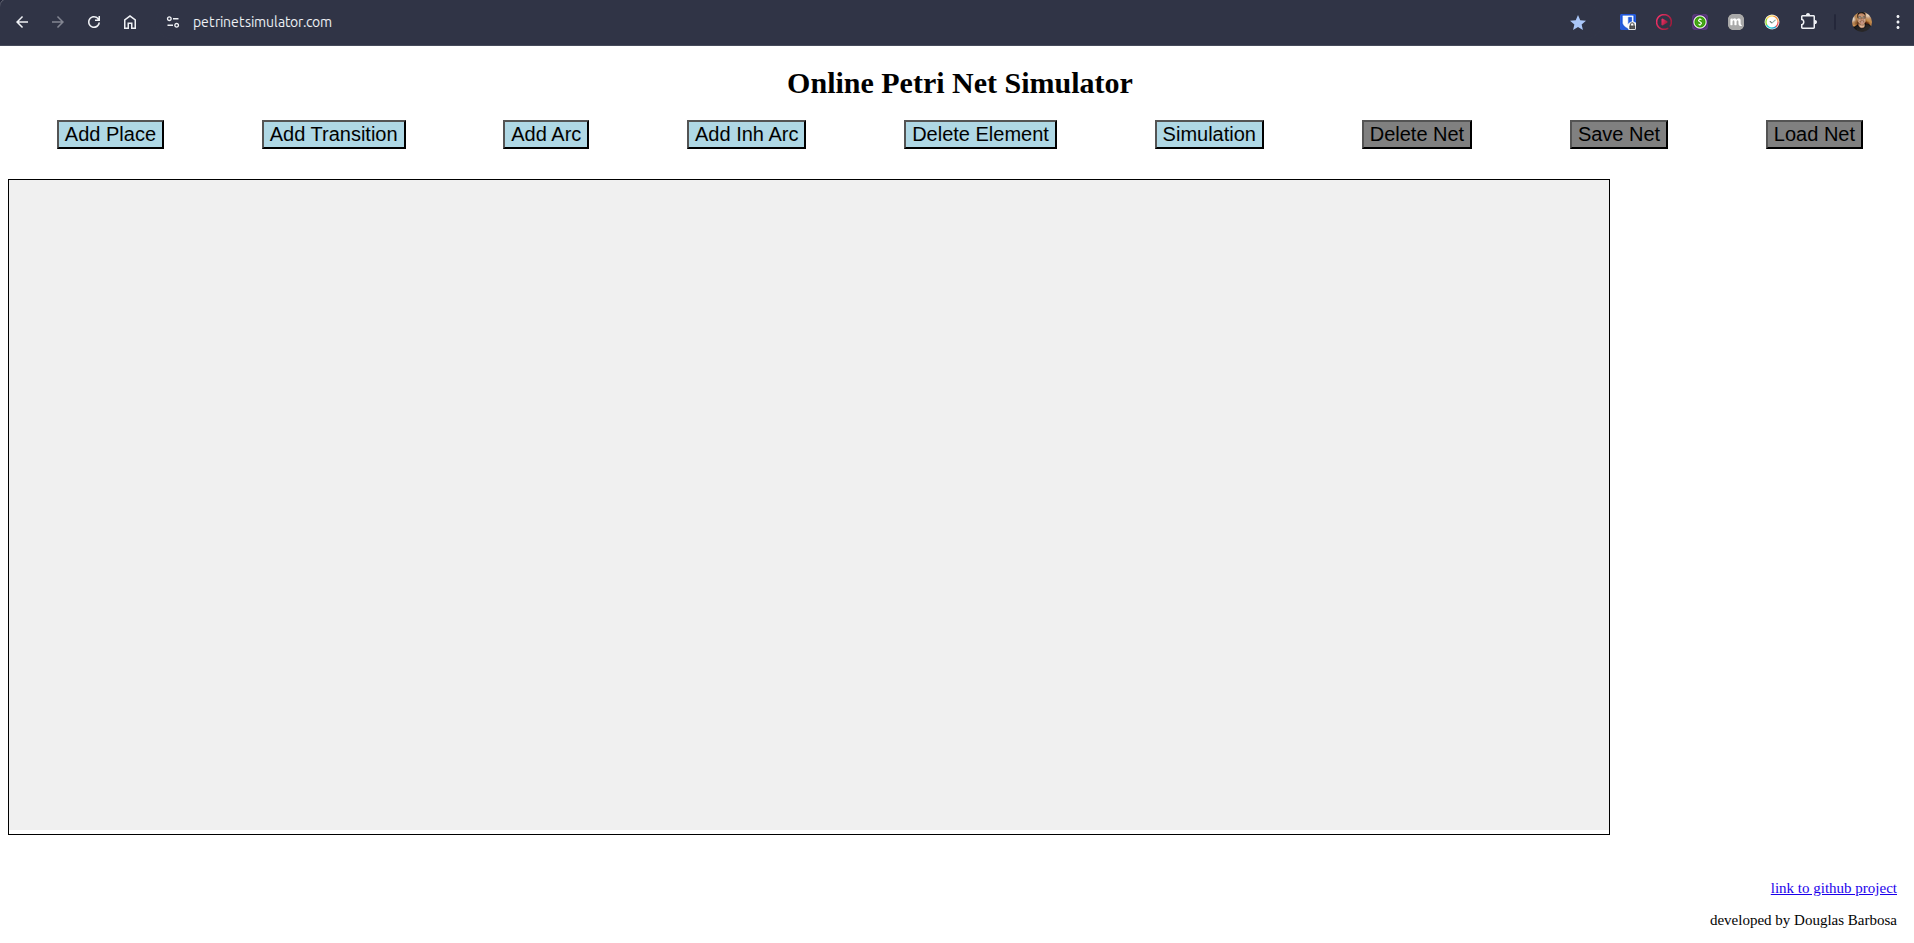
\includegraphics[scale=0.3]{figuras/tela_inicial_titulo_topo_centro.png}
	\caption[Título no topo e ao centro]{Rede de Petri Temporizada - Estágio 3. Fonte: Pipe.}
	\label{fig:titulo_topo_centro}
\end{figure}

Para a aplicação das funcionalidades foram definidos no arquivo  \textbf{index.hmtl} botões que ao serem apertados executariam uma determinada ação. 

Ao longo do desenvolvimento, verificou-se que seria mais simples fazer o desacoplamento das funcionalidades em scripts separados. Desse modo, diferentes arquivos .js foram criados, para que cada funcionalidade fosse desenvolvida separadamente. Sendo assim, no arquivo \textbf{index.html} esses arquivos foram declarados, tornando possível a junção de todas as funcionalidades que compõem a aplicação. 

\section{Renderizando elementos na tela}

A renderização de elementos visuais na interface é uma das funcionalidades essenciais de uma aplicação web moderna, especialmente quando se trata da representação gráfica de estruturas conceituais. Neste projeto, cujo objetivo principal é possibilitar a criação e manipulação de redes de Petri, torna-se indispensável a visualização clara e interativa dos componentes que constituem esse tipo de rede.

De modo simples, os elementos de uma rede de Petri são representados de forma gráfica por meio de figuras geométricas já conhecidas pela maioria das pessoas, tornando mais simples a analogia dos elementos das redes de Petri, com figuras geométricas já conhecidas. Os lugares são representados por círculos, as transições por retângulos, e os arcos que ligam esses elementos são ilustrados como setas direcionais. Elementos adicionais, como marcações, pesos e títulos, são exibidas como textos e números renderizados diretamente na tela, complementando a representação visual e fornecendo os dados necessários para a interpretação correta da rede.

O HTML5 fornece o elemento \textbf{<canvas>}, que permite o desenvolvimento de figuras geométricas, gráficos e textos. No contexto desse projeto, o \textbf{canvas} é essencial. Primeiramente, fornecendo uma área na tela para o desenvolvimento e manipulação das redes de Petri. Posteriormente, fornecendo uma API que pode ser manipulada, através do Javascript, para a criação dos elementos gráficos. 

\lstinputlisting[caption={Chamada do elemento \textbf{<canvas>} no HTML5}, captionpos=b, label={lst:areacanvas}]{scripts/areaCanvas.html}

Após a chamada do elemento \textbf{<canvas>} no arquivo \textbf{\textit{index.html}} uma área retangular com altura e largura definidas nos métodos \textbf{\textit{width}} e \textbf{\textit{heigth}} é definida na tela. Com essa definição feita, é possível a manipulação do que será renderizado na tela, dentro dessa área \textbf{canvas} criada. 

\begin{figure}[ht] 
	\centering
	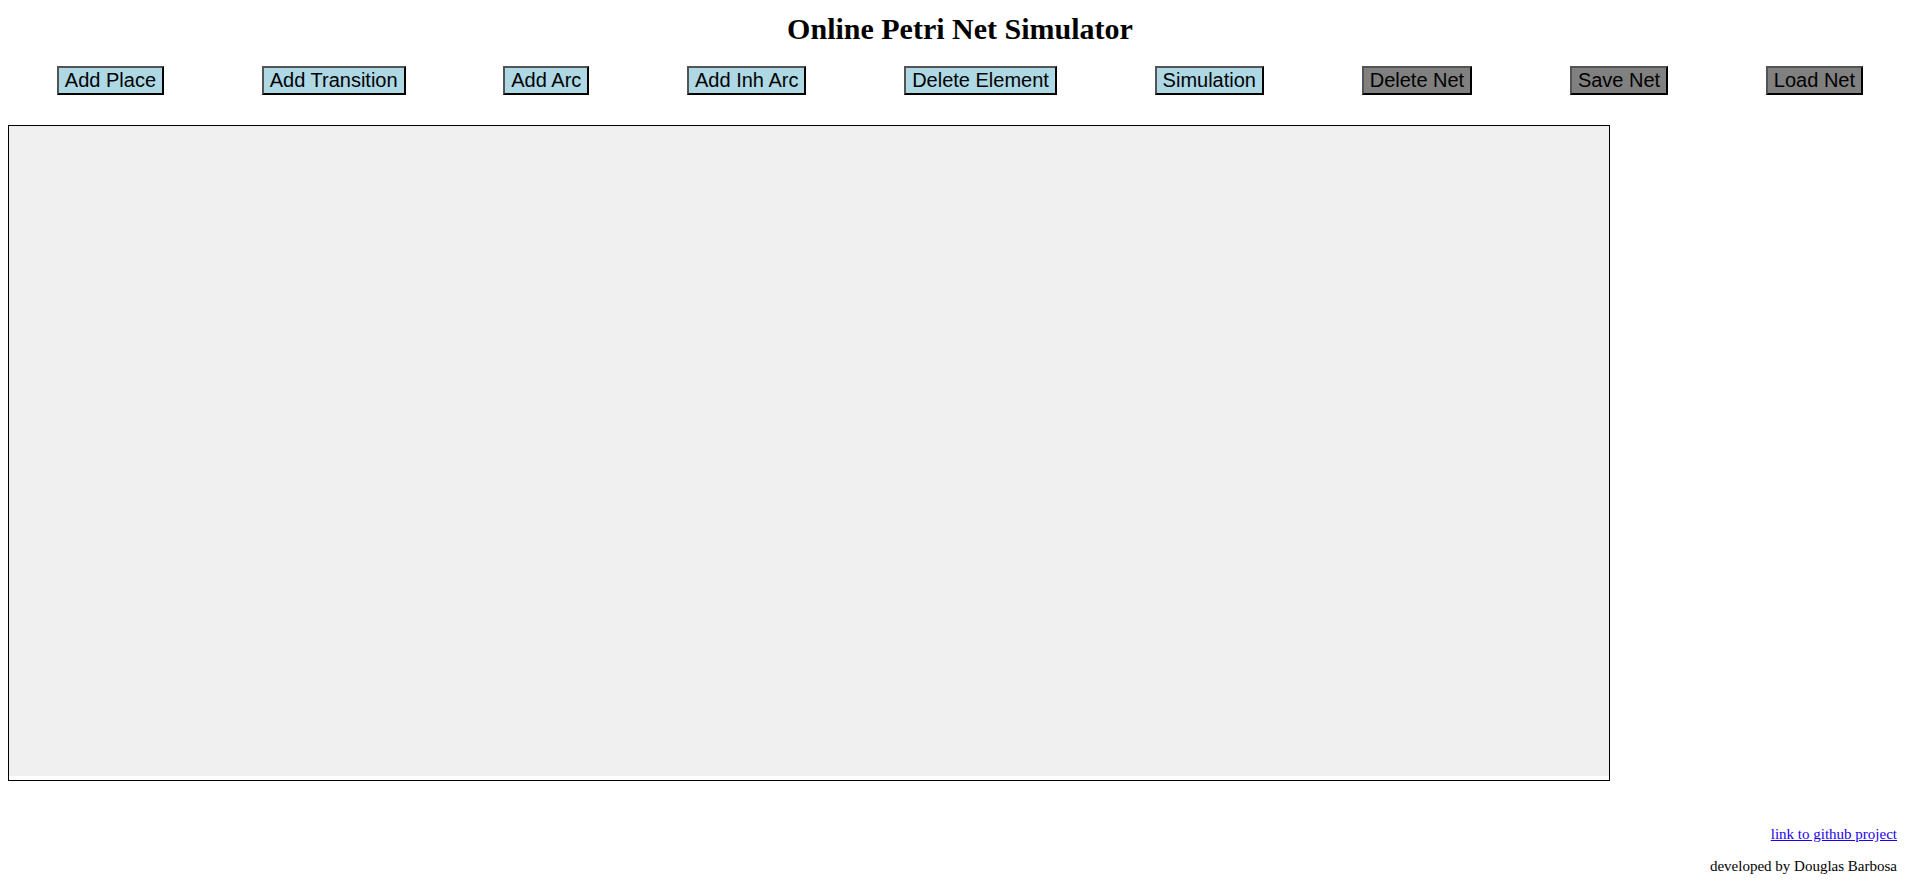
\includegraphics[scale=0.3]{figuras/area_canvas.png}
	\caption[Área canvas]{Retângulo da área \textbf{<canvas>} logo abaixo dos botões da aplicação web}
	\label{fig:area_canvas}
\end{figure}
\FloatBarrier

Tendo a área \textbf{canvas} definida, inicia-se a manipulação dos elementos gráficos que iram representar as redes de Petri. Para tornar possível a interatividade de diferentes elementos criou-se uma função de loop. Essa função tem como principal objetivo apagar e renderizar os elementos representados na área canvas de forma continua. Esse processo de apagar os elementos e renderizar novamente, várias vezes por segundo, permite criar animações, tornando possível a movimentação dos elementos e a edição das informações na tela. 

\lstinputlisting[caption={Função loop}, captionpos=b, label={lst:functionloop}]{scripts/functionLoop.js}

O método Javascript \textbf{\textit{window.requestAnimationFrame(loop, canvas)}} informa ao navegador que se deseja executar animações. Além disso, ele sincroniza a taxa de atualização, em \textbf{Hz}, das animações, com a taxa de atualização do monitor do usuário. Posteriormente, faz-se a chamada da função \textbf{\textit{render()}}, que irá renderizar os elementos na área \textbf{canvas}. Também, a função \textbf{\textit{buttonColors()}} é acionada. Ela verifica qual botão foi pressionado e, com base nas informações, altera a cor do botão que indica a ação a ser executada. 

Além, faz-se a verificação da variável \textbf{\textit{simulation}}, que indica ao código se está ocorrendo a ação de simulação da rede de Petri. Caso sim, a função \textbf{\textit{netSimulationEnables()}}, responsável pela simulação da rede de Petri \ref{cap:simulation}, é acionada.

\subsection*{Função de renderização}

A função \textbf{\textit{render()}} é responsável pela renderização de todos os elementos dentro da área \textbf{canvas} destinada a construção e simulação das redes de Petri. Ela utiliza a API do Javascript para a manipulação do \textbf{canvas}. Para cada tipo de elemento inicia-se o desenho com \textbf{\textit{beginPatch()}} e se finaliza com \textbf{\textit{beginPatch()}}

\begin{enumerate}
	\item renderização dos lugares;
	\item renderização das transições;
	\item renderização dos arcos;
	\item renderização dos pontos intermediário dos arcos;
	\item renderização do triângulo ou circulo na ponta do arco, a depender do tipo de arco;
	\item renderização do arco, enquanto ele é criado \ref{fig:mousemove_desenhando_arco};
	\item renderização do lugar após o botão \textbf{Add Place} ser pressionado, e antes de ser adicionado com \textbf{\textit{mousedown}};
	\item renderização da transição após o botão \textbf{Add Transition} ser pressionado, e antes de ser adicionado com \textbf{\textit{mousedown}}.
\end{enumerate}

\subsubsection*{Renderização dos lugares}

Um lugar é, graficamente, um circulo. Ao manipular o \textbf{canvas} é possível construir um circulo passando os seguintes parâmetros: as posições \textbf{x} e \textbf{y} do centro do circulo e o seu raio. 

\lstinputlisting[caption={Renderizando lugar}, captionpos=b, label={lst:renderPlace}]{scripts/renderPlace.js}

\begin{figure}[ht] 
	\centering
	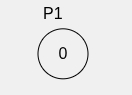
\includegraphics[scale=1]{figuras/renderPlace.png}
	\caption[renderPlace]{Lugar P1 renderizado na tela}
	\label{fig:renderPlace}
\end{figure}
\FloatBarrier

Além disso, um lugar possui algumas outras características, como o número de \textbf{\textit{tokens}} e o seu nome. Dessa forma, um número, representando a quantidade de \textbf{\textit{tokens}} é renderizado no centro do circulo. Um outro texto, representando o nome é renderizado um pouco acima do circulo, conforme \ref{lst:renderPlace}. A renderização ocorre de forma recursiva em cada um dos lugares que estão informados em \textbf{\textit{arrayPlaces}}.

\subsubsection*{Renderização das transições}

Uma transição é, graficamente, um retângulo. É possível construir um retângulo passando os seguintes parâmetros: posição \textbf{x} e \textbf{y} da ponta inferior esquerda do retângulo, largura e altura, em pixels. Além disso, a transição possui a cor preta quando a propriedade \textbf{\textit{isEnable}} é falsa. Quando \textbf{\textit{isEnable}} é verdadeiro, e a simulação está ativada, a cor da transição é vermelha. 

\lstinputlisting[caption={Renderizando transição}, captionpos=b, label={lst:renderTransition}]{scripts/renderTransition.js}

\begin{figure}[ht]
	\label{fig:renderTransition}
	\centering
	\begin{minipage}{0.5\textwidth}
		\centering
		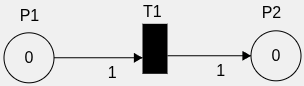
\includegraphics[scale=1]{figuras/transitionEnableFalse.png}
		%\caption[renderTransitionEnableFalse]{Transição renderizada não ativada}
		\label{fig:renderTransitionEnableFalse}
	\end{minipage}
	\hfill
	\begin{minipage}{0.5\textwidth}
		\centering
		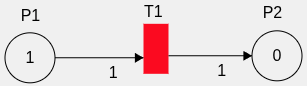
\includegraphics[scale=1]{figuras/transitionEnableTrue.png}
		%\caption[renderTransitionEnableTrue]{Transição renderizada ativada}
		\label{fig:renderTransitionEnableTrue}
	\end{minipage}
	\caption{Renderização da transição T1 de forma não ativada e ativada}
\end{figure}

Como o parâmetro a ser passado para a API do Javascript para a construção de um retângulo em uma área \textbf{canvas} exige as coordenadas \textbf{x} e \textbf{y} do canto inferior esquerdo do retângulo, fez-se uma compensação, utilizando os valores de altura e largura, para se obter a posição do centro do retângulo. Dessa forma, ao posicionar e movimentar uma transição, se faz pela posição do centro.  A renderização ocorre de forma recursiva em cada uma das transições que estão informados em \textbf{\textit{arrayTransitions}}.

\subsubsection*{Renderização dos arcos}

Um arco, graficamente, é uma linha. No caso específico das redes de Petri, temos 2 principais tipos de arcos, normal e inibidor. O arco normal é representado como uma seta, o arco inibidor é semelhante, mas possui um circulo na ponta, ao invés de um triângulo. O processo é feito recursivamente em cada um dos arcos contidos em \textbf{\textit{arrayArcs}}.

\lstinputlisting[caption={Renderizando arco}, captionpos=b, label={lst:renderArc}]{scripts/renderArc.js}

Inicialmente, para a renderização do arco, há uma detecção da posição \textbf{x} e \textbf{y}. Esse primeiro ponto precisar ser, necessariamente dentro de algum elemento, lugar ou transição para arcos normais, e, apenas lugar, para arcos inibidores. Tendo a primeira posição \textbf{x} e \textbf{y} definida, há duas opções: ou o usuário seleciona o elemento final do arco, ou ele seleciona um ponto intermediário. No primeiro caso, uma linha entre o ponto inicial e final é renderizada. Caso seja um arco normal, um triângulo na ponto é renderizado que, junto com a linha, dá a ilusão de ser uma seta direcional. No caso do arco inibidor, um circulo é renderizado na ponta final da linha. 

\begin{figure}[ht] 
	\centering
	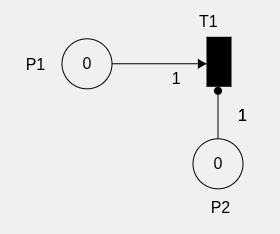
\includegraphics[scale=0.7]{figuras/arcNormalInibidor.png}
	\caption[Arco normal e inibidor]{Arco normal e inibidor chegando transição T1}
	\label{fig:arcNormalInibidor}
\end{figure}

Há também o segundo caso, em que o usuário cria um ponto intermediário. Nesse caso, uma linha entre o ponto inicial e o ponto intermediário é criada. Na posição \textbf{x} e y\textbf{y} desse ponto intermediário é criado um circulo, para indicar que ali tem um arco intermediário, e que pode ser movimentado posteriormente. Podem existir infinitos pontos intermediários, até que o usuário clique no elemento final, quando o desenho do arco finaliza. Na ponta final, há o triângulo ou circulo, a depender do tipo de arco. 

\begin{figure}[ht] 
	\centering
	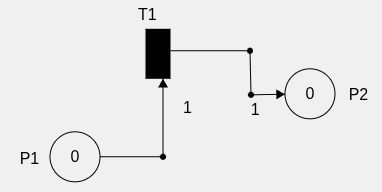
\includegraphics[scale=0.8]{figuras/arcPontoIntermediario.png}
	\caption[Arco com pontos intermediários]{Arcos com pontos intermediários}
	\label{fig:arcPontoIntermediario}
\end{figure}

Além disso, o arco é mostrado, em tempo real, enquanto é desenhado. Faz-se isso utilizando o ponto inicial, juntamente com os pontos intermediário, caso existam, e a posição final é a do ponteiro do mouse, obtida com \textbf{\textit{mousemove}} \ref{cap:mousemove}. O processo é o mesmo que o anterior, diferenciado-se pelo fato do ponto final ser o obtido pelas propriedades \textbf{\textit{clientX}} e \textbf{\textit{clientY}} do evento \textbf{\textit{mousemove}} \ref{fig:mousemove_desenhando_arco}. 

\section{Eventos do Javascript}

No desenvolvimento de aplicações web, é essencial que as páginas sejam responsivas e interativas. A linguagem Javascript nos fornece uma série de funcionalidades que permitem o desenvolvimento de eventos para a interatividade do usuário com as páginas que ele acessa. Os eventos representam ações e recorrências que ocorrem dentro do navegador do usuário, como cliques, movimentação do mouse, pressionamento de teclas no teclado, dentre outras ações que um usuário, normalmente, pode executar dentro de uma página na web. 

Para o desenvolvimento da aplicação web, capaz de construir e simular redes de Petri, é fundamental 3 principais eventos, sendo eles o \textbf{\textit{mousemove}}, \textbf{\textit{mousedown}} e \textbf{\textit{mouseup}}. Esses eventos permitem que o usuário consiga interagir com a área da página dedicada ao desenvolvimento das redes de Petri. 

\subsection*{mousemove}\label{cap:mousemove}

O evento \textbf{\textit{mousemove}} é disparado sempre que ocorre o movimento do ponteiro do mouse sobre um determinado elemento \cite{mdn_mousemove_event}. No caso da aplicação web desenvolvida, é acionado sempre que ocorre o movimento do ponteiro do mouse dentro da área delimitada para o desenvolvimento das redes de 

\lstinputlisting[caption={Exemplo da chamada do evento \textbf{\textit{mousemove}}}, captionpos=b, label={lst:eventmousemove}]{scripts/mousemove.js}

As propriedades \textbf{\textit{clientX}} e \textbf{\textit{clientY}} permitem definir a posição do ponteiro do mouse sempre que ele está se movendo. Utiliza-se desse evento, principalmente, para determinar se o cursor está sobre alguns dos elementos clicáveis na tela. Caso sim, ele altera o estilo do ponteiro. Quando está fora de algum elemento clicável, o ponteiro do mouse utiliza o estilo \textbf{\textit{default}}, e quando está sobre a área de algum elemento clicável, o estilo é alterado para \textbf{\textit{pointer}}.

\begin{figure}[ht] 
	\centering
	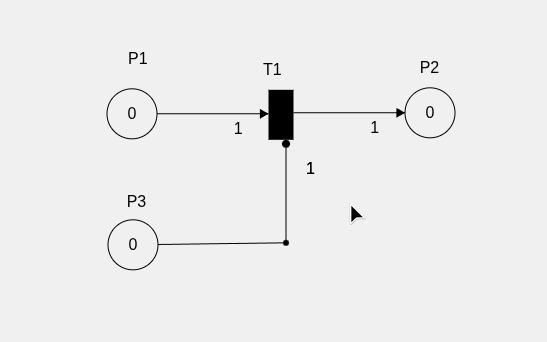
\includegraphics[scale=0.4]{figuras/mouse_estilo_default.png}
	\caption[Mouse estilo default]{Ponteiro do mouse com estilo \textbf{\textit{default}}}
	\label{fig:mouse_estilo_default}
\end{figure}

\begin{figure}[ht] 
	\centering
	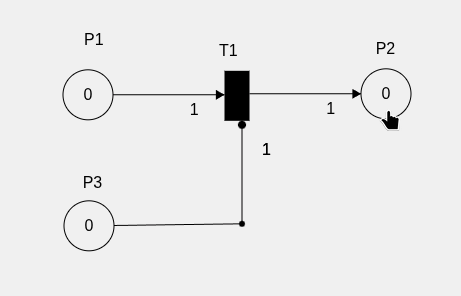
\includegraphics[scale=0.4]{figuras/mouse_estilo_pointer.png}
	\caption[Mouse estilo default]{Ponteiro do mouse com estilo \textbf{\textit{pointer}}}
	\label{fig:mouse_estilo_pointer}
\end{figure}

O evento \textbf{\textit{mousemove}} também é utilizado no momento de criação dos arcos, para renderizar o arco enquanto ele ainda está sendo desenhado. Por exemplo, ao clicar no primeiro elemento, lugar ou transição, onde o arco iniciará, uma posição inicial é detectada. Após, espera-se que o usuário clique, ou num ponto intermediário do arco, ou no ponto final do arco. Enquanto o ponto final, no segundo elemento, não é detectado, utiliza-se da posição do ponteiro do mouse, nos eixos \textbf{x} e \textbf{y}, do evento \textbf{\textit{mousemove}} para renderizar uma linha entre a última posição fixa detectada e a posição do ponteiro do mouse.

\begin{figure}[ht] 
	\centering
	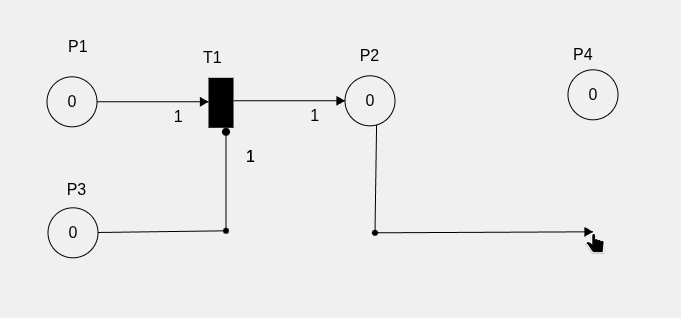
\includegraphics[scale=0.4]{figuras/mousemove_desenhando_arco.png}
	\caption[Mousemove desenhando arco]{Arco sendo renderizado antes de ser concluído com \textbf{\textit{mousemove}}}
	\label{fig:mousemove_desenhando_arco}
\end{figure}

\subsection*{mousedown}\label{cap:mousedown}

O evento \textbf{\textit{mousedown}} é disparado sempre que ocorre o pressionamento de um botão do mouse sobre um determinado elemento \cite{mdn_mousedown_event}. No caso da aplicação web desenvolvida, é acionado sempre que ocorre o clique do mouse dentro da área delimitada para o desenvolvimento das redes de Petri. 

\lstinputlisting[caption={Exemplo da chamada do evento \textbf{\textit{mousedown}}}, captionpos=b, label={lst:eventmousedown}]{scripts/mousedown.js}

Através do evento \textbf{\textit{mousedown}} é possível determinar a posição \textbf{x} e \textbf{y} em que ocorreu um clique. Com isso, verifica-se qual dos botões de ação está pressionado. Por exemplo, caso o botão \textbf{Add Place} esteja ativado, um lugar, na posição \textbf{x} e \textbf{y}, onde ocorreu o clique, será adicionado. O mesmo vale para transições e arcos. Além disso, é possível determinar se o clique ocorreu dentro de algum elemento. Isso é essencial para determinar o elemento inicial e final de um arco. 

Em combinação com o evento \textbf{\textit{mouseup}} \ref{cap:mouseup} define-se, também, se algum botão do mouse está sendo pressionado continuamente, ou seja, se o usuário clicou e segurou o botão pressionado. 

\subsection*{mouseup}\label{cap:mouseup}

O evento \textbf{\textit{mouseup}} é disparado sempre que ocorre a soltura de um botão do mouse após ele ter sido pressionado \cite{mdn_mouseup_event}. No caso da aplicação web desenvolvida, é acionado sempre que ocorre a soltura do botão após ele ter sido pressionado dentro da área delimitada para o desenvolvimento das redes de Petri.

\lstinputlisting[caption={Exemplo da chamada do evento \textbf{\textit{mouseup}}}, captionpos=b, label={lst:eventmouseup}]{scripts/mouseup.js}

O evento \textbf{\textit{mouseup}} é utilizado, principalmente, em conjunto com o evento \textbf{\textit{mousedown}} \ref{cap:mousedown}. Essa junção permite saber quando um botão do mouse está sendo continuamente pressionado. Com essa funcionalidade, podemos executar ações de movimentação dos nossos elementos \ref{cap:move_elements}, como lugares, transições, nome de elementos, dentre outros. 

\lstinputlisting[caption={Lógica para botão continuamente pressionado \textbf{\textit{isPress}}}, captionpos=b, label={lst:ispress}]{scripts/isPress.js}

Quando ocorre o evento \textbf{\textit{mousedown}}, a variável \textbf{\textit{isPress}} recebe o valor verdadeiro. Enquanto o evento \textbf{\textit{mouseup}} não ocorre, a variável permanece como verdadeiro, indicando para o código que o botão está sendo pressionado. Além disso, quando \textbf{\textit{isPress}} é verdadeiro, e ele está sobre algum dos elementos, o estilo do cursor muda para \textbf{\textit{grabbing}}, um estilo que mostra para o usuário que aquele elemento pode ser movimentado. 

\begin{figure}[ht] 
	\centering
	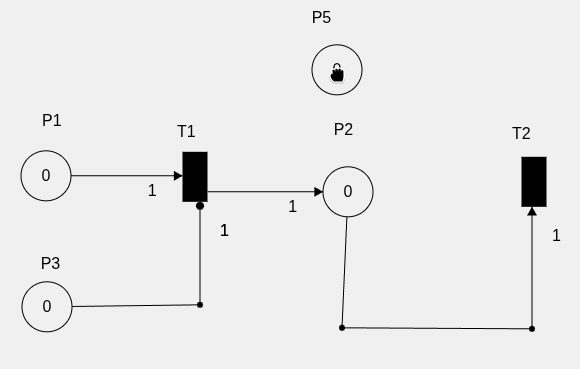
\includegraphics[scale=0.4]{figuras/mouse_estilo_grabbing.png}
	\caption[Mouse estilo grabbing]{Ponteiro do mouse com estilo \textbf{\textit{grabbing}}}
	\label{fig:mouse_estilo_grabbing}
\end{figure}

\section{Criação dos elementos}


\subsection*{Criação dos lugares}

Para a criação dos lugares foi criado um primeiro botão através do arquivo \textit{\textbf{index.html}}. No momento em que se pressiona o botão \textit{\textbf{AddPlace}} a função \textit{\textbf{buttonAddPlace}} é chamada e seu script é executado. Nessa função, a variável global \textit{\textbf{buttonPress}} sofre a alteração de seu valor, caso seu valor seja diferente de \textit{\textbf{1}}, o valor \textit{\textbf{1}} é atribuído, do contrário seu valor retorna para zero.

\lstinputlisting[caption={Função buttonAddPlace}, captionpos=b, label={lst:buttonAddPlace}]{scripts/buttonAddPlace.js}

Quando \textit{\textbf{buttonPress = 1}} espera-se que o usuário clique na área demarcada para a construção de sua rede de Petri. No momento do clique, o evento \textit{\textbf{mousedown}} é detectado e seu script é executado. No script do evento \textit{\textbf{mousedown}} se faz uma verificação do valor da variável \textit{\textbf{buttonPress}}. Como o valor atribuído é \textit{\textbf{1}} se faz uma chamada da função \textit{\textbf{addPlace}} passando-se os valores \textbf{\textit{mouseX}} e \textbf{\textit{mouseY}}. 

\lstinputlisting[caption={Chamada da função addPlace}, captionpos=b, label={lst:chamadaAddPlace}]{scripts/chamadaAddPlace.js}

Na função \textbf{\textit{addPlace}} se constroi um objeto \textbf{\textit{(objPlace)}} com as seguintes propriedades: 

\begin{enumerate}
	\item \textbf{id:} representa a identidade única que irá identificar esse objeto ao longo de todo o código;
	\item \textbf{name:} semelhante ao id, mas editável pelo usuário. Esse é o valor mostrado na tela quando se cria o objeto lugar;
	\item \textbf{namePositionX:} indica o valor do eixo X em que o \textbf{\textit{name}} do objeto se encontra na tela;
	\item \textbf{namePositionY:} indica o valor do eixo Y em que o \textbf{\textit{name}} do objeto se encontra na tela;
	\item \textbf{posX:} indica o valor do eixo X em que o objeto se encontra na tela;
	\item \textbf{posY:} indica o valor do eixo X em que o objeto se encontra na tela;
	\item \textbf{connections:} array que identifica quais outros objetos estão ligados a ele;\label{prop:connections}
	\item \textbf{nTokens:} identifica quantos \textbf{\textit{tokens}} o objeto lugar possuí.
\end{enumerate}

Após a definição desses valores no \textbf{\textit{objPlace}} se faz a inserção do mesmo no \textbf{\textit{arrayPlaces}}, em que se encontra todos os outros objetos de mesmas propriedades. Também se faz o acréscimo de \textbf{\textit{1}} na contagem de quantos lugares existem até o momento.

\lstinputlisting[caption={Função addPlace}, captionpos=b, label={lst:functionAddPlace}]{scripts/addPlace.js}

Posteriormente a execução da função \textbf{\textit{addPlace}}, o valor da variável \textbf{\textit{buttonPress}} é atribuído como \textbf{\textit{0.}}

\newpage

\begin{figure}[h!]
	\centering
	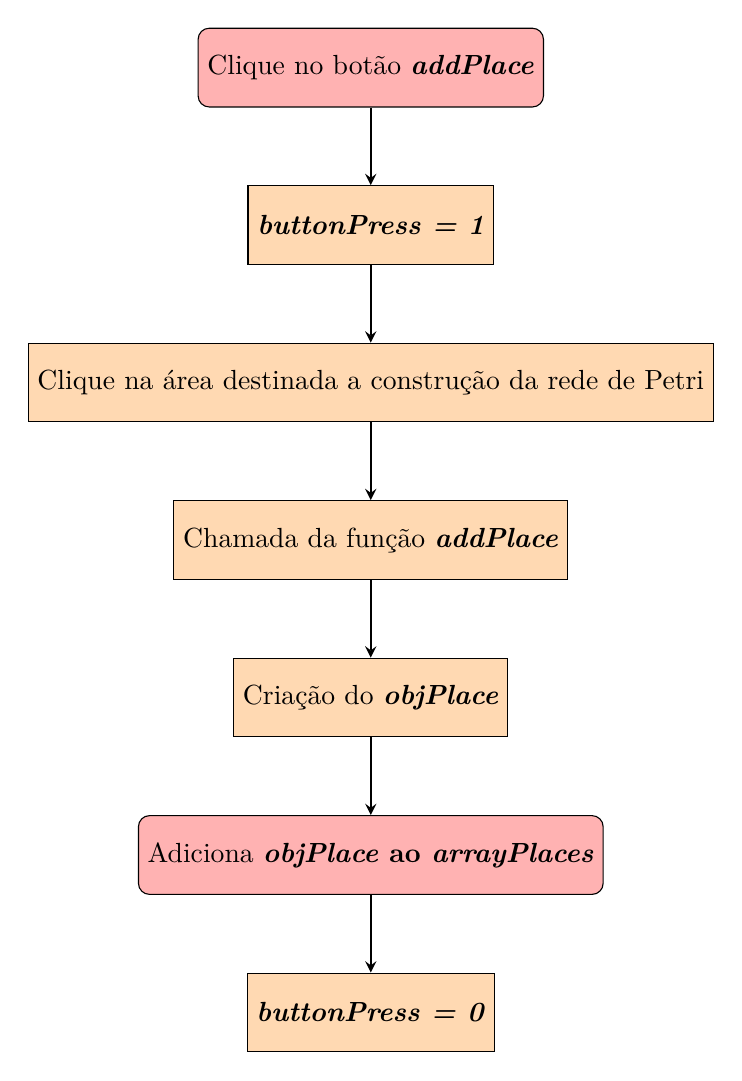
\begin{tikzpicture}[node distance=2cm]
		
		% Nodes
		\node (start) [startstop] {Clique no botão \textbf{\textit{addPlace}}};
		\node (step) [process, below of=start] {\textbf{\textit{buttonPress = 1}}};
		\node (step1) [process, below of=step] {Clique na área destinada a construção da rede de Petri};
		\node (step2) [process, below of=step1] {Chamada da função \textbf{\textit{addPlace}}};
		\node (step3) [process, below of=step2] {Criação do \textbf{\textit{objPlace}}};
		\node (end) [startstop, below of=step3] {Adiciona \textbf{\textit{objPlace} ao \textbf{\textit{arrayPlaces}}}};
		\node (step4) [process, below of=end] {\textbf{\textit{buttonPress = 0}}};
		
		% Arrows
		\draw [arrow] (start) -- (step);
		\draw [arrow] (step) -- (step1);
		\draw [arrow] (step1) -- (step2);
		\draw [arrow] (step2) -- (step3);
		\draw [arrow] (step3) -- (end);
		\draw [arrow] (end) -- (step4);
		
	\end{tikzpicture}
	\caption{Diagrama de fluxo para adicionar um lugar}
	\label{fig:fluxo4etapas}
\end{figure}

\newpage

Para facilitar a visualização no momento da adição do lugar, um efeito sombreado, representando o lugar, é mostrado enquanto se movimenta o mouse, antes do clique na tela, na área destinada a construção da rede de Petri, conforme a imagem abaixo:

\begin{figure}[ht] 
	\centering
	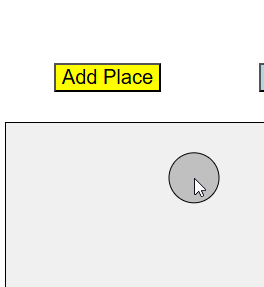
\includegraphics[scale=0.55]{figuras/exemplo_clique_addPlace.png}
	\caption[Clicando bo botao addPlace]{Clique no botão addPlace}
	\label{fig:clique_add_place}
\end{figure}

\subsection*{Criação das transições}

De modo semelhante a criação de lugares, temos um segundo botão, criado através do arquivo \textbf{\textit{index.html}}, denominada \textbf{\textit{Add Transition}}. Seu modo de funcionamento é análogo ao botão \textbf{\textit{Add Place}}. No momento de seu clique, a função \textbf{\textit{buttonAddTransition()}} é chamada. Suas orientãções também alterarm o valor da variável global \textbf{\textit{buttonPress}}. Quando seu valor é diferente de \textbf{\textit{2}}, o valor \textbf{\textit{2}} é atribuído, caso contrário o valor retorna para zero. 

\lstinputlisting[caption={Função buttonAddTransition}, captionpos=b, label={lst:buttonAddTransition}]{scripts/buttonAddTransition.js}

No momento do clique do botão \textbf{\textit{Add Transition}} espera-se que o usuário faça um clique na área destinada a construção da rede de Petri. Dessa forma, fazendo o clique, uma transição é adicionada na mesma posição em que ocorreu o clique. Nesse momento, o evento \textbf{\textit{mousedown}} é chamado e se faz uma verifição do valor da variável \textbf{\textit{buttonPress}}. Como o valor é igual a \textbf{\textit{2}}, a função \textbf{addTransition()} é chamada, passando-se os valores \textbf{\textit{mouseX}} e \textbf{\textit{mouseY}}.

\lstinputlisting[caption={Chamada da função addTransition()}, captionpos=b, label={lst:chamadaAddTransition}]{scripts/chamadaAddTransition.js}

Na função \textbf{addTransition()} se constrói um objeto \textbf{\textit{objTransition}} com as seguintes propriedades:

\begin{enumerate}
	\item \textbf{id:} representa a identidade única da transição que irá identificar esse objeto ao longo de todo o código;
	\item \textbf{name:} semelhante ao id, mas editável pelo usuário. Esse é o valor mostrado na tela quando se cria o objeto trasição;
	\item \textbf{namePositionX:} indica o valor do eixo X em que o \textbf{\textit{name}} da transição se encontra na tela;
	\item \textbf{namePositionY:} indica o valor do eixo Y em que o \textbf{\textit{name}} da transição se encontra na tela;
	\item \textbf{posX:} indica o valor do eixo X em que a transição se encontra na tela;
	\item \textbf{posY:} indica o valor do eixo Y em que a transição se encontra na tela;
	\item \textbf{connections:} array que identifica quais outros objetos estão ligados a essa transição;
	\item \textbf{isEnable:} valor booleano que indica se as exigências para ativação da transição foram cumpridas.\label{prop:isEnable}
\end{enumerate}

Após as definições desses valores no \textbf{\textit{objTransition}} se faz a inserção do mesmo no \textbf{\textit{arrayTransitions}}, em que se encontra todas as outras transições de mesmas propriedades. Também se faz o acréscimo de \textbf{\textit{1}} na contagem de quantas transições existem até o momento.

\lstinputlisting[caption={Função addTransition()}, captionpos=b, label={lst:addTransition}]{scripts/addTransition.js}

Posteriormente a execução da função \textbf{\textit{addTransition()}}, o valor da variável \textbf{\textit{buttonPress}} é atribuído como \textbf{\textit{0}}

Para facilitar a visualização no momento de adição da transição, o botão pressionado permanece na cor amarela enquanto o clique na tela não ocorre para adição da transição. Além disso, um efeito sombreado, em forma de uma transição acompanha o cursor do mouse enquanto não há o clique, conforme imagem abaixo: 

\begin{figure}[ht] 
	\centering
	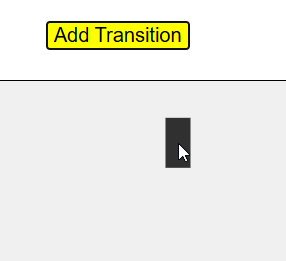
\includegraphics[scale=0.55]{figuras/exemplo_clique_addTransition.png}
	\caption[Clicando bo botao addTransition]{Clique no botão Add Transition}
	\label{fig:clique_add_transition}
\end{figure}


\newpage

\begin{figure}[h!]
	\centering
	\begin{tikzpicture}[node distance=2cm]
		
		% Nodes
		\node (start) [startstop] {Clique no botão \textbf{\textit{Add Transition}}};
		\node (step1) [process, below of=start] {\textbf{\textit{buttonPress = 2}}};
		\node (step2) [process, below of=step1] {Clique na área destinada a construção da rede de Petri};
		\node (step3) [process, below of=step2] {Chamada da função \textbf{\textit{addTransition}}};
		\node (step4) [process, below of=step3] {Criação do \textbf{\textit{objTransition}}};
		\node (step5) [process, below of=step4] {Adiciona \textbf{\textit{objTransition} ao \textbf{\textit{arrayTransitions}}}};
		\node (step6) [process, below of=step5] {A transição é renderizada na tela na posição \textbf{\textit{mouseX}} e \textbf{\textit{mouseY}}};
		\node (end) [startstop, below of=step6] {\textbf{\textit{buttonPress = 0}}};
		
		% Arrows
		\draw [arrow] (start) -- (step);
		\draw [arrow] (step1) -- (step2);
		\draw [arrow] (step2) -- (step3);
		\draw [arrow] (step3) -- (step4);
		\draw [arrow] (step4) -- (step5);
		\draw [arrow] (step5) -- (step6);
		\draw [arrow] (step6) -- (end);
		
	\end{tikzpicture}
	\caption{Diagrama de fluxo para adicionar uma transição}
	\label{fig:fluxo_add_transition}
\end{figure}

\newpage

\subsection*{Criação dos arcos}

Para a criação dos arcos foram desenvolvido dois novos botões, denominados \textbf{\textit{Add Arc}}, para a criação de arcos normais, e \textbf{\textit{Add Inh Arc}}, para a criação de arcos inibidores. No momento do clique, eles desempenham funções semelhantes, diferenciando-se apenas pela valor da variável \textit{\textbf{buttonPress}} e \textbf{\textit{arcType}}. O papel dessas variáveis é indicar o botão que foi pressionado e o tipo de arco selecionado. Além disso, a variável booleana  \textbf{\textit{drawArc}} recebe o valor \textbf{\textit{true}} indicando que um arco será desenhado na tela.

\lstinputlisting[caption={Botão Add Arc}, captionpos=b, label={lst:buttonAddArc}]{scripts/buttonAddArc.js}

\lstinputlisting[caption={Botão Add Inh Arc}, captionpos=b, label={lst:buttonAddInhArc}]{scripts/buttonAddInhArc.js}

No momento de acionamento de algum desses dois botões espera-se que o usuário inicie o desenho de um arco. Para isso, inicialmente ele deve selecionar o ponto inicial do desenho desse arco. Para arcos normais, o ponto inicial pode ser tanto um lugar, quanto por uma transição. Para os arcos inibidores, o ponto inicial deve ser obrigatoriamente um lugar, não é possível iniciar o desenho de um arco inibidor a partir de uma transição. Quando o usuário faz o primeiro clique, posterior ao clique do botão, o evento \textbf{\textit{mousedown}} é ativado e a verificação da variável \textbf{\textit{buttonPress}} é verificado. Caso \textbf{\textit{buttonPress}} seja igual a \textbf{\textit{3}} ou \textbf{\textit{4}} a função \textbf{\textit{addArc}} é chamada. Como o valor da variável \textbf{\textit{buttonPress}} não se altera ao longo do desenho do arco, sempre que há um clique na tela, há a chamada da função \textbf{\textit{addArc}}.

A cada chamada da função \textbf{\textit{addArc}} se faz uma verificação de algumas variáveis temporárias que auxiliam a construção dos arcos, são elas: 

\begin{enumerate}
	\item \textbf{\textit{startingPositionArc:}} array que indica o ponto inicial, nos eixos X e Y da tela, do arco, além de contter o id do item em que o arco se inicia;
	\item \textbf{\textit{intermediatePoints:}} array que indica todos os pontos, nos eixos X e Y da tela, depois do ponto inicial e antes do ponto final;
	\item \textbf{\textit{endPositionArc:}} array que indica a ponto final, nos eixos X e Y da tela, do arco, além de contter o id do item em que o arco termina.
\end{enumerate}

A primeira verificação que se faz na função \textbf{\textit{addArc}} é a existência de pontos intermediários. Para essa vericação analisamos o tamanho do array \textbf{\textit{startingPositionArc}} e \textbf{\textit{endPositionArc}}. Se o primeiro for maior que \textbf{\textit{0}}, e o último igual a \textit{\textbf{0}}, significa que o clique foi feito para a construção de um ponto intermediário  arco. Dessa forma, se faz uma inserção no array \textbf{\textit{intermediatePoints}} da posição dos eixos X e Y, passando-se os valores das variáveis \textbf{\textit{mouseX}} e \textbf{\textit{mouseY}}.

\lstinputlisting[caption={Verificação de pontos intermediários}, captionpos=b, label={lst:intermediatePoints}]{scripts/intermediatePoints.js}

Caso a condição anterior não seja atendida, se entende que o ponto \textbf{\textit{X}} e \textbf{\textit{Y}} não representa um ponto intermediário do arco. Posteriormente, se percorre os arrays \textbf{\textit{arrayPlaces}} e \textbf{\textit{arrayTransition}}. Para cada uma das posições de ambos os arrays se faz a verificação, através das funções \textbf{\textit{isInsidePlace}} e \textbf{\textit{isInsideTransition}}, se o clique do mouse ocorreu dentro de algum dos lugares ou transições que estão dispostas na tela. Caso o clique ocorra dentro de algum desses dois elementos, o ponto \textbf{\textit{X}} e \textbf{\textit{Y}} será gravado na variável \textbf{\textit{startingPositionArc}}, juntamente com o \textbf{\textit{id}} do elemento em que o arco se iniciou. 

\subsection*{Para lugares}

Caso a chamada da função \textbf{\textit{isInsidePlace}} retorne \textbf{\textit{true}} e a variável \textbf{\textit{startingPositionArc}} não contenha nenhum valor, o ponto inicial, com os eixos \textbf{\textit{X}} e \textbf{\textit{Y}} e o id do lugar, são gravados nas propriedades do arco. Além disso, no lugar em quem o arco se iniciou, insere-se a informação de que aquele arco se iniciou ali. A variável auxiliar \textbf{\textit{typeElement}} também recebe o valor \textbf{\textit{"place"}}, para indicar que aquele arco se iniciou num lugar. 

Caso a verificação anterior não seja atendida, se faz uma nova verificação. Se a chamada da função \textbf{\textit{isInsidePlace}} retornar \textbf{\textit{true}} e a variável \textbf{\textit{typeElement}} contiver o valor \textbf{\textit{"transition"}}, quer dizer que o arco se iniciou em uma transição, e agora está finalizando em um lugar. Com isso, se adiciona o valor \textbf{\textit{X} e \textbf{\textit{Y}}} do clique e o \textbf{\textit{id}} do lugar em que o arco está finalizando na variável \textbf{\textit{endPositionArc}} que, posteriormente, será adicionado nas propriedades do arco. O lugar recebe a informação de que esse arco finalizou nele.

Com a finalização do arco, a variável \textbf{\textit{drawArc}} recebe o valor \textbf{\textit{false}} e a \textbf{\textit{typeElement}} recebe \textbf{\textit{null}}

\lstinputlisting[caption={Construção de arco verificando os lugares}, captionpos=b, label={lst:arcPlace}]{scripts/arcPlace.js}

\subsection*{Para transições}

Caso a chamada da função \textbf{\textit{isInsideTransition}} retorne \textbf{\textit{true}} e a variável \textbf{\textit{startingPositionArc}} não contenha nenhum valor, o ponto inicial, com os eixos \textbf{\textit{X}} e \textbf{\textit{Y}} e o id da transição, são gravados nas propriedades do arco. Além disso, na transição em quem o arco se iniciou, insere-se a informação de que aquele arco se iniciou ali. A variável auxiliar \textbf{\textit{typeElement}} também recebe o valor \textbf{\textit{"transition"}}, para indicar que aquele arco se iniciou numa transição. 

Caso a verificação anterior não seja atendida, se faz uma nova verificação. Se a chamada da função \textbf{\textit{isInsideTransition}} retornar \textbf{\textit{true}} e a variável \textbf{\textit{typeElement}} contiver o valor \textbf{\textit{"place"}}, quer dizer que o arco se iniciou em um lugar, e agora está finalizando em uma transição. Com isso, se adiciona o valor \textbf{\textit{X} e \textbf{\textit{Y}}} do clique e o \textbf{\textit{id}} da transição em que o arco está finalizando na variável \textbf{\textit{endPositionArc}} que, posteriormente, será adicionado nas propriedades do arco. A transição recebe a informação de que esse arco finalizou nele.

Com a finalização do arco, a variável \textbf{\textit{drawArc}} recebe o valor \textbf{\textit{false}} e a \textbf{\textit{typeElement}} recebe \textbf{\textit{null}}

\lstinputlisting[caption={Construção de arco verificando as transições}, captionpos=b, label={lst:arcTransition}]{scripts/arcTransition.js}

\subsection*{Criando o arco com as propriedades}

Quando as variáveis temporárias \textbf{\textit{startingPositionArc}} e \textbf{\textit{endPositionArc}} apresentam valores atribuídos significa que todas as propriedades para se construir um arco estão satisfeitas, são elas:

\begin{enumerate}
	\item \textbf{id:} representa a identidade única do arco que irá identificar esse objeto ao longo de todo o código;
	\item \textbf{name:} identificador visual e textual do arco na tela;
	\item \textbf{type:} indica o tipo do arco, se ele é do tipo normal ou inibidor;
	\item \textbf{startingPositionArc:} indica o valor dos eixos X e Y em que o arco se inicia;
	\item \textbf{endPositionArc:} indica o valor dos eixos X e Y em que o arco finaliza;
	\item \textbf{start:} indica o id do elemento em que o arco se inicia;
	\item \textbf{end:} indica o id do elemento em que o arco finaliza;
	\item \textbf{intermediatePoints:} cada posição representa o valor dos eixos X e Y de um ponto intermediário do arco;
	\item \textbf{isEnable:} valor booleano que indica se as exigências para ativação daquele arco estão satisfeitas.
	\item \textbf{weight:} indica o peso do arco.
	\item \textbf{weightPos:} indica o valor dos eixos X e Y em que o peso do arco será mostrado na tela.
\end{enumerate}

Tendo essas propriedades definidas se faz a adição do arco no \textbf{\textit{arrayArcs}}. Por fim, as variáveis temporárias são atribuídas com valores nulos para que o próximo arco possa ser construído.

\lstinputlisting[caption={Criando o arco com as propriedades}, captionpos=b, label={lst:addArc}]{scripts/addArc.js}

\section{Movimentando elementos na tela}\label{cap:move_elements}

A movimentação de elementos é essencial para a construção de uma rede de Petri. A partir do momento em que os elementos são dispostos na tela, eles necessitam ser movimentados para uma melhor visualização e compreensão da rede. Os elementos, por vezes, podem ficar sobrepostos e mal distribuídos no momento de sua criação, gerando desconforto visual. Os elementos que podem ser movidos são: 

\begin{enumerate}
	\item lugares;
	\item transições;
	\item nome dos elementos;
	\item pontos intermediários dos arcos.
\end{enumerate}

Outros elementos, como número de \textbf{\textit{tokens}}, peso dos arcos, além dos pontos \textbf{x} e \textbf{y}, iniciais e finais dos arcos, acompanham a movimentação dos elementos principais, que podem ser movidos. Ou seja, não é possível movê-los diretamente.

\begin{figure}[ht]
	\centering
	\begin{minipage}{0.49\textwidth}
		\centering
		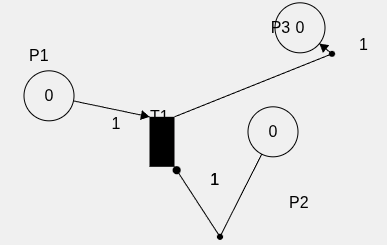
\includegraphics[scale=0.5]{figuras/move_mal_distribuido.png}
		%\caption[move_mal_distribuido]{move_mal_distribuido}
		\label{fig:move_mal_distribuido}
	\end{minipage}
	\hfill
	\begin{minipage}{0.49\textwidth}
		\centering
		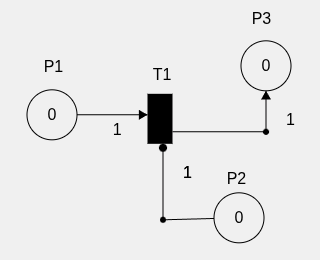
\includegraphics[scale=0.5]{figuras/move_bem_distribuido.png}
		%\caption[move_bem_distribuido]{\textbf{move_bem_distribuido}}
		\label{fig:move_mal_distribuido}
	\end{minipage}
	\caption{Elementos mal distribuídos e movimentados para uma melhor visualização.}
\end{figure}
\FloatBarrier


Além disso, alguns critérios precisam ser atendidos para que o movimento do elemento ocorra. É necessário que o cursor do mouse seja pressionado e segurado dentro da área do elemento a ser movimentado. Para isso, se torna fundamental descobrir se um clique ocorreu dentro da área dos elementos que podem se movimentar. No caso dos lugares e pontos intermediários, se calcula se o clique ocorreu dentro da área do circulo que os formam. No caso das transições e nome dos elementos, se calcula com base no retângulo que os formam. 

\subsection*{Verificando clique em círculos}

Ao clicarmos na área \textbf{canvas} obtemos o ponto \textbf{x} e \textbf{y} onde ele ocorreu. Assim, temos 2 possibilidades: ocorreu dentro do circulo, no caso, lugar ou ponto intermediário, ou fora. Para determinar se o clique ocorreu dentro de algum dos circulos distribuidos na área \textbf{canvas} calcula-se o comprimento entre o ponto \textbf{x} e \textbf{y} do clique e o ponto \textbf{x} e \textbf{y} central de cada circulo \cite{Macoratti2014}, de forma recursiva. Caso esse comprimento seja inferior ou igual ao raio de algum desses circulos, podemos afirmar que ele ocorreu dentro de algum elemento. Caso contrário, ocorreu fora.

O cálculo é feito utilizando-se da fórmula para distância entre 2 pontos. 

\begin{equation}\label{eq:distancia_entre_pontos}
	d_{AB}^2 = (x_B - x_A)^2 + (y_B - y_A)^2
\end{equation}


\lstinputlisting[caption={Verificando clique e atualizando posição do circulo}, captionpos=b, label={lst:insidePlace}]{scripts/insidePlace.js}

Tendo o retorno da função e a variável \textbf{\textit{isPress}} \ref{lst:ispress} como verdadeiro, há a satisfação das condições necessárias para movimentar o elemento. Dessa forma, a nova posição do centro do circulo é a posição do ponteiro do mouse, obtida com \textbf{\textit{mousemove}} \ref{cap:mousemove}. A movimentação ocorrerá até que o botão do mouse deixe de ser pressionado. 

\subsection*{Verificando clique em retângulos}

As transições e nome de elementos podem ser caracterizados como retângulos dentro da área \textbf{canvas}. Ao clicar na área \textbf{canvas} obtemos as posições \textbf{x} e \textbf{y} do clique. Para determinarmos se o clique ocorreu dentro de algum dos retângulos verifica-se e comparara-se o ponto \textbf{x} e \textbf{y} do clique com o ponto inferior esquerdo do retângulo \cite{Manzoni2013}. Faz-se a verificação da seguinte forma:

\begin{enumerate}
	\item $mouseX \geq transitionX$;
	\item $mouseX \leq transitionX + transitionWidth$;
	\item $mouseY \geq transitionY$;
	\item $mouseY \leq transitionY + transitionHeigth$.
\end{enumerate}

\begin{figure}[h!]
	\centering
	\begin{tikzpicture}[scale=1]
		% Eixos
		\draw[->] (-1,0) -- (6,0) node[right] {$x$};
		\draw[->] (0,-1) -- (0,5) node[above] {$y$};
		
		% Pontos do retângulo
		\coordinate (A) at (2,1);
		\coordinate (B) at (4,1);
		\coordinate (C) at (4,4);
		\coordinate (D) at (2,4);
		
		
		% Retângulo
		\draw[thick, black] (A) -- (B) -- (C) -- (D) -- cycle;
		
		% Nomeando os pontos
		\fill (A) circle (2pt) node[below left] {\scriptsize $transitionX, transitionY$};
		\fill (B) circle (2pt) node[below right] {\scriptsize $transitionX + transitionWidth$};
		\fill (C) circle (2pt) node[above right] {$$};
		\fill (D) circle (2pt) node[above left] {\scriptsize $transitionY + transitionHeigth$};
		
	\end{tikzpicture}
	\caption{Transição representada no plano cartesiano.}
\end{figure}


\lstinputlisting[caption={Verificando clique e atualizando posição do retângulo}, captionpos=b, label={lst:insideTransition}]{scripts/insideTransition.js}

Caso todas essas comparações sejam verdadeiras, pode-se concluir que o clique ocorreu dentro de algum retângulo. Com isso, tendo \textbf{\textit{isPress}} verdadeira, move-se o retângulo. A posição central do retângulo será a mesma do ponteiro do mouse. 

\section{Exclusão}

A partir do momento em que elementos são criados, há a necessidade de poder excluí-los, seja para corrigir algum erro, testar novas possibilidades, ou seja para deletar tudo e iniciar de novo. Na aplicação web desenvolvida buscou-se focar na exclusão tanto dos elementos individualmente, no caso, lugares, transições e arcos, quanto também pela exclusão da rede por completo, excluindo tudo de uma única vez.

{\color{red}criar fluxo para explicar o processo}


\begin{figure}[ht] 
	\centering
	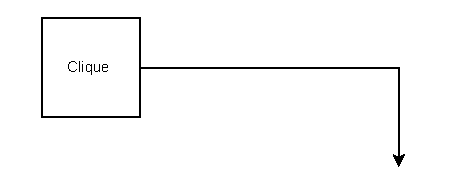
\includegraphics[scale=1]{figuras/deleteDiagram.pdf}
	\caption[Fluxograma Delete Elements]{Diagrama de fluxo para exclusão}
	\label{fig:deleteDiagram}
\end{figure}
\FloatBarrier

\subsection*{Deletando elementos}

Para deletar um elemento, de forma individual, é necessário clicar no botão \textbf{\textit{Delete Element}}. A partir dessa ação há 3 possibilidades: 

\begin{enumerate}
	\item exclusão de um lugar;
	\item exclusão de uma transição;
	\item exclusão de um arco.
\end{enumerate}

Para deletar um lugar, ou transição, o processo é semelhante. Além de deletar o elemento em si, há a necessidade de deletar os arcos que chegam e que saem, visto que, os arcos são dependentes desses elementos. Após o clique no botão \textbf{\textit{Delete Element}} há a mudança do valor da variável \textbf{\textit{buttonPress}} para \textbf{5} e, em seguida, quando ocorrer o evento \textbf{\textit{mousedown}} \ref{cap:mousedown}, há a chamada da função \textbf{\textit{deleteElements()}}. 

A função percorre os 3 arrays principais de elementos, \textbf{\textit{arrayPlaces}}, \textbf{\textit{arrayTransitions}} e \textbf{\textit{arrayArcs}}. Dessa forma, há a verificação da ocorrência de um clique dentro da área de algum dos elementos que podem ser excluídos: lugar, transição ou arco. No caso dos arcos, verifica-se se o clique ocorreu na área de algum dos pontos intermediários, ou na área da ponta do arco, sendo a área circular ou triangular, a depender do tipo de arco, normal ou inibidor. Caso a condição seja verdadeira, exclui-se o elemento do seu \textbf{\textit{array}} correspondente.

\lstinputlisting[caption={Função \textbf{\textit{deleteElements()}} simplificada para excluir um lugar}, captionpos=b, label={lst:deleteElements}]{scripts/deleteElements.js}

Na exclusão de lugares e transições, verifica-se quais arcos chegam ou saem desses elementos através da propriedade \textbf{\textit{connections}} \ref{prop:connections}. Tendo as conexões, faz-se também a exclusão desses arcos. Ao deletar um lugar e os arcos que chegam ou que saem, por exemplo, também exclui-se na transição a menção, na propriedade \textbf{\textit{connections}}, que há uma conexão com o arco excluído. O mesmo vale para quando se exclui uma transição. 

Por fim, quando exclui-se um arco, de forma individual, verifica-se o elemento inicial e final, ou seja, onde o arco inicia e onde o arco finaliza. Tendo esses 2 elementos, faz-se a exclusão da menção de conexão na propriedade \textbf{\textit{connections}} de cada um desses elementos.

\subsection*{Deletando a rede por completo} \label{cap:deleteNetFull}

A exclusão da rede por completo é uma funcionalidade de extrema importância. Uma vez que se deseja iniciar um novo projeto é necessário limpar a área de desenvolvimento das redes de Petri. A forma como a aplicação web funciona leva em consideração os valores das diferentes variáveis. Ou seja, a rede de Petri, nada mais é, que a interpretação das várias variáveis dentro do código. Inicialmente, quando não se tem nenhum elemento da rede de Petri, as variáveis são todas nulas. Conforme os elementos vão sendo criados, as variáveis vão recebendo valores, e esses valores vão sendo interpretados ao longo de todo o código. Com a exclusão da rede como um todo, se deseja voltar ao estado inicial, em que todas as variáveis são nulas. Dessa forma, para excluir a rede por completo, basta limpar as variáveis, atribuindo valores vazios, zeros e nulos. 

\lstinputlisting[caption={Função \textbf{\textit{deleteNet()}}}, captionpos=b, label={lst:deleteNet}]{scripts/deleteNet.js}

A função \textbf{\textit{deleteNet()}} retorna todas as variáveis, que compõem a rede de Petri, para seu valor inicial, zero ou vazio. Além disso, ela limpa o \textbf{\textit{localStorage}} \ref{cap:localStorage}, eliminando os dados salvos na memória do navegador. 

Entretanto, para executar a função \textbf{\textit{deleteNet()}}, é necessário que o usuário confirme tal solicitação, visto que, excluir toda a rede é uma operação extrema, em que se excluirá todos os dados referentes a rede de Petri que está sendo desenvolvida até o momento. Para isso, no momento em que o usuário faz o clique no botão \textbf{Delete Net}, uma caixa de confirmação aparece, pedindo ao usuário para confirmar a ação de exclusão da rede, ou para cancelar a solicitação. 

\begin{figure}[ht] 
	\centering
	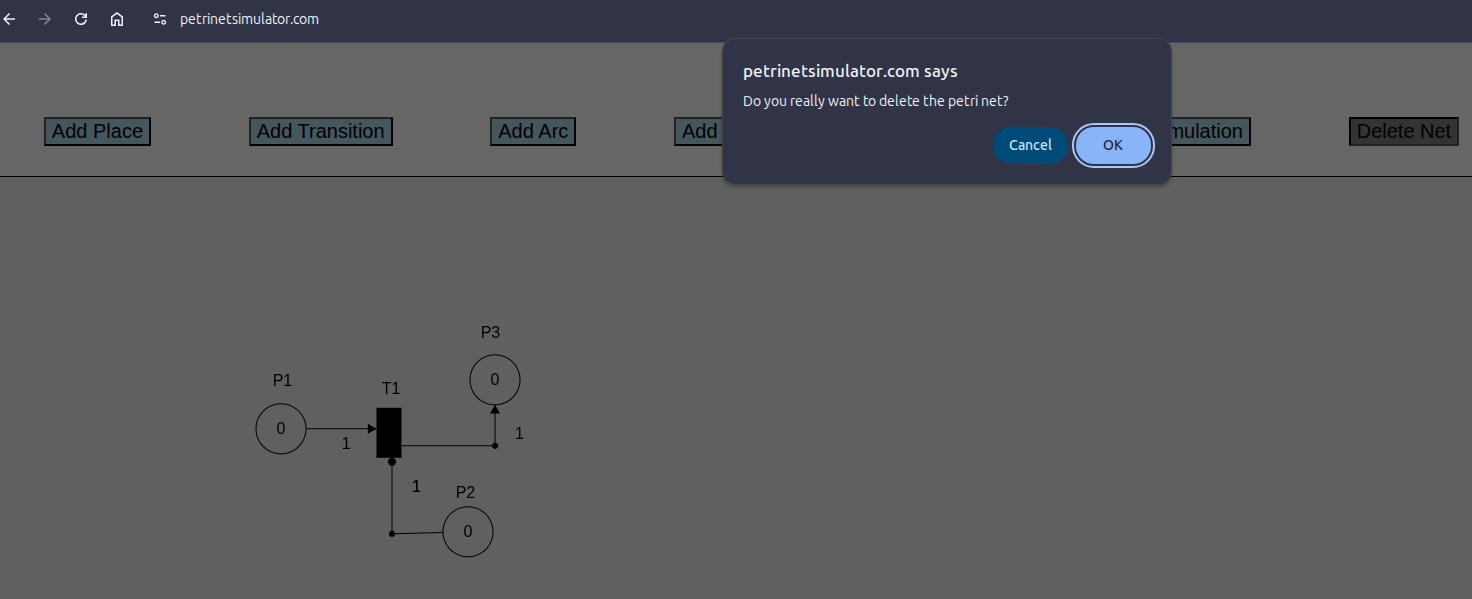
\includegraphics[scale=0.4]{figuras/confirmDeleteNet.png}
	\caption[Caixa de confirmação para exclusão da rede por completo]{Caixa de confirmação para exclusão da rede por completo}
	\label{fig:confirmDeleteNet}
\end{figure}
\FloatBarrier

\lstinputlisting[caption={Código para caixa de confirmação de exclusão da rede por completo}, captionpos=b, label={lst:confirmDeleteNet}]{scripts/confirmDeleteNet.js}

Após a confirmação, por parte do usuário, faz-se a exclusão da rede por completo.

\section{Salvando e carregando a rede}\label{cap:saveLoadNet}

Com a rede de Petri já construída, torna-se essencial disponibilizar mecanismos que permitam seu salvamento e posterior carregamento, garantindo assim a persistência dos dados e a continuidade do trabalho do usuário. Na aplicação web desenvolvida, essas funcionalidades foram implementadas por meio da exportação e importação de arquivos no formato \textbf{JSON}, o que possibilita a portabilidade da rede entre diferentes dispositivos ou sessões. Adicionalmente, a aplicação realiza o salvamento automático no \textbf{\textit{localStorage}} do navegador, permitindo a recuperação da rede de Petri mesmo após o fechamento ou recarregamento da página, evitando perdas acidentais de progresso.

Como citado em capítulos anteriores, a rede de Petri, nada mais é, que a interpretação das várias variáveis ao longo de todo o código \ref{cap:deleteNetFull}. Dessa forma, para que ocorra o salvamento da rede de Petri, é necessário persistir os dados dessas variáveis de maneira simples e portável. Com isso, um arquivo \textbf{\textit{.json}}, contendo todos os dados necessários para a replicação da rede de Petri é exportado sempre que ocorre uma ação de salvamento, através do botão \textbf{\textit{Save Net}} da rede de Petri e, para o carregamento, é feito uma importação, com o botão \textbf{\textit{Load Net}}, desse arquivo \textbf{\textit{.json}}. O formato \textbf{\textit{JSON}} é leve e portável, facilitando o compartilhamento da rede de Petri entre os vários usuários.   

\begin{figure}[ht] 
	\centering
	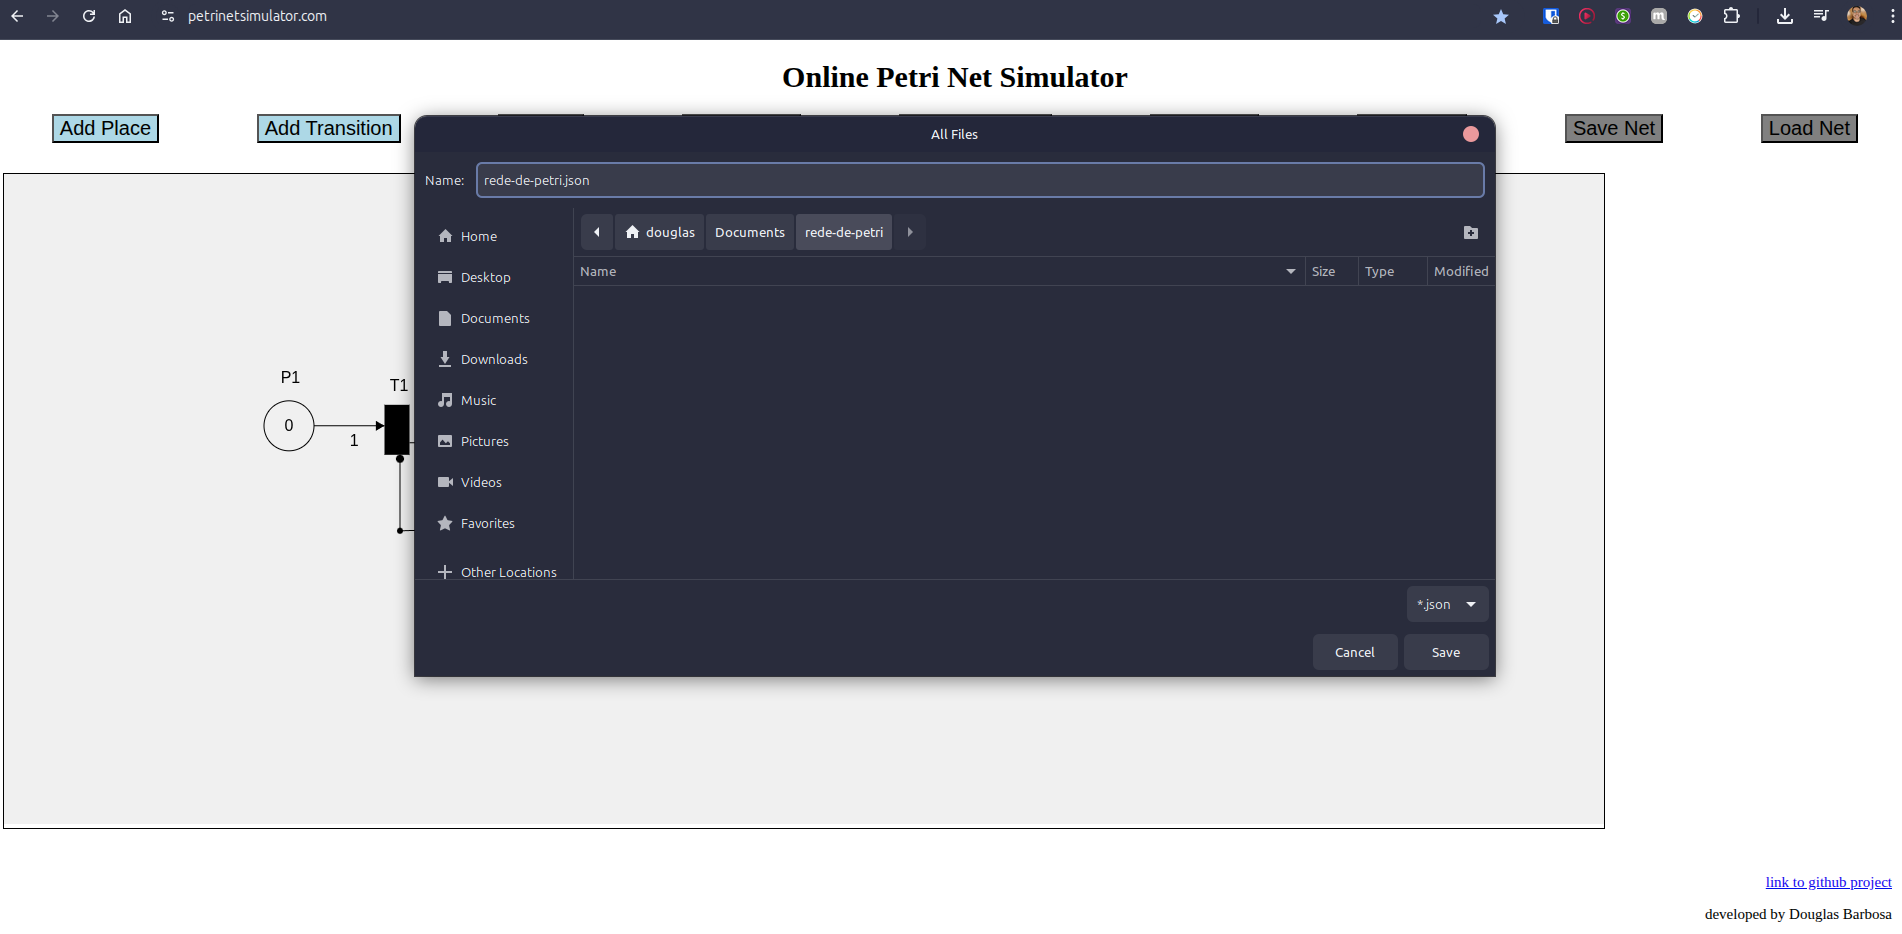
\includegraphics[scale=0.3]{figuras/saveNet.png}
	\caption[Tela para exportação da rede de Petri]{Tela para exportação da rede de Petri}
	\label{fig:saveNet}
\end{figure}
\FloatBarrier

\begin{figure}[ht] 
	\centering
	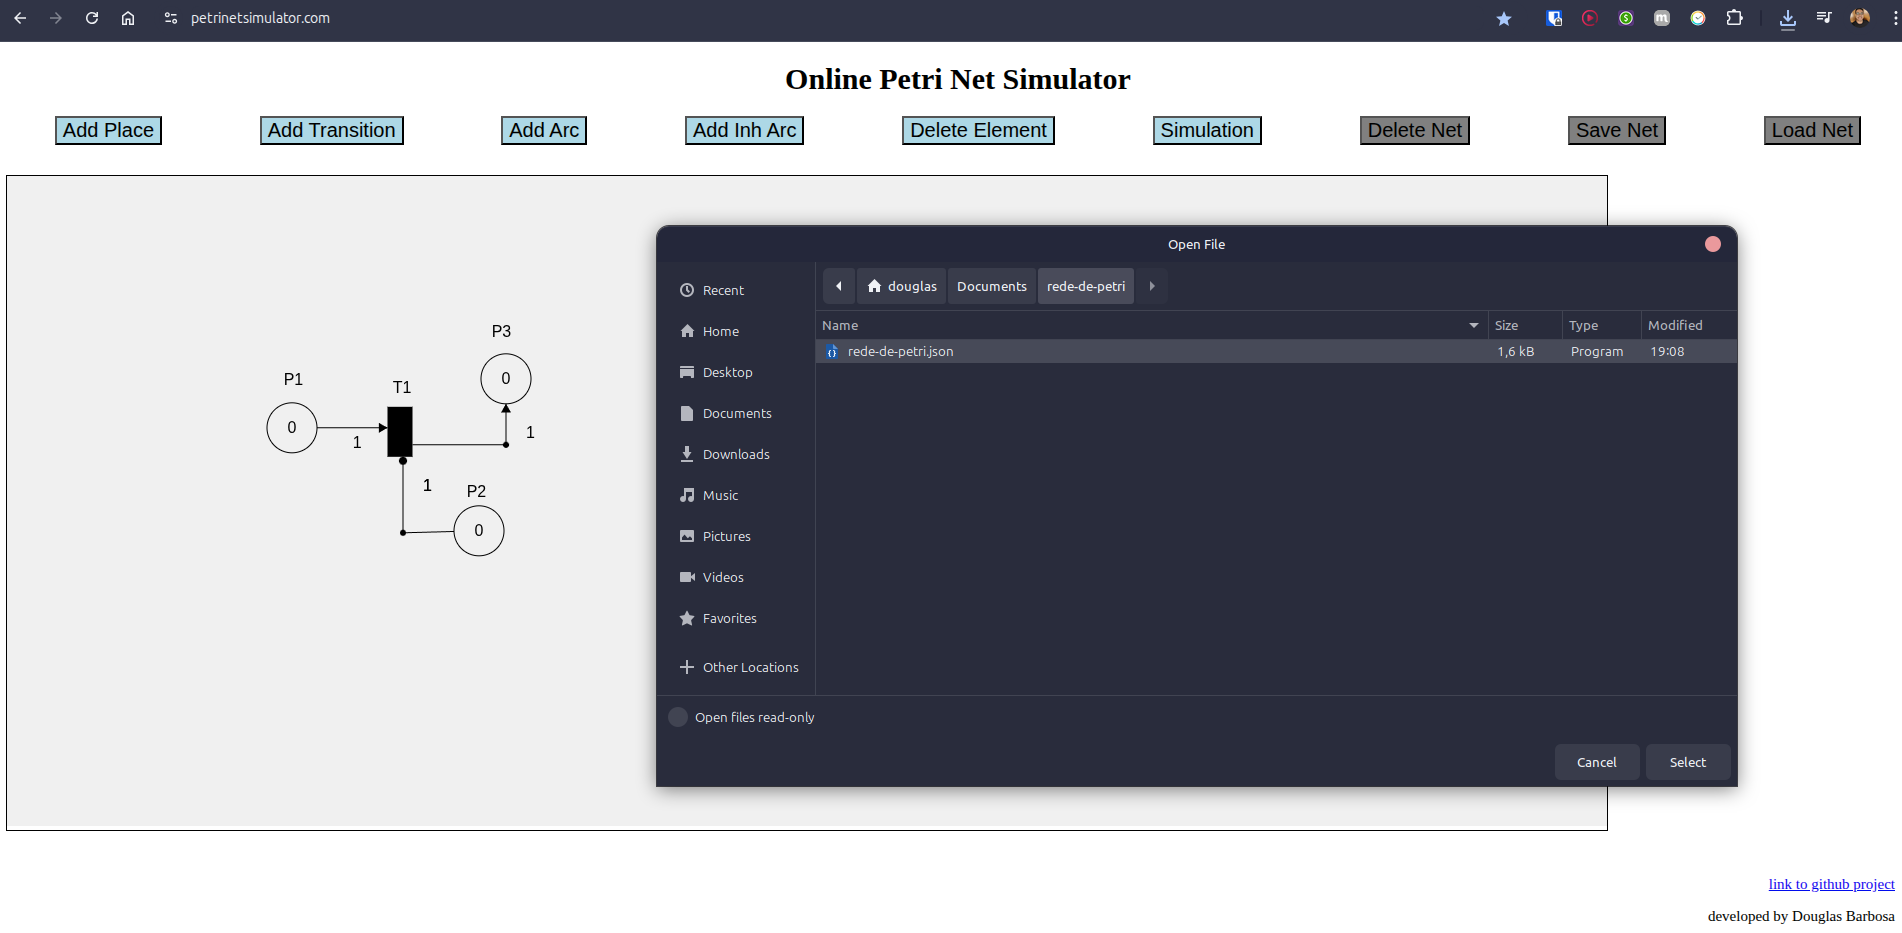
\includegraphics[scale=0.3]{figuras/loadNet.png}
	\caption[Tela para importação da rede de Petri]{Tela para importação da rede de Petri}
	\label{fig:loadNet}
\end{figure}
\FloatBarrier

Para a exportação, após o clique do botão \textbf{\textit{Save Net}}, ocorre a chamada da função \textbf{\textit{saveJSON()}}. Ela chama outra função, \textbf{saveVariables()}, que salva as variáveis. Após, ocorre a exportação dos dados no arquivo \textbf{\textit{.json}} 

\lstinputlisting[caption={Código para exportação da rede num arquivo \textbf{\textit{.json}}}, captionpos=b, label={lst:saveNet}]{scripts/saveNet.js}

Para a importação, após o clique do botão \textbf{\textit{Load Net}}, ocorre a chamada da função \textbf{\textit{loadJSON()}}. Ela chama outra função, \textbf{loadVariables()}, que carrega as variáveis. Após, ocorre a importação dos dados do arquivo \textbf{\textit{.json}} 

\lstinputlisting[caption={Código para importação da rede num arquivo \textbf{\textit{.json}}}, captionpos=b, label={lst:saveNet}]{scripts/loadNet.js}

\subsubsection*{localStorage}\label{cap:localStorage} 

Além da exportação e importação de arquivos \textbf{\textit{.json}}, há também o salvamento através do \textbf{\textit{localStorage}}. O \textbf{\textit{localStorage}} é uma funcionalidade nativa dos navegadores modernos que permite o armazenamento de dados localmente no dispositivo do usuário, de forma persistente e sem necessidade de conexão com o servidor \cite{mdn_local_storage}. 

\lstinputlisting[caption={Código para persistência dos dados com \textbf{\textit{localStorage}}}, captionpos=b, label={lst:localStorage}]{scripts/localStorage.js}

\begin{figure}[ht] 
	\centering
	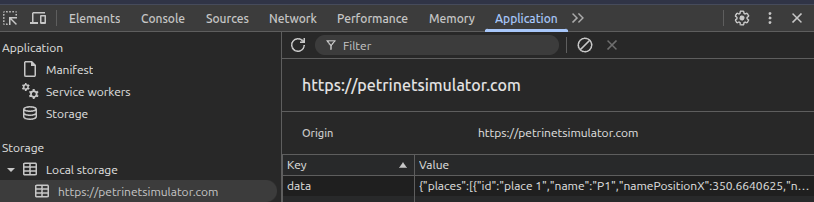
\includegraphics[scale=0.6]{figuras/localStorage.png}
	\caption[Dados persistidos no localStorage]{Dados persistidos no \textbf{\textit{localStorage}}}
	\label{fig:localStorage}
\end{figure}
\FloatBarrier

Na aplicação desenvolvida, o \textbf{\textit{localStorage}} é utilizado como mecanismo complementar de persistência de dados. Sempre que a rede de Petri é modificada, o seu estado atual é convertido para uma representação em formato \textbf{\textit{JSON}} e armazenado localmente. Dessa forma, ao retornar à aplicação, o usuário pode retomar seu trabalho a partir do ponto em que parou, sem a necessidade de realizar uma exportação manual. Esta abordagem contribui significativamente para a usabilidade e robustez da ferramenta, proporcionando uma experiência mais fluida e confiável. 

\section{Simulação da rede} \label{cap:simulation}

A simulação da rede de Petri desenvolvida pelo usuário desempenha um papel fundamental no funcionamento do sistema. Após a criação da rede, torna-se necessário permitir sua manipulação e execução. Como as redes de Petri possuem uma representação matemática bem definida, a simulação pode ser realizada de forma eficiente. Para isso, é necessário comparar, modificar e atualizar as variáveis que compõem a estrutura da rede, como número de marcações dos lugares, peso dos arcos e verificando se uma transição está ativada ou não. 

Para simular a rede de Petri, duas funções principais foram desenvolvidas. A primeira, denominada \textbf{\textit{netSimulationEnables()},} analisa todas as transições, verificando quais delas estão ativadas. Cada transição é analisada individualmente, verificando se as condições para ativação estão sendo cumpridas. Caso sim, a propriedade \textbf{\textit{isEnable}} \ref{prop:isEnable} da transição é definida como \textbf{\textit{true}} e a cor da transição na tela se altera para vermelho \ref{fig:renderTransition}. 

\lstinputlisting[caption={Função \textbf{\textit{netSimulationEnables()}}}, captionpos=b, label={lst:saveNet}]{scripts/transitionEnable.js}

Inicialmente, percorre-se todas as transições analisando quais arcos estão chegando. Essa etapa é feita observando a propriedade \textbf{\textit{connections}} de cada transição. Analisando o peso do arco, em comparação com o número de marcações do lugar em que ele está saindo, determina-se se o arco está ativado ou não.

\begin{description}
	\item[Arcos normais:] número de marcações $\geq$ peso do arco;
	\item[Arcos inibidores:] número de marcações < peso do arco.
\end{description}

Após cada verificação de arco, o resultado é armazenado no \textbf{\textit{arrayIsEnable}}. Caso todas as verificações sejam verdadeiras, a propriedade \textbf{\textit{isEnable}} da transição é alterada para \textbf{\textit{true}}, caso contrário, como \textbf{\textit{false}}. 

A segunda função, denominada \textbf{\textit{netSimulationMove()}}, faz a movimentação das marcações, conforme o usuário clica na transição que está ativada. A função é chamada sempre que ocorre o evento \textbf{\textit{mousedown}} e a variável \textbf{\textit{simulation}} é definida como\textbf{\textit{true}}, o que ocorre sempre que o botão \textbf{\textit{Simulation}} é pressionado.  

\lstinputlisting[caption={Código para ativação da simulação}, captionpos=b, label={lst:enableSimulation}]{scripts/enableSimulation.js}

Tendo a simulação ativada, o usuário deve fazer o clique nas transições que deseja, simulando o comportamento da rede e movimentando as marcações do lugar de origem para o lugar de destino. A função \textbf{\textit{netSimulationMove()}} executa duas ações: 

\begin{enumerate}
	\item subtrair do lugar de origem o número de marcações com base no peso do arco que sai;
	\item adicionar ao lugar de destino o número de marcações com base no peso do arco que chega.
\end{enumerate}

\lstinputlisting[caption={Função \textbf{\textit{netSimulationMove()}}}, captionpos=b, label={lst:netSimulationMove}]{scripts/netSimulationMove.js}

O primeiro passo da função verifica se o clique ocorreu dentro de alguma transição e se ela está ativada. Caso sim, as duas ações ocorrem. A primeira subtrai do lugar de origem o valor correspondente ao peso do arco que está saindo. A segunda soma ao lugar de destino o valor correspondente ao peso de arco. Também, é necessário que os arcos para essas ações sejam do tipo normal. O peso dos arcos inibidores não interferem na subtração ao adição de marcações, apenas na ativação dos arcos.

\begin{figure}[ht] 
	\centering
	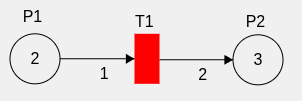
\includegraphics[scale=0.8]{figuras/moveTokens1.png}
	\caption[Movimentando as marcações]{Movimentação das marcações - Parte 1}
	\label{fig:moveTokens1}
\end{figure}
\FloatBarrier

\begin{figure}[ht] 
	\centering
	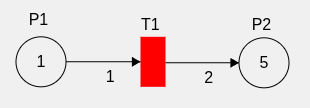
\includegraphics[scale=0.8]{figuras/moveTokens2.png}
	\caption[Movimentando as marcações]{Movimentação das marcações - Parte 2}
	\label{fig:moveTokens2}
\end{figure}
\FloatBarrier

\begin{figure}[ht] 
	\centering
	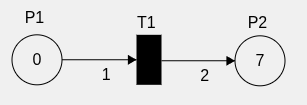
\includegraphics[scale=0.8]{figuras/moveTokens3.png}
	\caption[Movimentando as marcações]{Movimentação das marcações - Parte 3}
	\label{fig:moveTokens3}
\end{figure}
\FloatBarrier

Através da função \textbf{\textit{netSimulationMove()}} simula-se o comportamento da rede de Petri.

\section{Publicação do projeto online}

A publicação do projeto online garante que qualquer usuário com acesso a internet consiga acessar a aplicação web desenvolvida. Com o objetivo de tornar o simulador de redes de Petri acessível, de forma ampla e gratuita, optou-se por realizar sua publicação como uma aplicação web estática, utilizando ferramentas modernas de desenvolvimento e hospedagem. O projeto, desenvolvido integralmente com tecnologias de \textbf{\textit{front-end}}, HTML, CSS e Javascript \ref{cap:tecnologiaweb}, não requer \textbf{\textit{back-end}} ou banco de dados, tornando-o ideal para ser hospedado em plataformas que oferecem suporte a sites estáticos. 

Para o controle de versão e o gerenciamento do código-fonte, utilizou-se a plataforma Github, amplamente reconhecida na área de desenvolvimento de software por oferecer hospedagem de repositórios baseados no sistema de controle de versões Git  \ref{cap:git}. O código-fonte do simulador encontra-se hospedado em um repositório público, o que promove a transparência do desenvolvimento e facilita eventuais colaborações futuras. 

\begin{figure}[ht] 
	\centering
	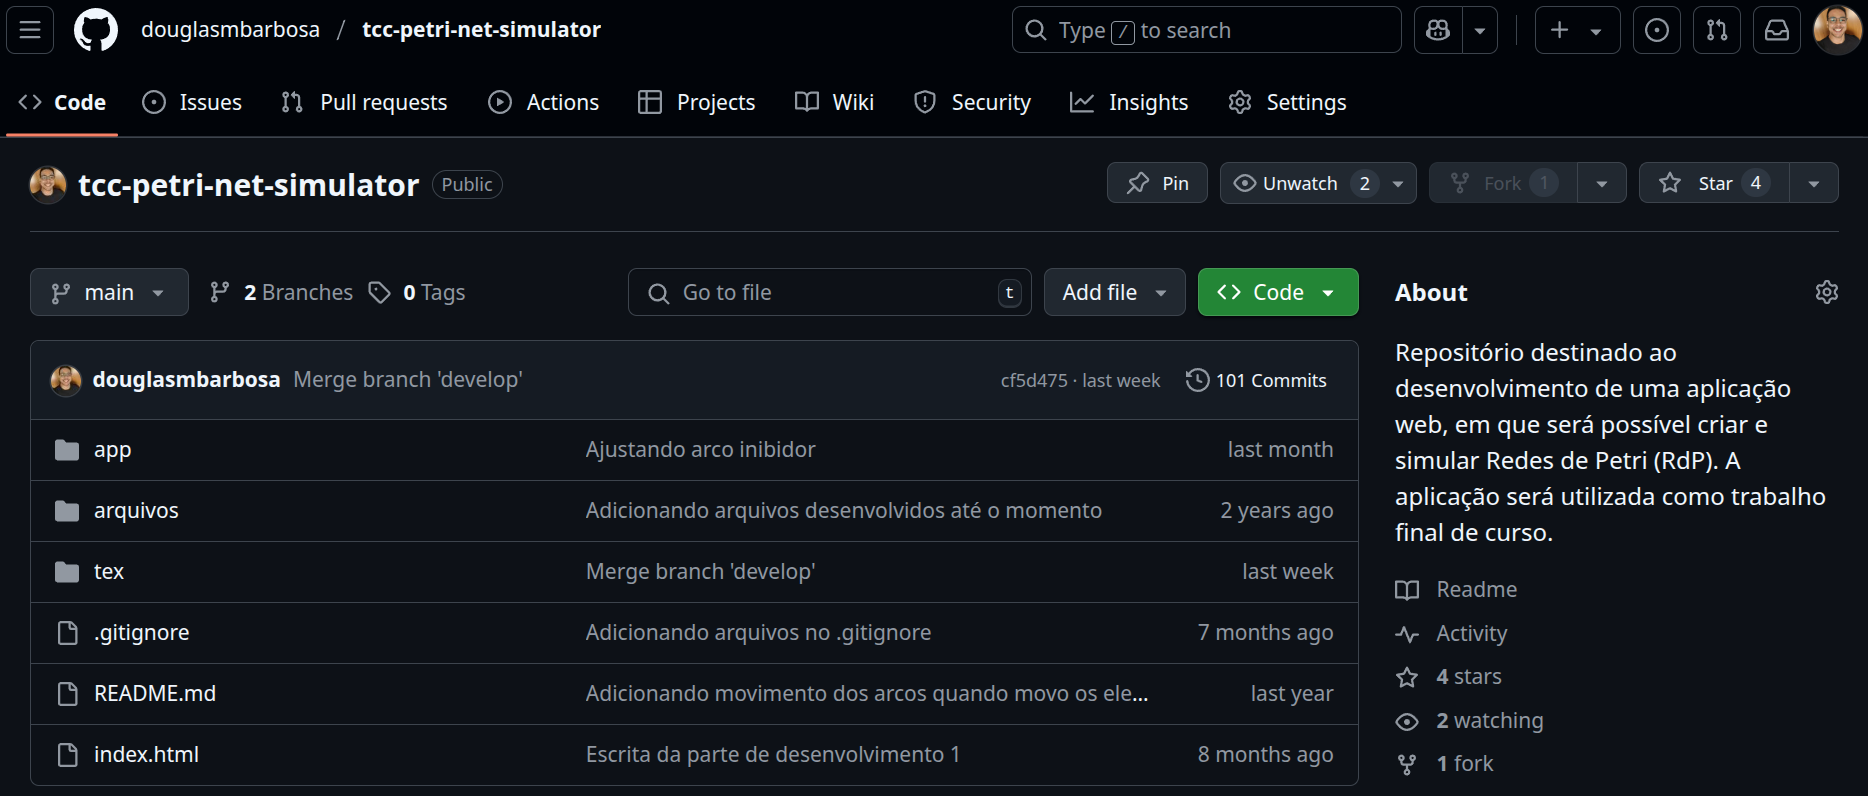
\includegraphics[scale=0.33]{figuras/repoGithub.png}
	\caption[Repositório Github]{Repositório Github:  \href{https://github.com/douglasmbarbosa/tcc-petri-net-simulator}{github.com/douglasmbarbosa/tcc-petri-net-simulator}}
	\label{fig:repoGithub}
\end{figure}
\FloatBarrier

A publicação online e o processo de entrega contínua foram realizados por meio da ferramenta Netlify, uma plataforma de hospedagem focada em aplicações front-end. O Netlify oferece integração nativa com o GitHub, permitindo que cada modificação realizada na \textbf{\textit{branch}} \textbf{\textit{main}} do repositório dispare automaticamente um novo processo de \textbf{\textit{build}} e \textbf{\textit{deploy}} do projeto. Ou seja, sempre que ocorre uma alteração no repositório, faz-se a subida dessas modificações automaticamente para o usuário final. Essa integração contínua garante que a versão publicada do simulador esteja sempre sincronizada com a última versão do código. 

\begin{figure}[ht] 
	\centering
	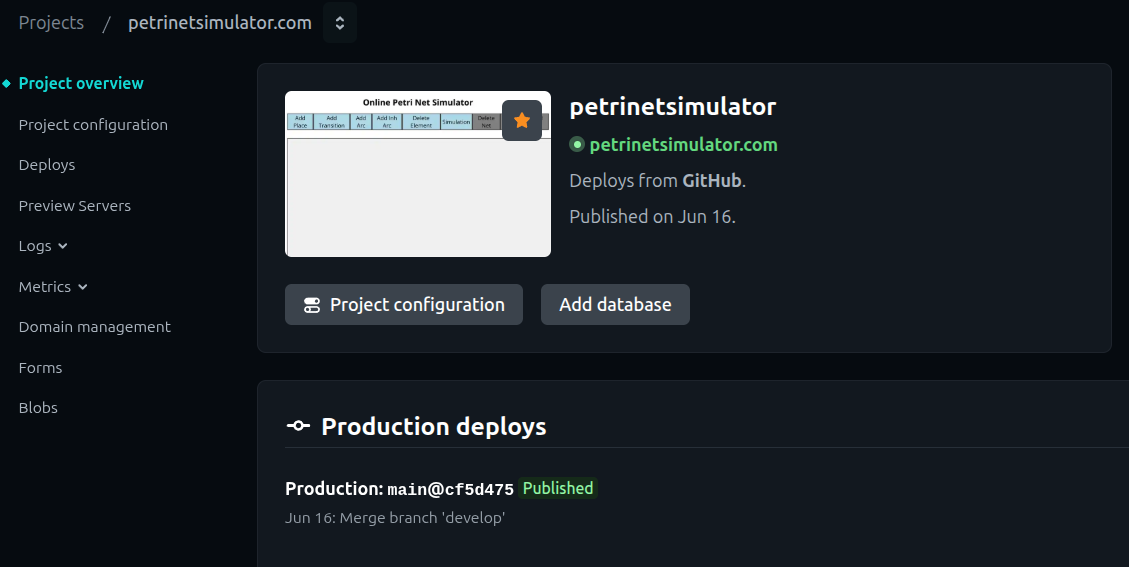
\includegraphics[scale=0.5]{figuras/netlify1.png}
	\caption[netlify 1 ]{Projeto criado na plataforma Netlyfy}
	\label{fig:netlify1}
\end{figure}
\FloatBarrier

Para a configuração do projeto na plataforma Netlify, optou-se pela utilização de um domínio personalizado. O domínio \textbf{\textit{\href{https://petrinetsimulator.com}{petrinetsimulator.com}}} foi adquirido na plataforma Hostinger para a publicação do projeto online. Após a compra do domínio, registrou-se o mesmo na Netlify, juntamente com a integração com o Github. 

\begin{figure}[ht] 
	\centering
	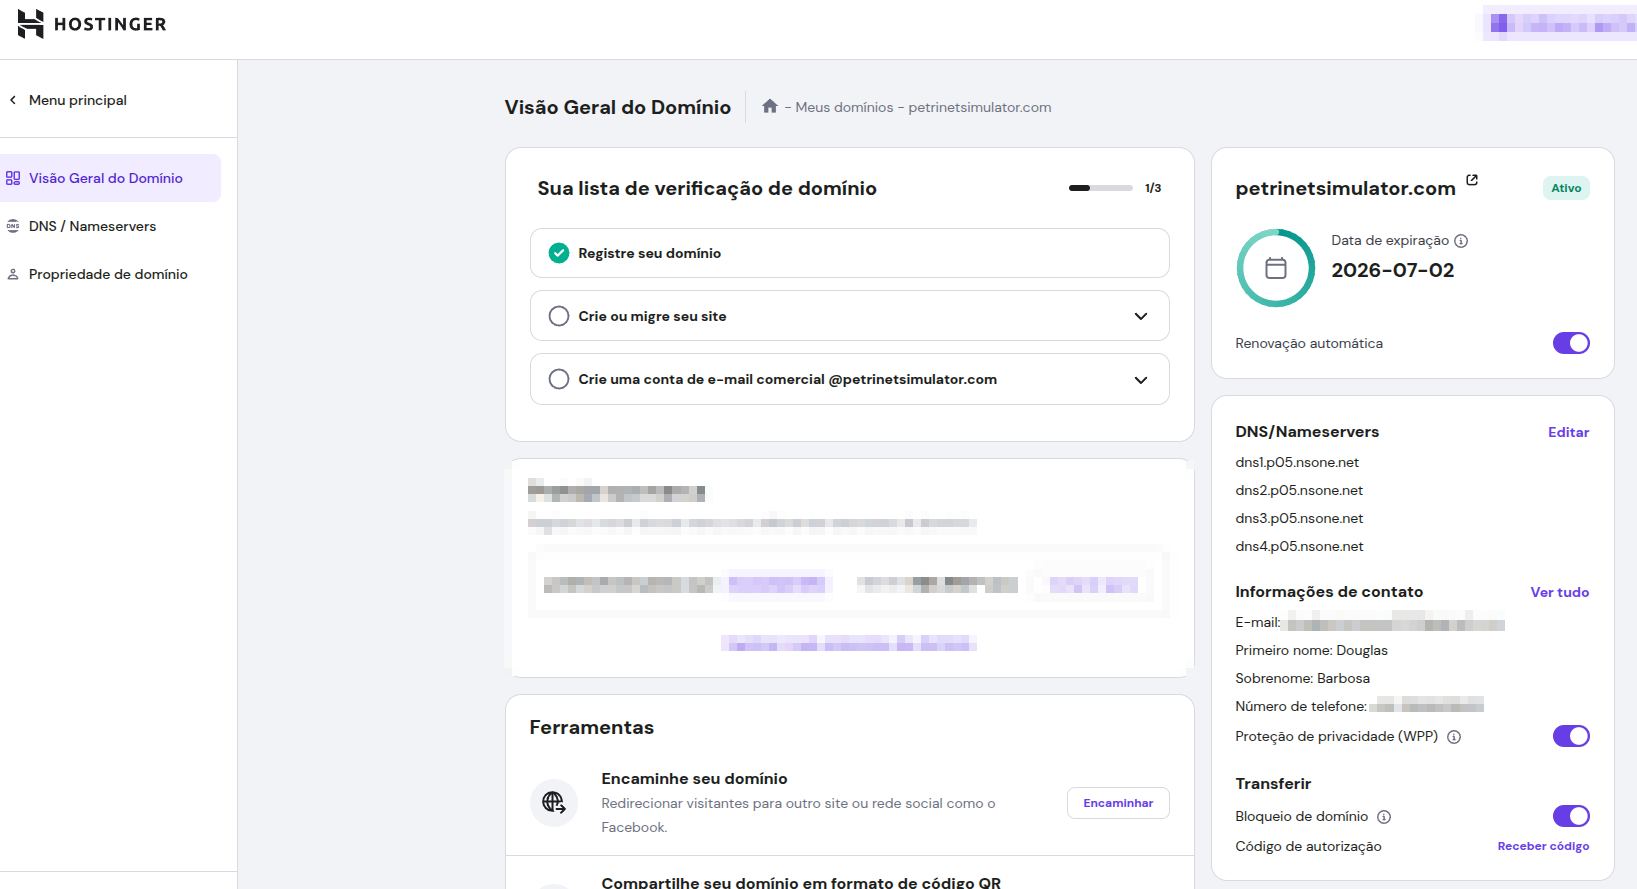
\includegraphics[scale=0.35]{figuras/hostingerDomain.png}
	\caption[Hostinger Domain]{Domínio personalizado na plataforma Hostinger}
	\label{fig:hostinger}
\end{figure}
\FloatBarrier

\begin{figure}[ht] 
	\centering
	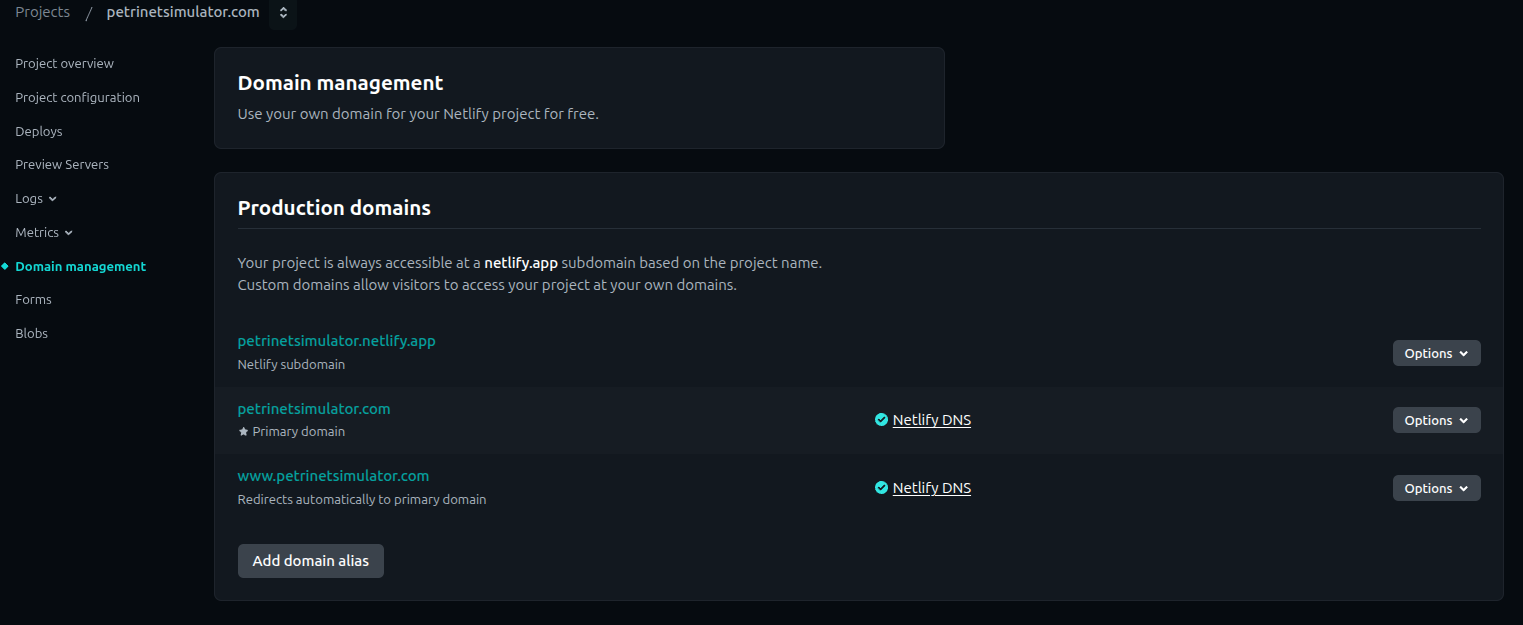
\includegraphics[scale=0.4]{figuras/netlify2.png}
	\caption[netlify 2]{Domínio personalizado configurado na plataforma Netlify}
	\label{fig:netlify2}
\end{figure}
\FloatBarrier

Além dessas configurações, a plataforma Netlify fornece o certificado SSL/TLS, garantindo a utilização do protocolo HTTPS, fornecendo um acesso seguro para os usuário da aplicação web. 

\begin{figure}[ht] 
	\centering
	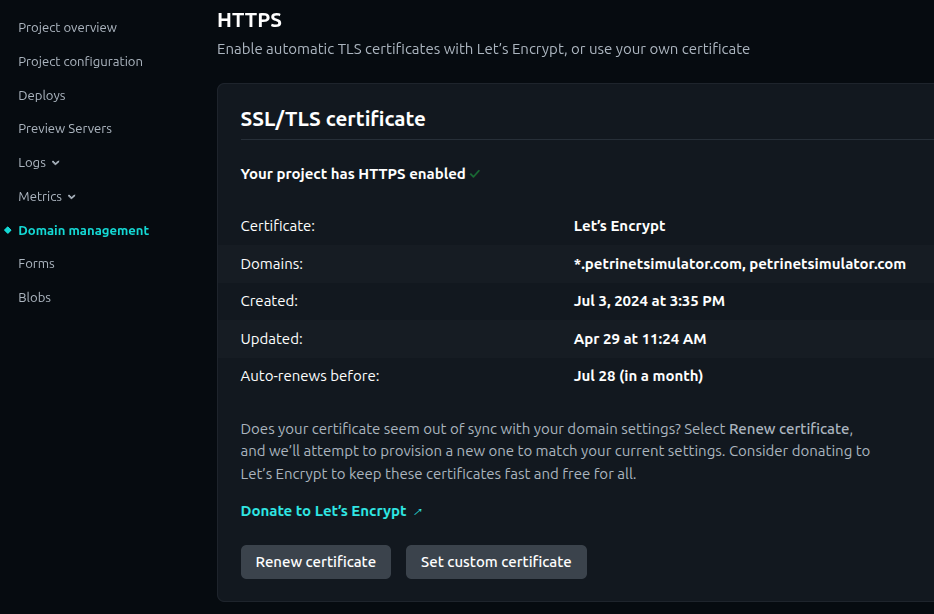
\includegraphics[scale=0.5]{figuras/netlify3.png}
	\caption[netlify 3]{Certificado SSL/TLS configurado na plataforma Netlify}
	\label{fig:netlify2}
\end{figure}
\FloatBarrier

A integração entre as ferramentas adotadas e as práticas empregadas ao longo do desenvolvimento contribuíram para a disponibilização eficiente, segura e acessível, de forma online, ao simulador de redes de Petri. 

% Caso seja um trabalho oriundo da Escola de Minas ou do ICEB, é conveniente apresentar uma fórmula:
% \begin{equation}
% f(x) = \int \limits_{0}^{+ \infty} \tanh \left[\ln (j \omega)^2 \right] dx \,. \label{eq:01}
% \end{equation}

% Lembre-se: equações fazem parte do texto e, por isso, devem ser pontuadas! Assim, conforme a equação \eqref{eq:02}, que está na página \pageref{eq:02}, tem-se uma demonstração. Um outro exemplo é :
% \begin{equation}
% \lim\limits_{x \to 0} \frac{\sin (x)}{x} = 1 \,. 
% \label{eq:02}
% \end{equation}

% Pode-se também escrever equações na linha, como $E = m c^2\,,$ mas somente para expressões menores.

% Se for desenvolvido no ICHS (ver figura \ref{fig:309}), tem-se uma noção melhor do movimento estudantil. A figura \ref{fig:308} ilustra bem o fato.

% % uma figura
% \begin{figure}[h] % o ``h'' significa colocar a figura aqui (here)
% 	\centering
% 	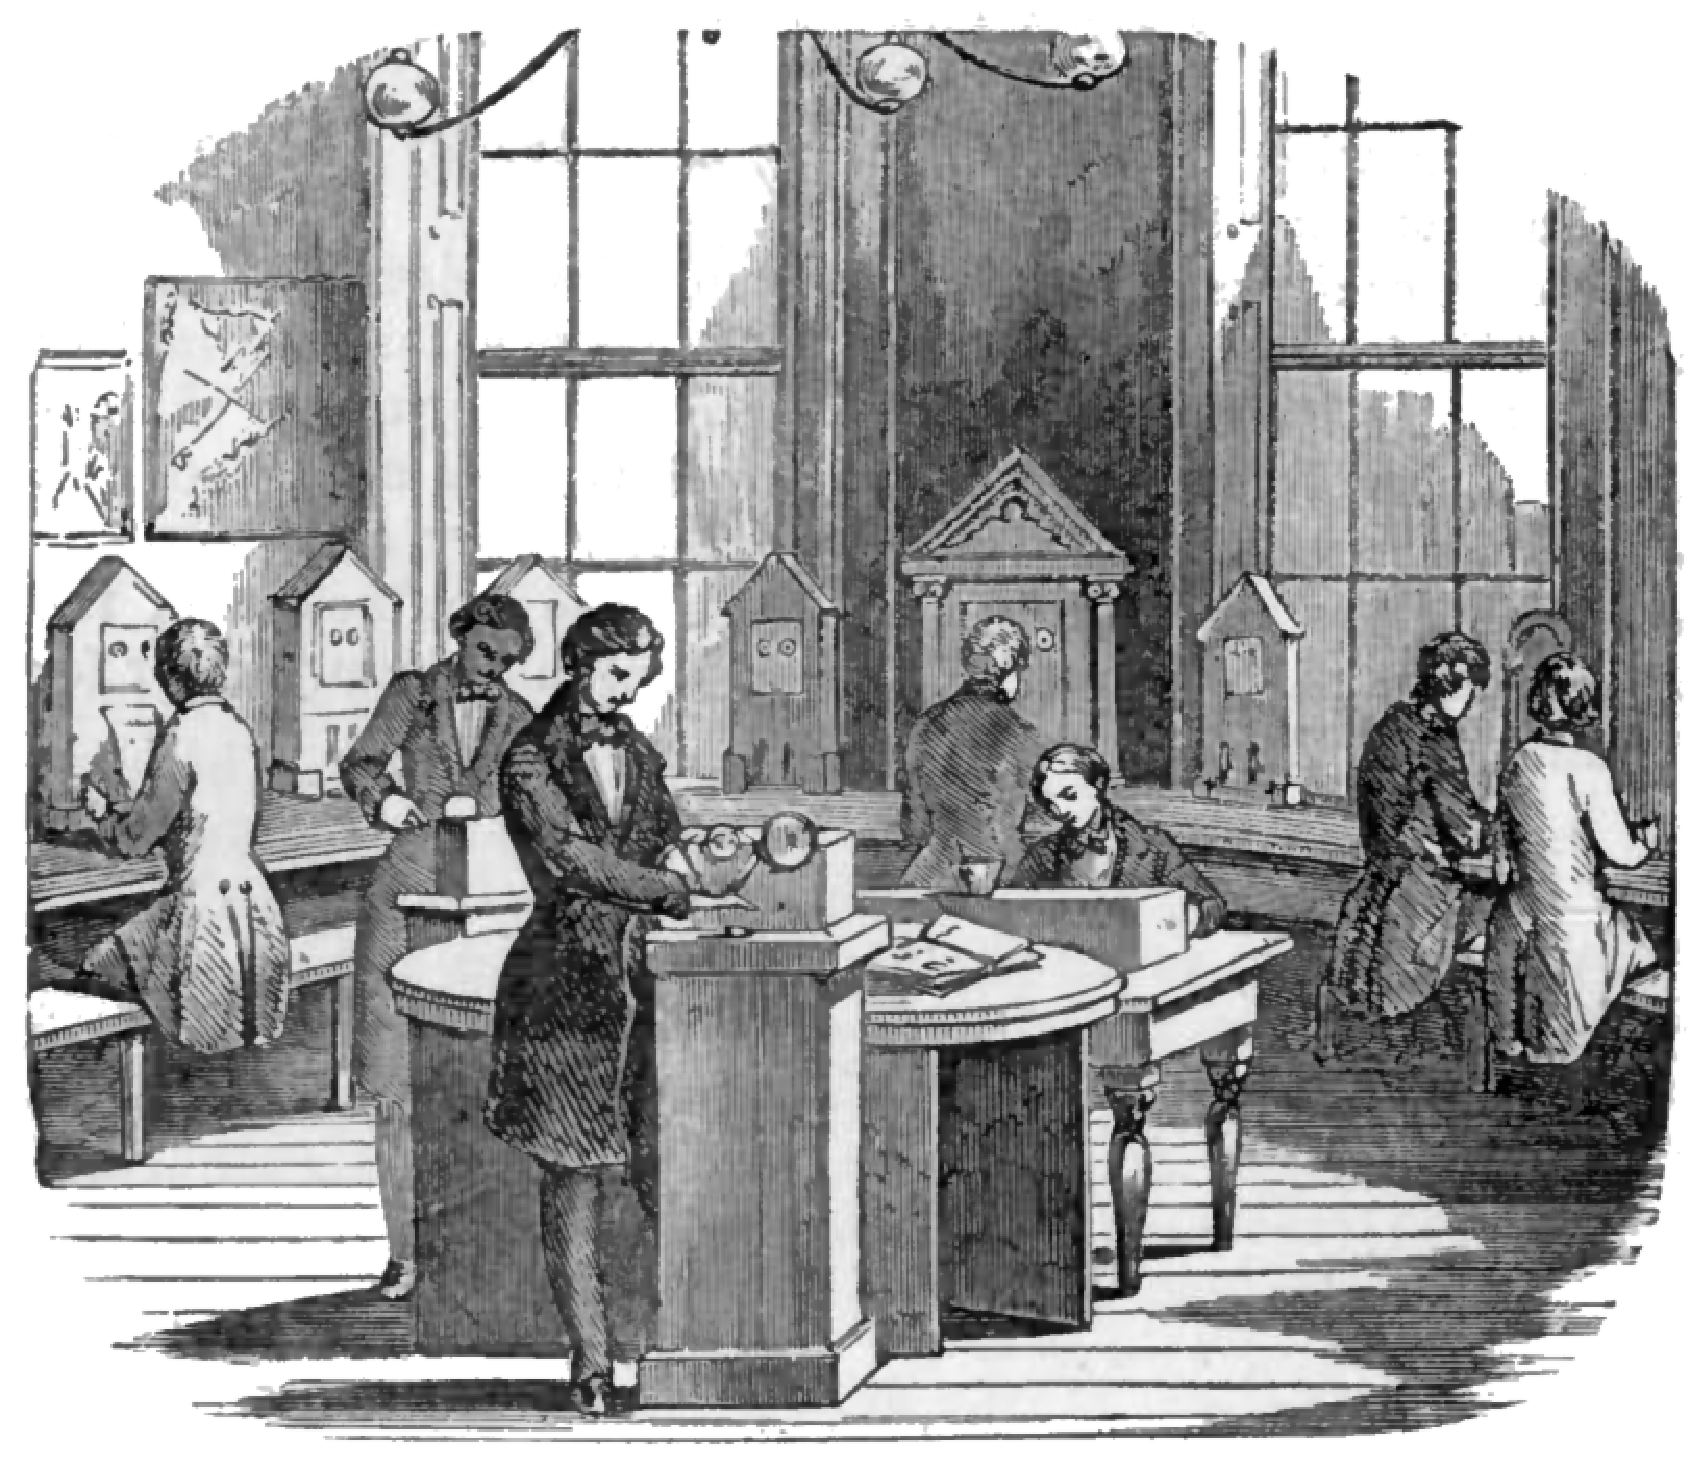
\includegraphics[scale=0.3]{fig09.pdf} % teste os valores
% 	\caption[Legenda reduzida. Aparece apenas no sumário]{Legenda completa - não aparece no sumário. Aqui você pode colocar uma explicação melhor. Fonte: \textcite{boyle1772}.}
% 	\label{fig:308}
% \end{figure}

% \lipsum[22]

% % uma figura
% \begin{figure}[h]
% 	\centering
% 	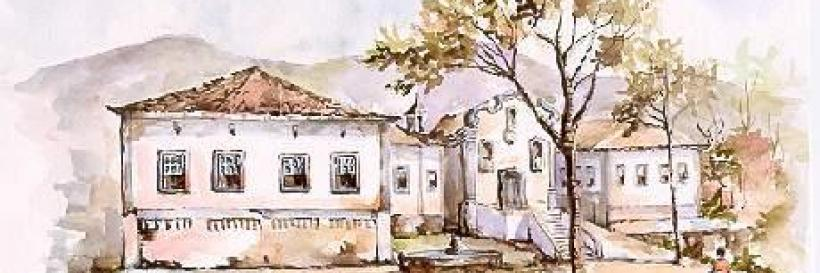
\includegraphics[scale=0.4]{ichs2.jpg} % teste os valores
% 	\caption[Legenda reduzida - aparece apenas no sumário]{Legenda completa - não aparece no sumário. Aqui você pode colocar uma explicação melhor, sem que ela apareça no sumário do seu trabalho. Fonte: \cite[p.~117]{boyle1772}.}
% 	\label{fig:309}
% \end{figure}



% \section{Uma seção extravagante}
% % ---
% \lipsum[21]


% % primeiro capitulo de Resultados
\chapter{Considerações Finais} \label{cap:resultados}

Escrever aqui sobre as expectativas futuras. Pode-se colocar aquilo que ainda pode ser desenvolvido na aplicação, como: redes coloridas, estocásticas, desenvolvimento de uma interface mais agradável, dentre outras melhorias


Falar aqui sobre criação de uma tela de login, e banco de dados para armazenamento das redes de petri criadas. Melhorias de interface como adicionar um texto explicando o que o usuário deve fazer quando executa uma ação.


% % ---

% Neste capítulo é apresentada uma análise dos resultados obtidos.

% \section{Dados, dados, dados}
% % ---
% \lipsum[21]

% % ----------------------------------------------------------
% %\phantompart
% % Insere arquivo de Considerações Finais ou Conclusões
% \chapter{Considerações finais}
% As últimas palavras podem ser apresentadas neste capítulo. Ele pode ser numerado ou não. Caso queria que ele não possua numeração, utilize \* apos o comando chapter.

% \lipsum[21]

% ----------------------------------------------------------
% ELEMENTOS PÓS-TEXTUAIS
% ----------------------------------------------------------
\postextual
% ----------------------------------------------------------

%% ----------------------------------------------------------
%% Referências bibliográficas
%% ----------------------------------------------------------
% toca nome de bibliografia para ``Referências''
\printbibliography%[title=Referências]

% ----------------------------------------------------------
% Glossário
% ----------------------------------------------------------

% Consulte o manual da classe abntex2 para orientações sobre o glossário.

% \glossary

% ----------------------------------------------------------
% Apêndices
% ----------------------------------------------------------
%(Lembre-se: Apendices são de autoria do próprio autor do texto.
% Anexos são elementos de autorias de outros, que o autor do texto julga interessante apresentar)
% ---
% Inicia os apêndices:
% ---
% \begin{apendicesenv}

% % Imprime uma página indicando o início dos apêndices
% %\partapendices
% % ---
% % Insere arquivo com o apêndice A
% % --------

% \chapter{libero justo}
% Lembre-se: apêndices são de autoria do próprio autor do texto. Anexos são elementos de autorias de outros, que o autor do texto julga interessante apresentar


% \end{apendicesenv}
% % ---

% % ----------------------------------------------------------
% % Anexos
% % ----------------------------------------------------------
% %(Lembre-se: Apendices são de autoria do próprio autor do texto.
% % Anexos são elementos de autorias de outros, que o autor do texto julga interessante apresentar)
% % ---
% % Inicia os anexos
% % ---
% \begin{anexosenv}

% % Imprime uma página indicando o início dos anexos
% %\partanexos

% % ---
% % Insere arquivo com os anexos 1, 2
% \chapter{Morbi ultrices rutrum lorem.}
% Lembre-se: apêndices são de autoria do próprio autor do texto. Anexos são elementos de autorias de outros, que o autor do texto julga interessante apresentar

% \chapter{Lorem Morbi ultrices rutrum.}
% Lembre-se: apêndices são de autoria do próprio autor do texto. Anexos são elementos de autorias de outros, que o autor do texto julga interessante apresentar

% % ---
% \end{anexosenv}

% %---------------------------------------------------------------------
% % INDICE REMISSIVO
% %---------------------------------------------------------------------
% %\phantompart
% \printindex
% %---------------------------------------------------------------------

\end{document}